\PassOptionsToPackage{unicode=true}{hyperref} % options for packages loaded elsewhere
\PassOptionsToPackage{hyphens}{url}
\PassOptionsToPackage{dvipsnames,svgnames*,x11names*}{xcolor}
%
\documentclass[12pt,]{krantz}
\usepackage{lmodern}
\usepackage{amssymb,amsmath}
\usepackage{ifxetex,ifluatex}
\usepackage{fixltx2e} % provides \textsubscript
\ifnum 0\ifxetex 1\fi\ifluatex 1\fi=0 % if pdftex
  \usepackage[T1]{fontenc}
  \usepackage[utf8]{inputenc}
  \usepackage{textcomp} % provides euro and other symbols
\else % if luatex or xelatex
  \usepackage{unicode-math}
  \defaultfontfeatures{Ligatures=TeX,Scale=MatchLowercase}
\fi
% use upquote if available, for straight quotes in verbatim environments
\IfFileExists{upquote.sty}{\usepackage{upquote}}{}
% use microtype if available
\IfFileExists{microtype.sty}{%
\usepackage[]{microtype}
\UseMicrotypeSet[protrusion]{basicmath} % disable protrusion for tt fonts
}{}
\IfFileExists{parskip.sty}{%
\usepackage{parskip}
}{% else
\setlength{\parindent}{0pt}
\setlength{\parskip}{6pt plus 2pt minus 1pt}
}
\usepackage{xcolor}
\usepackage{hyperref}
\hypersetup{
            pdftitle={Machine Learning Básico},
            pdfauthor={Synergy Vision},
            colorlinks=true,
            linkcolor=Maroon,
            filecolor=Maroon,
            citecolor=Blue,
            urlcolor=Blue,
            breaklinks=true}
\urlstyle{same}  % don't use monospace font for urls
\usepackage{color}
\usepackage{fancyvrb}
\newcommand{\VerbBar}{|}
\newcommand{\VERB}{\Verb[commandchars=\\\{\}]}
\DefineVerbatimEnvironment{Highlighting}{Verbatim}{commandchars=\\\{\}}
% Add ',fontsize=\small' for more characters per line
\usepackage{framed}
\definecolor{shadecolor}{RGB}{248,248,248}
\newenvironment{Shaded}{\begin{snugshade}}{\end{snugshade}}
\newcommand{\AlertTok}[1]{\textcolor[rgb]{0.94,0.16,0.16}{#1}}
\newcommand{\AnnotationTok}[1]{\textcolor[rgb]{0.56,0.35,0.01}{\textbf{\textit{#1}}}}
\newcommand{\AttributeTok}[1]{\textcolor[rgb]{0.77,0.63,0.00}{#1}}
\newcommand{\BaseNTok}[1]{\textcolor[rgb]{0.00,0.00,0.81}{#1}}
\newcommand{\BuiltInTok}[1]{#1}
\newcommand{\CharTok}[1]{\textcolor[rgb]{0.31,0.60,0.02}{#1}}
\newcommand{\CommentTok}[1]{\textcolor[rgb]{0.56,0.35,0.01}{\textit{#1}}}
\newcommand{\CommentVarTok}[1]{\textcolor[rgb]{0.56,0.35,0.01}{\textbf{\textit{#1}}}}
\newcommand{\ConstantTok}[1]{\textcolor[rgb]{0.00,0.00,0.00}{#1}}
\newcommand{\ControlFlowTok}[1]{\textcolor[rgb]{0.13,0.29,0.53}{\textbf{#1}}}
\newcommand{\DataTypeTok}[1]{\textcolor[rgb]{0.13,0.29,0.53}{#1}}
\newcommand{\DecValTok}[1]{\textcolor[rgb]{0.00,0.00,0.81}{#1}}
\newcommand{\DocumentationTok}[1]{\textcolor[rgb]{0.56,0.35,0.01}{\textbf{\textit{#1}}}}
\newcommand{\ErrorTok}[1]{\textcolor[rgb]{0.64,0.00,0.00}{\textbf{#1}}}
\newcommand{\ExtensionTok}[1]{#1}
\newcommand{\FloatTok}[1]{\textcolor[rgb]{0.00,0.00,0.81}{#1}}
\newcommand{\FunctionTok}[1]{\textcolor[rgb]{0.00,0.00,0.00}{#1}}
\newcommand{\ImportTok}[1]{#1}
\newcommand{\InformationTok}[1]{\textcolor[rgb]{0.56,0.35,0.01}{\textbf{\textit{#1}}}}
\newcommand{\KeywordTok}[1]{\textcolor[rgb]{0.13,0.29,0.53}{\textbf{#1}}}
\newcommand{\NormalTok}[1]{#1}
\newcommand{\OperatorTok}[1]{\textcolor[rgb]{0.81,0.36,0.00}{\textbf{#1}}}
\newcommand{\OtherTok}[1]{\textcolor[rgb]{0.56,0.35,0.01}{#1}}
\newcommand{\PreprocessorTok}[1]{\textcolor[rgb]{0.56,0.35,0.01}{\textit{#1}}}
\newcommand{\RegionMarkerTok}[1]{#1}
\newcommand{\SpecialCharTok}[1]{\textcolor[rgb]{0.00,0.00,0.00}{#1}}
\newcommand{\SpecialStringTok}[1]{\textcolor[rgb]{0.31,0.60,0.02}{#1}}
\newcommand{\StringTok}[1]{\textcolor[rgb]{0.31,0.60,0.02}{#1}}
\newcommand{\VariableTok}[1]{\textcolor[rgb]{0.00,0.00,0.00}{#1}}
\newcommand{\VerbatimStringTok}[1]{\textcolor[rgb]{0.31,0.60,0.02}{#1}}
\newcommand{\WarningTok}[1]{\textcolor[rgb]{0.56,0.35,0.01}{\textbf{\textit{#1}}}}
\usepackage{longtable,booktabs}
% Fix footnotes in tables (requires footnote package)
\IfFileExists{footnote.sty}{\usepackage{footnote}\makesavenoteenv{longtable}}{}
\usepackage{graphicx,grffile}
\makeatletter
\def\maxwidth{\ifdim\Gin@nat@width>\linewidth\linewidth\else\Gin@nat@width\fi}
\def\maxheight{\ifdim\Gin@nat@height>\textheight\textheight\else\Gin@nat@height\fi}
\makeatother
% Scale images if necessary, so that they will not overflow the page
% margins by default, and it is still possible to overwrite the defaults
% using explicit options in \includegraphics[width, height, ...]{}
\setkeys{Gin}{width=\maxwidth,height=\maxheight,keepaspectratio}
\setlength{\emergencystretch}{3em}  % prevent overfull lines
\providecommand{\tightlist}{%
  \setlength{\itemsep}{0pt}\setlength{\parskip}{0pt}}
\setcounter{secnumdepth}{5}
% Redefines (sub)paragraphs to behave more like sections
\ifx\paragraph\undefined\else
\let\oldparagraph\paragraph
\renewcommand{\paragraph}[1]{\oldparagraph{#1}\mbox{}}
\fi
\ifx\subparagraph\undefined\else
\let\oldsubparagraph\subparagraph
\renewcommand{\subparagraph}[1]{\oldsubparagraph{#1}\mbox{}}
\fi

% set default figure placement to htbp
\makeatletter
\def\fps@figure{htbp}
\makeatother

\usepackage[T1]{fontenc}
\usepackage[utf8]{inputenc} % recommended encoding
\usepackage[spanish]{babel}
\usepackage{booktabs}
\usepackage{longtable}
\usepackage[bf,singlelinecheck=off]{caption}

%\setmainfont[UprightFeatures={SmallCapsFont=AlegreyaSC-Regular}]{Alegreya}

\usepackage{framed,color}
\definecolor{shadecolor}{RGB}{248,248,248}

\renewcommand{\textfraction}{0.05}
\renewcommand{\topfraction}{0.8}
\renewcommand{\bottomfraction}{0.8}
\renewcommand{\floatpagefraction}{0.75}

\renewenvironment{quote}{\begin{VF}}{\end{VF}}
\let\oldhref\href
\renewcommand{\href}[2]{#2\footnote{\url{#1}}}

\ifxetex
  \usepackage{letltxmacro}
  \setlength{\XeTeXLinkMargin}{1pt}
  \LetLtxMacro\SavedIncludeGraphics\includegraphics
  \def\includegraphics#1#{% #1 catches optional stuff (star/opt. arg.)
    \IncludeGraphicsAux{#1}%
  }%
  \newcommand*{\IncludeGraphicsAux}[2]{%
    \XeTeXLinkBox{%
      \SavedIncludeGraphics#1{#2}%
    }%
  }%
\fi

\makeatletter
\newenvironment{kframe}{%
\medskip{}
\setlength{\fboxsep}{.8em}
 \def\at@end@of@kframe{}%
 \ifinner\ifhmode%
  \def\at@end@of@kframe{\end{minipage}}%
  \begin{minipage}{\columnwidth}%
 \fi\fi%
 \def\FrameCommand##1{\hskip\@totalleftmargin \hskip-\fboxsep
 \colorbox{shadecolor}{##1}\hskip-\fboxsep
     % There is no \\@totalrightmargin, so:
     \hskip-\linewidth \hskip-\@totalleftmargin \hskip\columnwidth}%
 \MakeFramed {\advance\hsize-\width
   \@totalleftmargin\z@ \linewidth\hsize
   \@setminipage}}%
 {\par\unskip\endMakeFramed%
 \at@end@of@kframe}
\makeatother

\renewenvironment{Shaded}{\begin{kframe}}{\end{kframe}}

\newenvironment{rmdblock}[1]
  {
  \begin{itemize}
  \renewcommand{\labelitemi}{
    \raisebox{-.7\height}[0pt][0pt]{
      {\setkeys{Gin}{width=3em,keepaspectratio}\includegraphics{images/#1}}
    }
  }
  \setlength{\fboxsep}{1em}
  \begin{kframe}
  \item
  }
  {
  \end{kframe}
  \end{itemize}
  }
\newenvironment{rmdnote}
  {\begin{rmdblock}{note}}
  {\end{rmdblock}}
\newenvironment{rmdcaution}
  {\begin{rmdblock}{caution}}
  {\end{rmdblock}}
\newenvironment{rmdimportant}
  {\begin{rmdblock}{important}}
  {\end{rmdblock}}
\newenvironment{rmdtip}
  {\begin{rmdblock}{tip}}
  {\end{rmdblock}}
\newenvironment{rmdwarning}
  {\begin{rmdblock}{warning}}
  {\end{rmdblock}}

\usepackage{makeidx}
\makeindex

\urlstyle{tt}

\usepackage{amsthm}
\makeatletter
\def\thm@space@setup{%
  \thm@preskip=8pt plus 2pt minus 4pt
  \thm@postskip=\thm@preskip
}
\makeatother

\frontmatter
\usepackage[]{natbib}
\bibliographystyle{apalike}

\title{Machine Learning Básico}
\providecommand{\subtitle}[1]{}
\subtitle{Ciencia de los Datos Financieros}
\author{Synergy Vision}
\date{2019-06-26}

\let\BeginKnitrBlock\begin \let\EndKnitrBlock\end
\begin{document}
\maketitle

%\cleardoublepage\newpage\thispagestyle{empty}\null
%\cleardoublepage\newpage\thispagestyle{empty}\null
%\cleardoublepage\newpage
\thispagestyle{empty}

\setlength{\abovedisplayskip}{-5pt}
\setlength{\abovedisplayshortskip}{-5pt}

{
\hypersetup{linkcolor=}
\setcounter{tocdepth}{2}
\tableofcontents
}
\listoftables
\listoffigures
\hypertarget{prefacio}{%
\chapter*{Prefacio}\label{prefacio}}



\includegraphics{images/by-nc-sa.png}\\
La versión en línea de este libro se comparte bajo la licencia \href{http://creativecommons.org/licenses/by-nc-sa/4.0/}{Creative Commons Attribution-NonCommercial-ShareAlike 4.0 International License}.

\hypertarget{por-que-leer-este-libro}{%
\section*{¿Por qué leer este libro?}\label{por-que-leer-este-libro}}


Este libro aspira a que las empresas iberoamericanas tengan un acceso fácil y en su propio idioma a una tecnología que les permitirá el manejo estratégico de sus datos para soportar mejor la toma de decisiones sobre sus negocios. Para ello, el libro aportará con ejemplos muy diversos del mundo empresarial, las herramientas básicas del Machine Learning, haciendo énfasis en las aplicaciones prácticas con ayuda de los softwares R y Phyton, sin requerir mayores complicaciones matemáticas o computacionales. Los lenguajes de programación Python y R, son sin duda, los más utilizados a la hora de construir modelos de inteligencia artificial.

El material expuesto en el libro se concentra en precisar las técnicas más comunes usadas en Machine Learning, para que las empresas o individuos interesados, tengan un punto de partida sólido sobre el cual ir construyendo un conjunto de herramientas que puedan utilizar en cualquier momento. El lector podrá aprender las principales librerías y dominar la sintaxis para la construcción de modelos.

Contar con este conocimiento es una gran ventaja, pues el gran avance de internet en la última década ha hecho crecer de forma exponencial la cantidad de datos que se producen por la interacción con sus usuarios. Así, poder crear modelos que permitan sacar ventaja a partir de estos datos, se ha vuelto una meta imprescindible para la mayoría de las empresas en el mundo actual, dado que en dichos datos se encuentran patrones que siguen clientes y usuarios. Los individuos o empresas que logren develar estos patrones, tendrán una enorme ventaja estratégica sobre sus competidores en el mundo actual. Esperamos que este libro pueda ayudarlos en esa tarea.

\hypertarget{estructura-del-libro}{%
\section*{Estructura del libro}\label{estructura-del-libro}}


Este libro se divide en 7 capítulos, en los cuales se especificarán las instrucciones técnicas para poder acceder a los programas y funciones a utilizar. Cada sección estará compuesta por una sección teórica, seguida de la sintaxis requerida para la construcción de los modelos. En la mayoría de los casos está información es proporcionada a través de imágenes donde el lector observará cómo aplicar la sintaxis de forma adecuada.

La secuencia de ejemplos de uso de las herramientas siempre se presentará primero en R y luego en Phyton.\\
El propósito de este material es ofrecer una experiencia de aprendizaje distinta y enfocada en el estudiante de forma que realmente aprenda y practique con mucha intensidad. La idea es cambiar el modelo de clases magistrales y ofrecer una experiencia más centrada en el estudiante y menos centrado en el profesor. Para los temas más técnicos y avanzados es necesario trabajar de la mano con el estudiante y asistirlo en el proceso de aprendizaje con prácticas guiadas, material en línea e interactivo, videos, evaluación continua de brechas y entendimiento, entre otros, para procurar el dominio de la materia.

\hypertarget{informacion-sobre-los-programas-y-convenciones}{%
\section*{Información sobre los programas y convenciones}\label{informacion-sobre-los-programas-y-convenciones}}


A lo largo de este material estaremos usando las palabras \emph{paquetes y librerías}
, las cuales se refieren a lo mismo, la única diferencia es la preferencia de uso entre las comunidades que utilizan los diversos lenguajes de programación. De igual forma, usaremos la palabra función o método, las cuales si bien presentan algunas diferencias entre ellas dependiendo del lenguaje utilizado, tienen en general para este curso, el mismo significado. Por tal razón las usaremos indistintamente, dado que las variaciones solo son relevantes mencionarlas en un curso avanzado de programación.

Las definiciones en el libro irán en \textbf{negrita}, mientras que los nombres de paquetes y funciones se escribirán en \emph{cursivas}.

\hypertarget{acerca-del-autor}{%
\section*{Acerca del Autor}\label{acerca-del-autor}}


Synergy Vision es una empresa que se especializa en proveer la Formación, la Tecnología y la Consultoría en las áreas de Especulación (Trading), Inversión, Economía, Finanzas y Riesgo.

Ofrecemos Formación de Alto Nivel para prácticas de Consultoría y Ejercicio Profesional Especializado para alcanzar Certificaciones reconocidas a nivel mundial como el CFA, CMT y FRM.

Aplicamos técnicas que conjugan lo que hoy en día se conoce como Data Science que consiste en la aplicación de herramientas de las Matemáticas, Estadísticas y las Ciencias de la Computación, además de las técnicas de Minería de Datos (Datamining) y Aprendizaje de máquina (Machine Learning).

Nuestra oferta de servicios consiste en asistir a empresas con sus canales Electrónicos con aplicaciones Web y Móvil para ofrecer servicios del mundo de la Especulación, Inversiones, Economía, Finanzas y Riesgo. Así como el desarrollo de sistemas especializados para facilitar la gestión de inversiones, portafolios, trading, simuladores, modelos, plataformas de trading, finanzas corporativas, finanzas internacionales, valoración, optimización, riesgo, calculadoras, proyecciones, etc.

Iniciamos la conformación de un ecosistema para materializar esta oferta. En este sentido estamos buscando aliados que en medio de entornos complejos son capaces de identificar oportunidades y materializarlas.

Synergy Vision se encuentra desarrollando y actualizando nuevos materiales sobre temas como: Probabilidad y Estadística Matemática en R, Programación Científica en R, Mercados, Inversiones y Trading, Datos y Modelos Financieros en R, Renta Fija, Inmunización de Carteras de Renta Fija, Teoría de Riesgo en R, Finanzas Cuantitativas, Ingeniería Financiera, Procesos Estocásticos en R, Series de Tiempo en R, Ciencia de los Datos, Ciencia de los Datos Financieros, Simulación en R, Desarrollo de Aplicaciones Interactivas en R, Minería de Datos, Aprendizaje Estadístico, Estadística Multivariante, Riesgo de Crédito, Riesgo de Liquidez, Riesgo de Mercado, Riesgo Operacional, Riesgo de Cambio, Análisis Técnico, Inversión Visual, Finanzas, Finanzas Corporativas, Valoración, Teoría de Portafolio, entre otros.

Nuestra página web: \url{http://synergy.vision/nosotros/}
Nuestra cuenta de Twitter es (\url{https://twitter.com/bysynergyvision}) y nuestros repositorios están en GitHub (\url{https://github.com/synergyvision}).
Somos Científicos de Datos.

\hypertarget{agradecimientos}{%
\section*{Agradecimientos}\label{agradecimientos}}


Este libro es posible gracias a una gran cantidad de desarrolladores que contribuyen en la construcción de herramientas para generar documentos enriquecidos e interactivos. En particular al autor de los paquetes Yihui Xie xie(2015).

A todo el equipo de Synergy Vision que no deja de soñar. Hay que hacer lo que pocos hacen, insistir, insistir hasta alcanzar. Lo más importante es concretar las ideas. La idea es sólo el inicio y solo vale cuando se concreta.

\BeginKnitrBlock{flushright}
Synergy Vision, Caracas, Venezuela
\EndKnitrBlock{flushright}

\mainmatter

\hypertarget{introduccion}{%
\chapter{Introducción}\label{introduccion}}

A diferencia del pasado cuando la información masiva era un lujo permitido solo a las grandes corporaciones públicas o privadas, hoy día gracias a la ubicuidad de las tecnologías digitales, casi cualquier persona o pequeño negocio puede, con poco esfuerzo, recibir ingentes cantidades de datos, sea a través del acceso a bases de datos, internet, comercio en línea, telefonía celular, redes sociales, sensores, transacciones comerciales, registros financieros, mensajería de texto, voz, audio y video, entre muchas otras. Además, los datos fluyen en una policromía de formatos análogos y digitales, como texto en papel o digital, imágenes, fotografías, archivos de audio y video, bases de datos, streaming, entre otras. A esta enorme cantidad de datos se le conoce como Big Data, y ahora tenemos el problema contrario, es decir cómo salir adelante en nuestros emprendimientos sin perdernos entre tanta información. Sin embargo es posible extraer pistas útiles de allí mediante un proceso conocido como minería de datos o data mining en inglés, y la tecnología clave para esta tarea es el machine learning o aprendizaje automático.

El machine learning es parte de la Ciencia de Datos o Data Science y fue creado para estudiar teorías, algoritmos y aplicaciones de sistemas que aprenden como los humanos. Su empleo es cada vez más amplio debido a que proporciona estrategias probadas para descubrir patrones entre miles o millones de datos. La extensión de su uso se debe a dos factores: el primero es la ya comentada accesibilidad a grandes volúmenes de información y el segundo, es la aparición de herramientas computacionales para manejarlos a costos cada vez más reducidos y con tecnologías asequibles, mediante softwares de código abierto como R y Python.

Los softwares de código abierto son publicados bajo una licencia de código abierto o forman parte del dominio público. En el caso de R y Phyton pueden descargarse libremente y existe una comunidad de usuarios y desarrolladores que de manera gratuita y colaboradora, los mantienen actualizados y en constante mejora, con nuevas y cada vez más poderosas aplicaciones. De manera que el único obstáculo real para el uso del machine learning por parte del público de habla española de España y América Latina es su desconocimiento.
Aparte de estudios académicos formales universitarios, existen excelentes recursos a los cuales acceder para el dominio del machine Learning. Sin embargo, la inmensa mayoría de estos últimos se encuentran en inglés o en otros idiomas. Además, suelen utilizar un lenguaje cargado de tecnicismos computacionales, matemáticos o estadísticos, que alejan a la mayoría, más interesada en resolver los urgentes problemas de su negocio o profesión, que en sumergirse en los oscuros detalles de un teorema. Por esta razón ofrecemos este texto en español a los empresarios, emprendedores, profesionales y estudiantes de pregrado y de postgrado de cualquier disciplina de España y América Latina, en una presentación que esperamos resulte especialmente útil, por su orientación práctica y libre de complicaciones excesivamente técnicas.
En este libro se presentan ejemplos y algoritmos de varias técnicas de machine learning, que pueden ser comprendidos por cualquiera con un dominio matemático y estadístico básico, al nivel del primer o segundo año de la mayoría de las disciplinas del pregrado universitario, en España y América Latina. Por ello, esperamos que un público muy vasto pueda beneficiarse del contenido de este libro.

\hypertarget{clasificacion-de-los-aprendizajes}{%
\section{Clasificación de los Aprendizajes}\label{clasificacion-de-los-aprendizajes}}

Este libro se desarrolla siguiendo la visión estándar de dividir al machine learning en grandes clases o tipologías según el tipo de datos disponibles: \textbf{supervised learning} o \textbf{aprendizaje supervisado}, \textbf{unsupervised learning} o \textbf{aprendizaje no supervisado}, y \textbf{reinforcement learning} o \textbf{aprendizaje reforzado} o por \textbf{refuerzo}.
El aprendizaje supervisado sería el tipo más fundamental de machine learning, en el cual una computadora aprende de un usuario a través de preguntas y respuestas. La computadora aprende a vincular una pregunta con su respuesta a partir de muestras apareadas de preguntas y respuestas. El objetivo es que la computadora adquiera la capacidad de generalización, generando una respuesta apropiada a preguntas no aprendidas. De este modo, el usuario no tiene que enseñarle todo a la computadora, sino que ella puede hacer frente automáticamente a situaciones desconocidas aprendiendo sólo una fracción de conocimiento. El aprendizaje supervisado se ha aplicado con éxito a una amplia gama de temas, como el reconocimiento de escritura a mano, habla e imágenes, filtrado de spam, publicidad online, análisis de señales neuronales, análisis genético, predicción del precio de acciones, pronóstico del tiempo, entre muchos más. El aprendizaje supervisado es conocido como \textbf{regresión} si la respuesta es un valor real como la temperatura; \textbf{clasificación} o problema de reconocimiento de patrones, si la respuesta es un valor categórico como ``sí'' o ``no''. Entre estos destacan los llamados \textbf{árboles de decisión} y los \textbf{random forest} o \textbf{bosques aleatorios}. Finalmente tenemos el \textbf{ranking} u \textbf{ordinal regression}, conocido en español como \textbf{ordenación}, si la respuesta es un valor ordinal como ``bueno'', ``normal'' o ``pobre''.

El aprendizaje no supervisado considera la situación donde no existe un usuario que actúe como orientador de la computadora, la cual recopila datos de forma autónoma a través de Internet u otra fuente de datos, e intenta extraer conocimientos útiles. El aprendizaje no supervisado es más automático que el aprendizaje supervisado, y su objetivo no necesariamente se especifica de manera clara. Entre las tareas típicas del aprendizaje no supervisado está la agrupación de datos y la detección de valores atípicos. Estas técnicas se utilizan con éxito en una amplia gama de problemas como el diagnóstico de sistemas, seguridad, detección de eventos y análisis de redes sociales. También se utiliza a menudo como un paso de preprocesamiento del aprendizaje supervisado. Entre las técnicas más conocidas se encuentran: \textbf{detección de outliers} y de \textbf{novedades}; \textbf{análisis de componentes principales} más conocido por sus siglas en inglés \textbf{PCA} de \textbf{Principal Components Analysis}; \textbf{clustering}; y \textbf{bosques aleatorios}. El \textbf{clustering} o \textbf{agrupamiento} es una parte no supervisada de la clasificación, y su objetivo es categorizar las muestras de entrada en clústeres o grupos sin ninguna supervisión. Por lo general, se supone que muestras similares pertenecen al mismo grupo, y se supone que las muestras disímiles pertenecen a grupos diferentes. Por lo tanto, cómo medir la similitud entre las muestras es la cuestión clave en la agrupación. La detección de outliers o valores atípicos, tiene por objeto encontrar muestras irregulares en un conjunto de datos determinado. El objetivo de la detección de cambios o de novedad, es juzgar si un nuevo conjunto de datos tiene la misma propiedad que el conjunto de datos original.

El aprendizaje por refuerzo está orientado a adquirir la capacidad de generalización de la misma manera que en el aprendizaje supervisado, sin embargo el usuario que actúa como supervisor no responde directamente a las preguntas sino que evalúa el comportamiento del sistema y le proporciona retroalimentación al respecto. El objetivo del aprendizaje por refuerzo es que en base a la retroalimentación del supervisor, le permita a la computadora mejorar su comportamiento para maximizar el resultado de la evaluación. El aprendizaje por refuerzo es un modelo importante para el comportamiento de los humanos y los robots, y se ha aplicado a varias áreas, tales como el control autónomo de robots, juegos de computadora y estrategias de optimización de mercadeo. Detrás del aprendizaje por refuerzo, se utilizan a menudo los métodos de aprendizajes supervisados y no supervisados tales como como regresión, clasificación y agrupamiento. En este libro no abordaremos esta metodología.

\hypertarget{organizacion-del-texto}{%
\section{Organización del texto}\label{organizacion-del-texto}}

El libro se estructura en ocho capítulos, el \textbf{Capítulo 1} corresponde a la presente Introducción, mientras que en el \textbf{Capítulo 2} se inicia al lector en el uso de los softwares R y Phyton, mostrando como proceder a realizar su instalación dentro del ambiente de Anaconda. En todos los capítulos siguientes se sigue el mismo orden de presentación del \textbf{Capítulo 2}, mostrando primero el uso del software R y luego el uso de Python para cada técnica estudiada.

El \textbf{Capítulo 3} se dedica a la lectura y preparación de los datos. En este capítulo introducimos al lector en la técnica de detección de valores atípicos, las cuales pueden ser objeto de aprendizajes supervisados, no supervisados o una combinación de los anteriores.

El \textbf{Capítulo 4} se dedica a la regresión lineal, inicio básico para todos los métodos de regresión. En el \textbf{Capítulo 5} analizamos la regresión logística, esencial en problemas con datos cualitativos o categóricos. Ambas técnicas de regresión corresponden a aprendizajes supervisados. En en el \textbf{Capítulo 6} veremos una de las técnicas más usadas de aprendizaje no supervisado como es el análisis de clúster. Continuamos en el \textbf{Capítulo 7} con este tipo de aprendizaje, introduciendo las bases del análisis de componentes principales (PCA), utilizado como preprocesamiento para otras técnicas como la regresión lineal, porque permite reducir la dimensionalidad de las variables. En el \textbf{Capítulo 8}, investigamos métodos básicos basados en árboles de decisión incluyendo bosques aleatorios.
Como parte integrante del texto se anexan los códigos en R y Python de cada práctica, los cuales pueden descargarse en XXXXXX

En el \textbf{Apéndice} se incluyen información adicional sobre los softwares utilizados y otros relacionados, mientras que las \textbf{Referencias} se presentan otras fuentes para aquellos interesados en continuar profundizando en el tema, aunque se tiene previsto la elaboración de otros recursos para avanzar en el conocimiento de la Ciencia de Datos.

\hypertarget{conjunto-de-bases-de-datos-utilizadas}{%
\section{Conjunto de Bases de Datos utilizadas}\label{conjunto-de-bases-de-datos-utilizadas}}

Algunas de las bases de datos utilizadas fueron creadas directamente para emplearlas en el libro. Otras pueden recuperarse fácilmente con ayuda de los códigos de R y Phyton, dado que son parte de las librerías de estos softwares o vienen por defecto con los mismos. La Tabla 1 a continuación contiene una breve descripción de las mismas:

Tabla 1. Descripción de las bases de datos utilizadas en el libro

\begin{longtable}[]{@{}ccc@{}}
\toprule
\begin{minipage}[b]{0.07\columnwidth}\centering
Nombre\strut
\end{minipage} & \begin{minipage}[b]{0.32\columnwidth}\centering
Librería o ubicación\strut
\end{minipage} & \begin{minipage}[b]{0.52\columnwidth}\centering
Descripción\strut
\end{minipage}\tabularnewline
\midrule
\endhead
\begin{minipage}[t]{0.07\columnwidth}\centering
Default\strut
\end{minipage} & \begin{minipage}[t]{0.32\columnwidth}\centering
ISLR\strut
\end{minipage} & \begin{minipage}[t]{0.52\columnwidth}\centering
Registros de clientes con incumplimiento de pagos de una empresa de tarjetas de crédito\strut
\end{minipage}\tabularnewline
\begin{minipage}[t]{0.07\columnwidth}\centering
Employee Salaries\strut
\end{minipage} & \begin{minipage}[t]{0.32\columnwidth}\centering
\url{https://data.montgomerycountymd.gov/api/views/2qd6-mr43/rows.csv?accessType=DOWNLOAD}\strut
\end{minipage} & \begin{minipage}[t]{0.52\columnwidth}\centering
Salarios de empleados del Condado Montgomery\strut
\end{minipage}\tabularnewline
\begin{minipage}[t]{0.07\columnwidth}\centering
Iris- IrisP\strut
\end{minipage} & \begin{minipage}[t]{0.32\columnwidth}\centering
Distribución básica de R\strut
\end{minipage} & \begin{minipage}[t]{0.52\columnwidth}\centering
Variedades morfológicas de la flor Iris de tres especies relacionadas\strut
\end{minipage}\tabularnewline
\begin{minipage}[t]{0.07\columnwidth}\centering
mtcars\strut
\end{minipage} & \begin{minipage}[t]{0.32\columnwidth}\centering
Distribución básica de R\strut
\end{minipage} & \begin{minipage}[t]{0.52\columnwidth}\centering
Consumo de combustible, caballos de fuerza y otra información sobre 32 automóviles.,Son datos extraídos de la revista Motor Trend US de 1974\strut
\end{minipage}\tabularnewline
\begin{minipage}[t]{0.07\columnwidth}\centering
slsummar\strut
\end{minipage} & \begin{minipage}[t]{0.32\columnwidth}\centering
\url{http://www.fns.usda.gov/sites/default/files/pd/slsummar.xls}\strut
\end{minipage} & \begin{minipage}[t]{0.52\columnwidth}\centering
Participación y almuerzos servidos de 1969 a 2018 por el Programa Nacional de Almuerzo Escolar de EEUU\strut
\end{minipage}\tabularnewline
\begin{minipage}[t]{0.07\columnwidth}\centering
USArrest\strut
\end{minipage} & \begin{minipage}[t]{0.32\columnwidth}\centering
Distribución básica de R\strut
\end{minipage} & \begin{minipage}[t]{0.52\columnwidth}\centering
Estadísticas de delitos por cada 100.000 residentes en 50 estados de EE.UU.\strut
\end{minipage}\tabularnewline
\bottomrule
\end{longtable}

\hypertarget{ambientes-de-trabajo-para-el-cientifico-de-datos}{%
\chapter{Ambientes de trabajo para el científico de datos}\label{ambientes-de-trabajo-para-el-cientifico-de-datos}}

Para usar las herramientas estadísticas y matemáticas, los científicos de datos usan lenguajes de programación que nos ahorran el trabajo de codificar paso a paso los algoritmos de los métodos a utilizar. La comunidad científica nos proporcionan estas soluciones a través de paquetes y librerías que podemos acceder generalmente de manera gratuita. El siguiente gráfico del portal web \url{https://www.paradigmadigital.com/dev/es-python-el-lenguaje-del-futuro/} muestra los lenguajes preferidos por los científicos de datos :

\begin{figure}
\centering
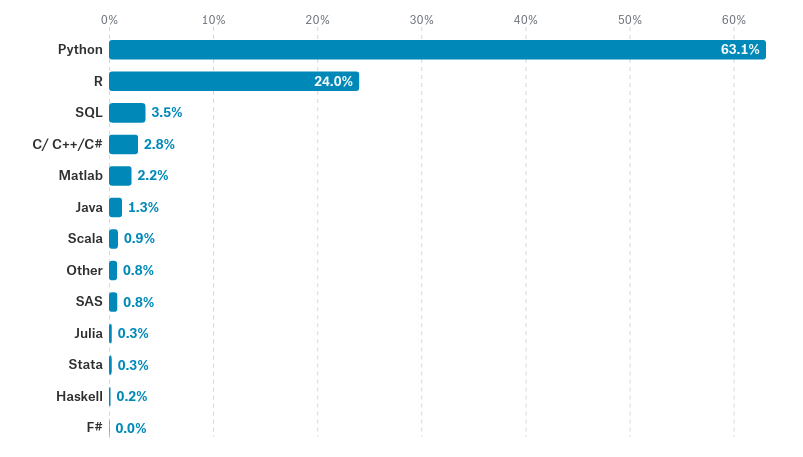
\includegraphics{images/languages.png}
\caption{\label{fig:"sd"}}
\end{figure}

Sin duda \emph{Python} y \emph{R} son los favoritos. Ambos son de códigos abiertos (open source), Phyton es un lenguaje flexible fácil de aprender y de propósito general, adaptable a fines empresariales. Por su parte, R es un lenguaje funcional orientado a la comunidad científica que trabaja con estadísticas, disponiendo de una infinidad de librerías, siempre en crecimiento. Entre ambos lenguajes Phyton es el más utilizado, sin embargo R puede adaptarse para fines empresariales gracias a librerías como Shiny, las cuales permiten crear páginas web donde se pueden aplicar prácticamente todas las herramientas de R y ofrecer resultados adecuados a todo tipo de usuarios.

En principio todo aquel que trabaje con datos debe conocer ambos lenguajes y utilizarlos de acuerdo a sus necesidades. En los ámbitos académicos, divulgativos o de investigación, es recomendable usar R. Phyton es una mejor opción si las necesidades son del campo empresarial, industrial o para el diseño de software en el cual se usen métodos estadísticos. Los dos lenguajes pueden descargarse en los siguientes enlaces:

\begin{itemize}
\item
  \emph{R}: \url{https://www.r-project.org}
\item
  \emph{Python}: \url{https://www.python.org}
\end{itemize}

\hypertarget{primer-encuentro-con-los-lenguajes}{%
\section{Primer encuentro con los lenguajes}\label{primer-encuentro-con-los-lenguajes}}

Al descagar estos lenguajes lo primero que veremos es: en el caso de \emph{R}:

\begin{figure}
\centering
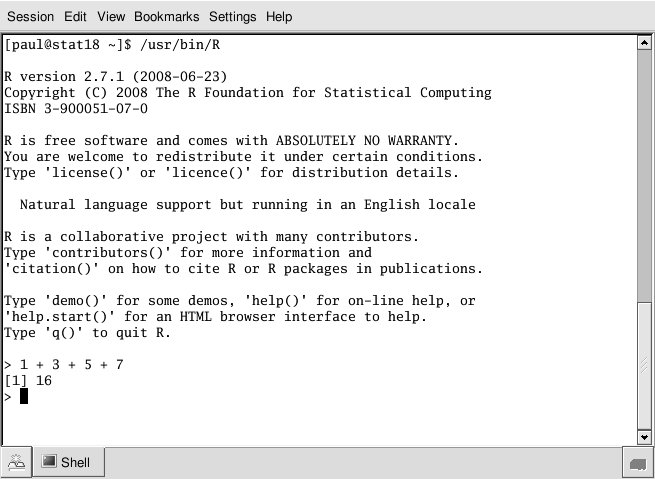
\includegraphics{images/R.png}
\caption{\label{fig:"R"}}
\end{figure}

y en el caso de \emph{Python}:
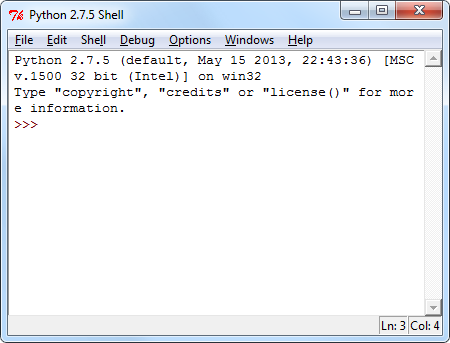
\includegraphics{images/python.png}

Aunque es posible comenzar a trabajar en estos ambientes, lo usual es elegir entornos más amigables.

Para R, el entorno más utilizado es RStudio el cual tiene la siguiente presentación:

\begin{figure}
\centering
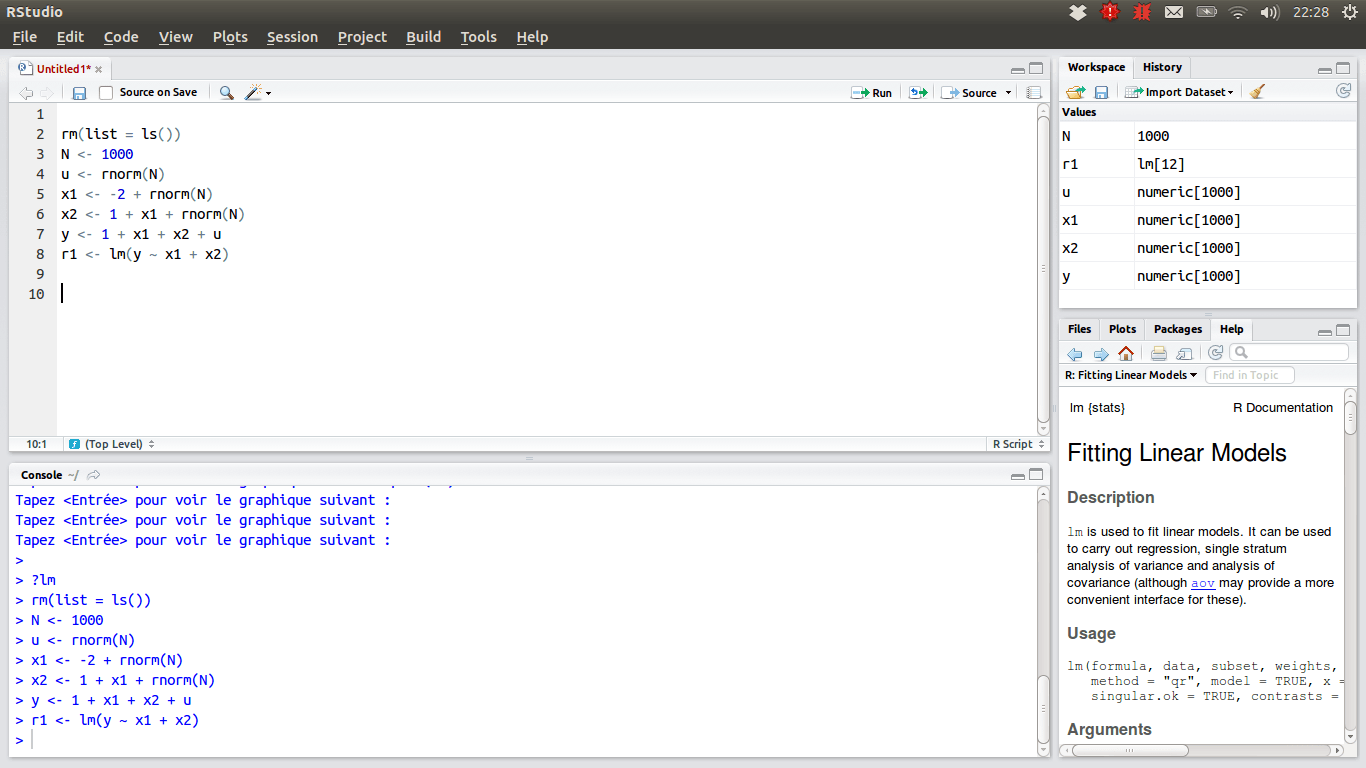
\includegraphics{images/rstudio.png}
\caption{\label{fig:"R"}}
\end{figure}

Para Phyton suele utilizarse Spyder y Jupyter Notebook. Las presentaciones de estos dos entornos son los siguientes:

Entorno de Spyder:

\begin{figure}
\centering
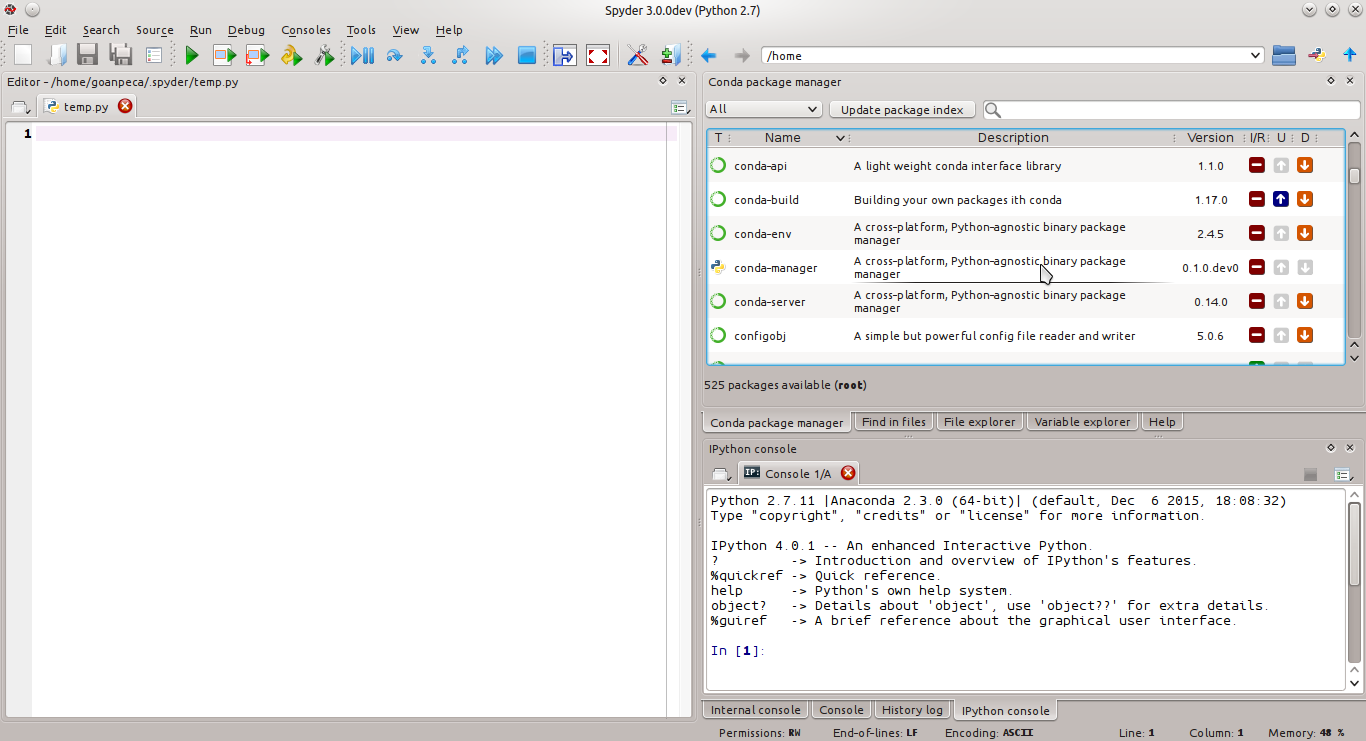
\includegraphics{images/spyder.png}
\caption{\label{fig:"spyder"}}
\end{figure}

Entorno de Jupyter notebook:

\begin{figure}
\centering
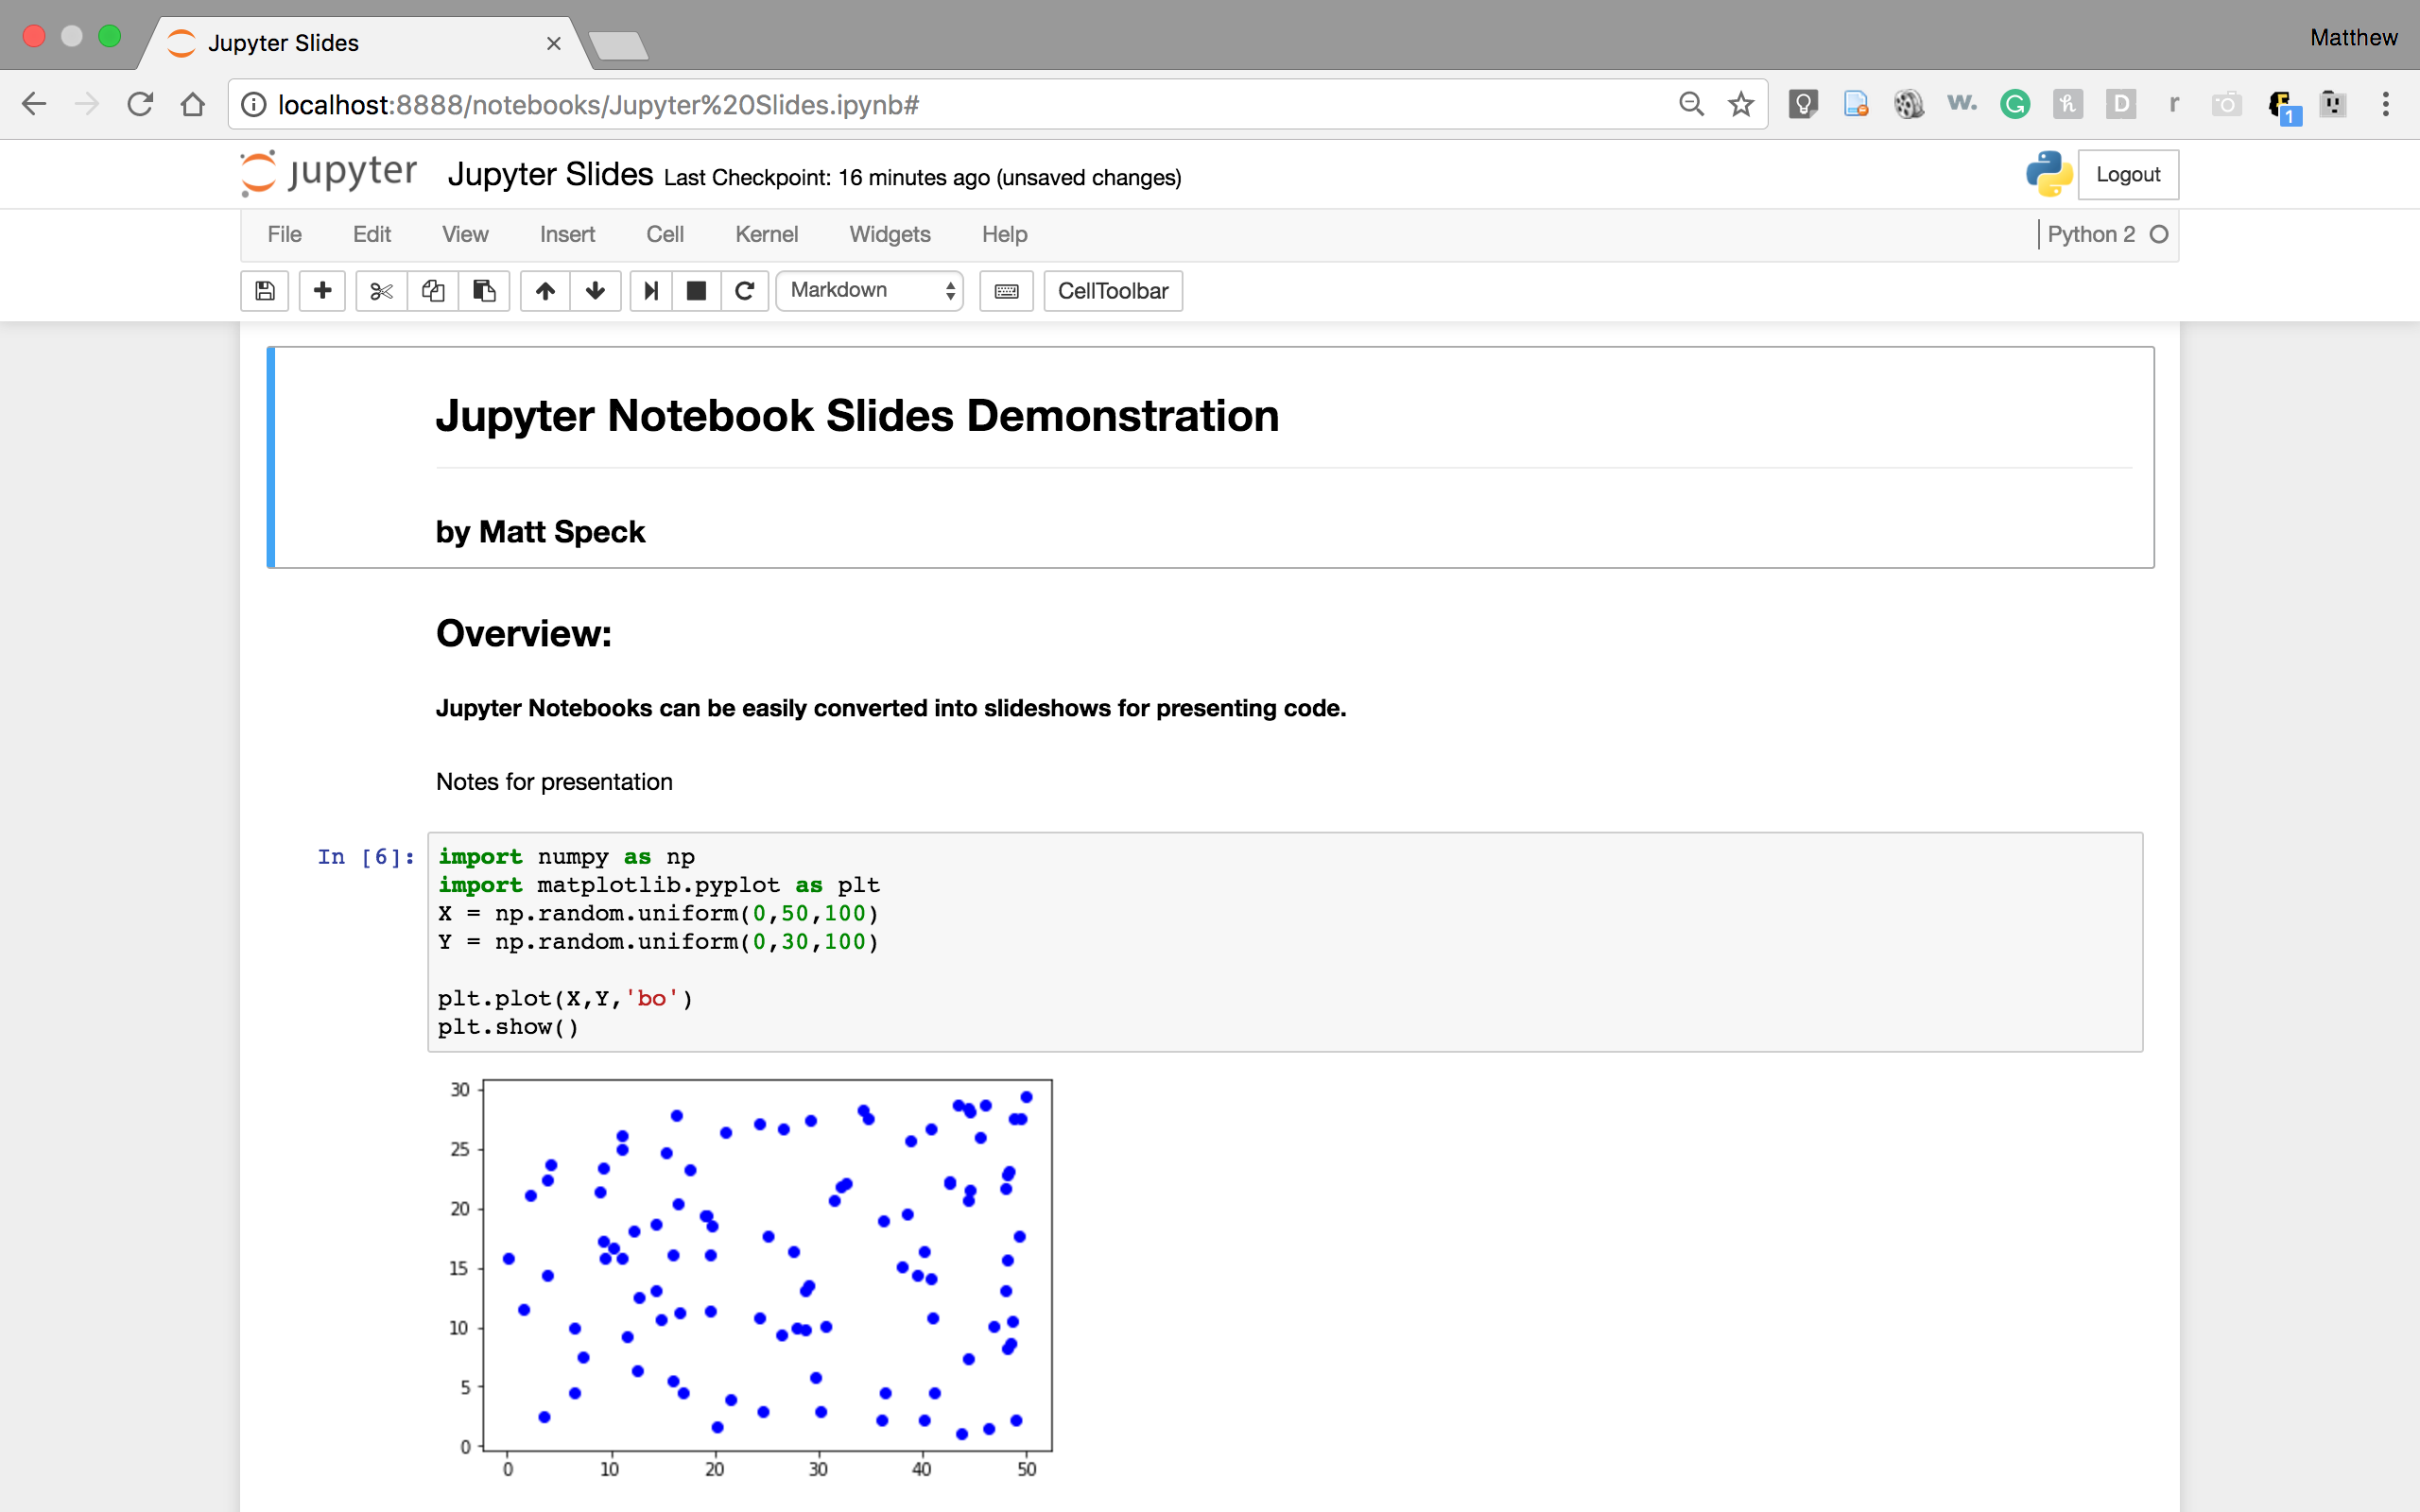
\includegraphics{images/jupyter.png}
\caption{\label{fig:"R"}}
\end{figure}

Aunque con estos entornos se nos facilita mucho el trabajo seguimos con el incoveniente de que muchas de las librerías para la ciencia de los datos debemos instalarlas por nuestra cuenta, este problema se solventa con la existencia de ambientes de desarrollo para científicos de datos que incluyan todos estos factores.

\hypertarget{anaconda}{%
\section{Anaconda}\label{anaconda}}

Anaconda es una distribución libre y abierta que incluye los lenguajes \emph{R} y \emph{Python} que permite a los científicos de datos poder trabajar de una manera mas comoda y centralizada. Ananconda trae por defecto una gran cantidad de librerías orientadas a la ciencia de datos y projectos de Machine Learning, ademas nos permite descargar \emph{Rstudio} con un simple clik. La presentacion que veremos cuando abramos \emph{Anaconda} es :

\begin{figure}
\centering
\includegraphics{images/Anaconda.png}
\caption{\label{fig:"R"}}
\end{figure}

Se recomienda el uso de Anaconda para el público en general, para los principiantes debido a que permite un rapido inicio sin tener que descargar programas y paquetes por su propia cuenta y de esta forma concentrarse en el aprendizaje y para los avanzados ya que permite un trabajo mas centralizado y eficiente al poder tener un ambiente con todo los requerimientos que se necesiten para poder trabajar de una forma mas comoda. \emph{Anaconda} se puede descargar en el siguiente enlace: \url{https://www.anaconda.com}

\hypertarget{librerias}{%
\section{Librerías}\label{librerias}}

A pesar de que al descargar Anaconda vienen por defecto una gran cantidad de librerías o paquetes, podríamos estar interesados en instalar alguno que tal vez no lo esté. En esta sección enseñaremos como instalar paquetes de forma rápida y sencilla.

\hypertarget{instalando-librerias-en-r}{%
\subsection{\texorpdfstring{Instalando librerías en \emph{R}}{Instalando librerías en R}}\label{instalando-librerias-en-r}}

Las descargas de las librerías en \emph{R} la haremos directamente desde \emph{RStudio}. Para ello hacemos clic en la pestaña \emph{Package } ubicadas en la sección inferior derecha subrayada en rojo, luego haremos clic en el botón \emph{Install}

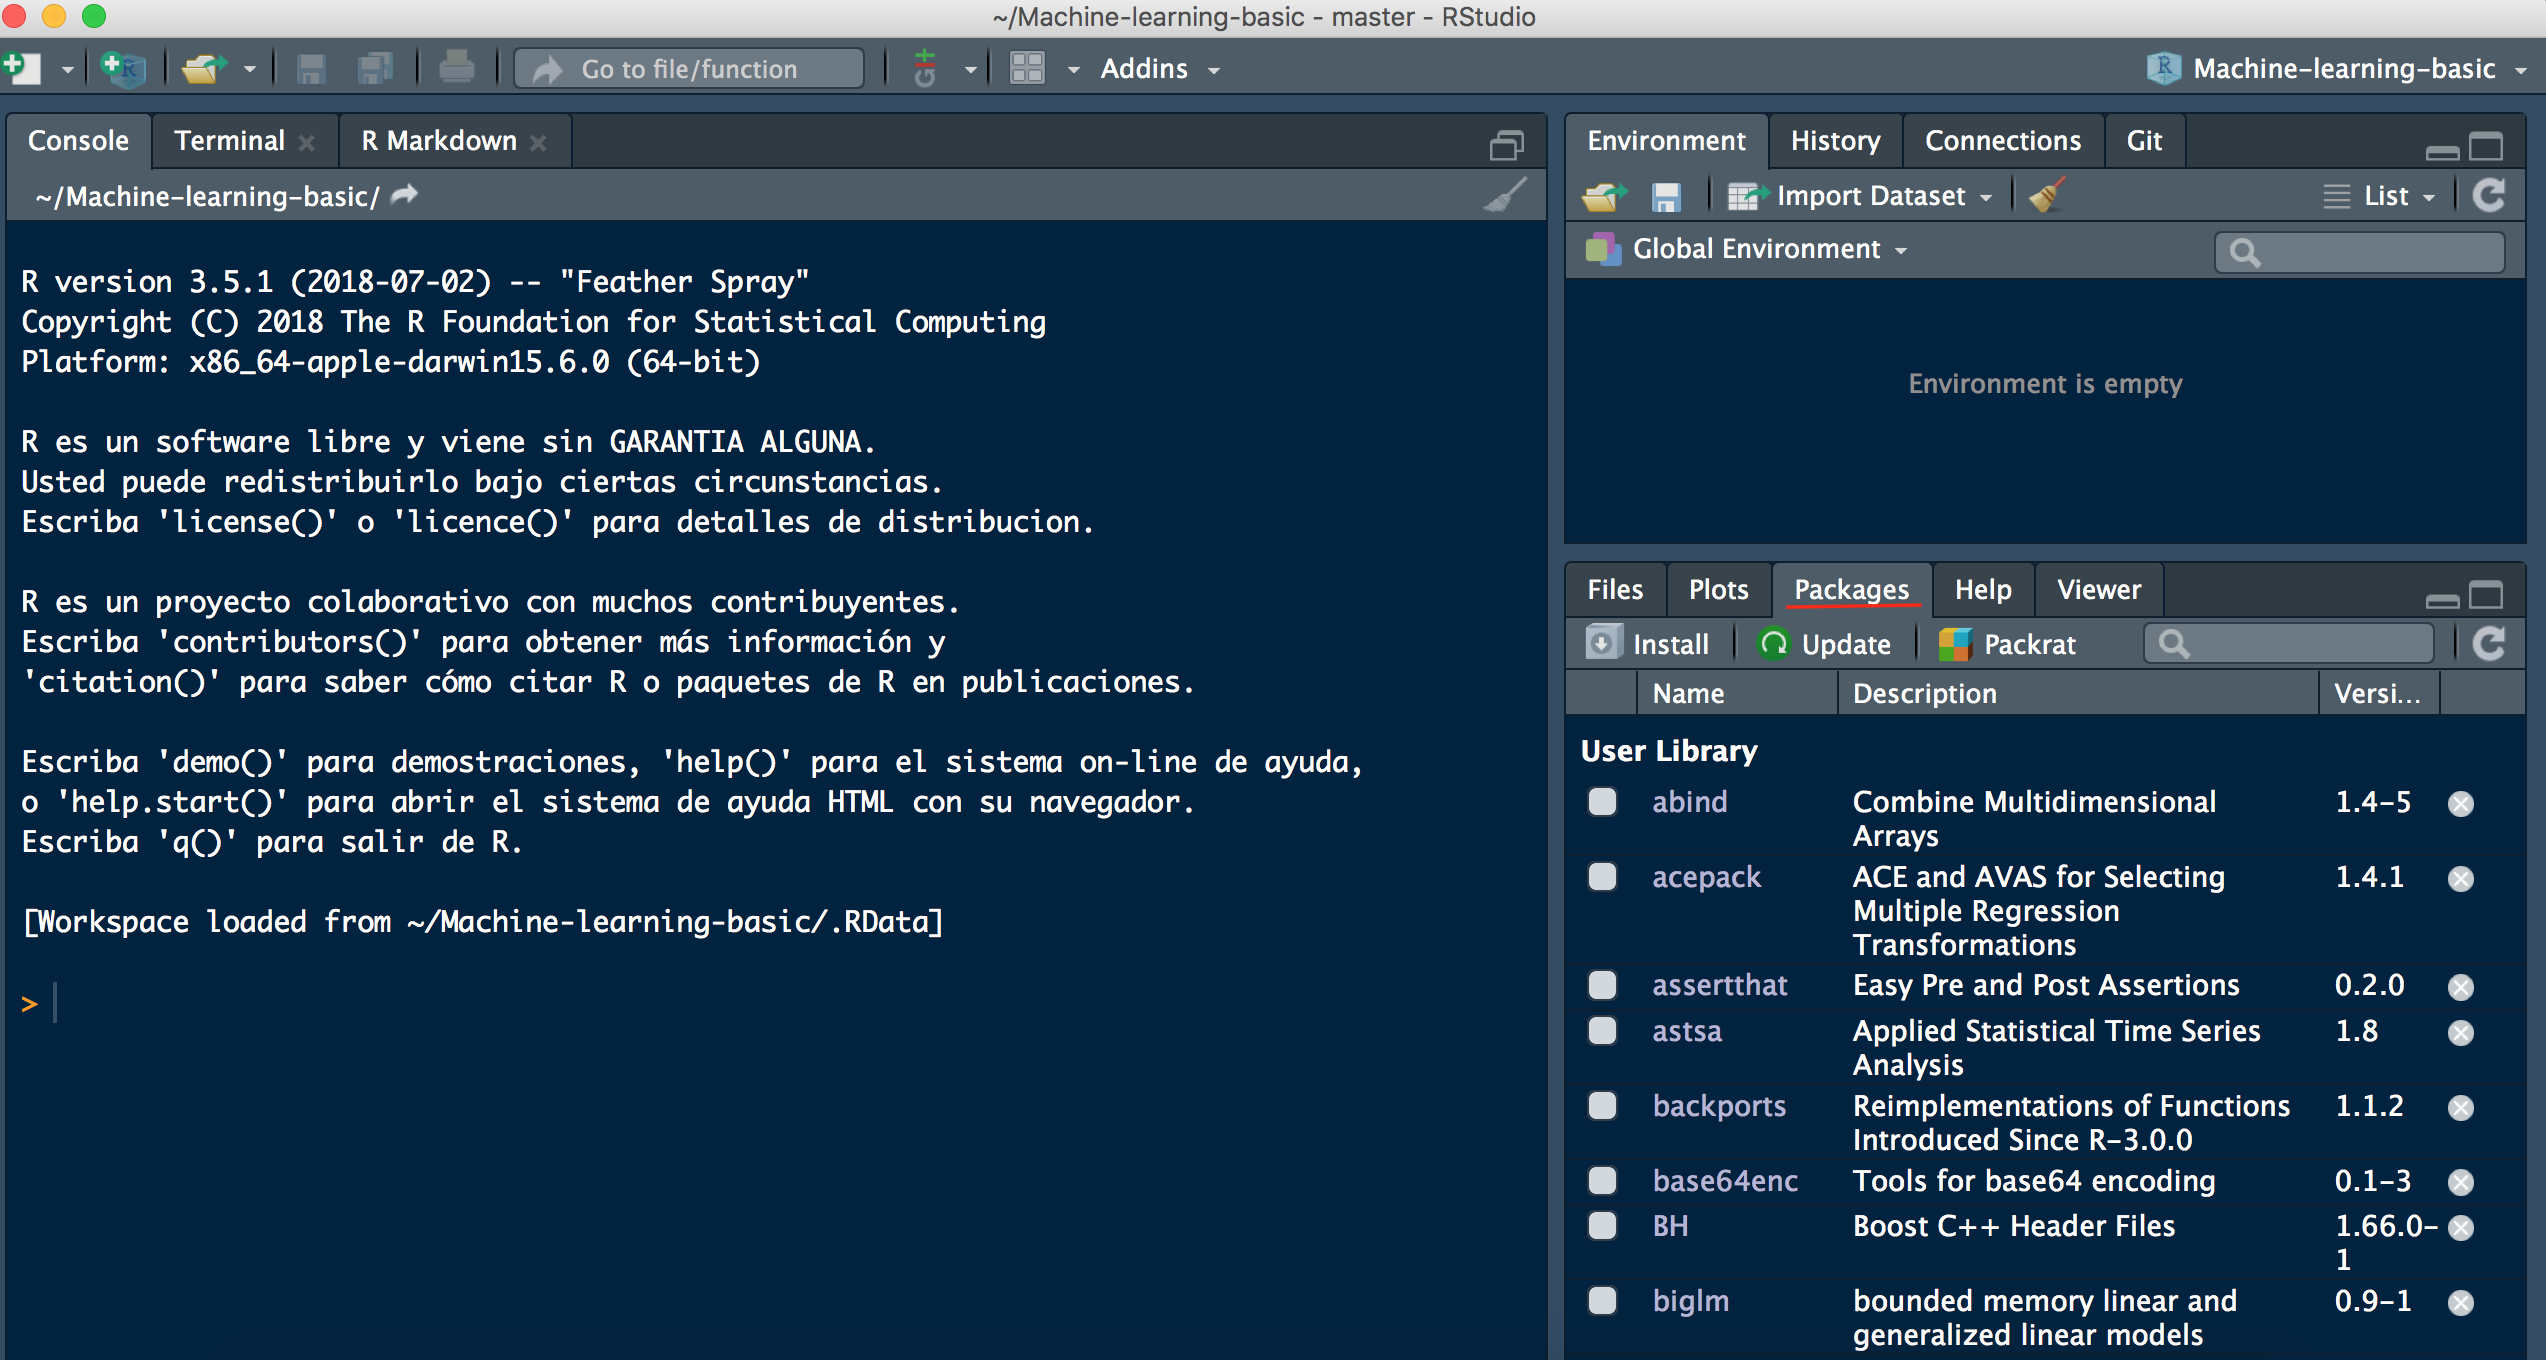
\includegraphics{images/packa1.png}
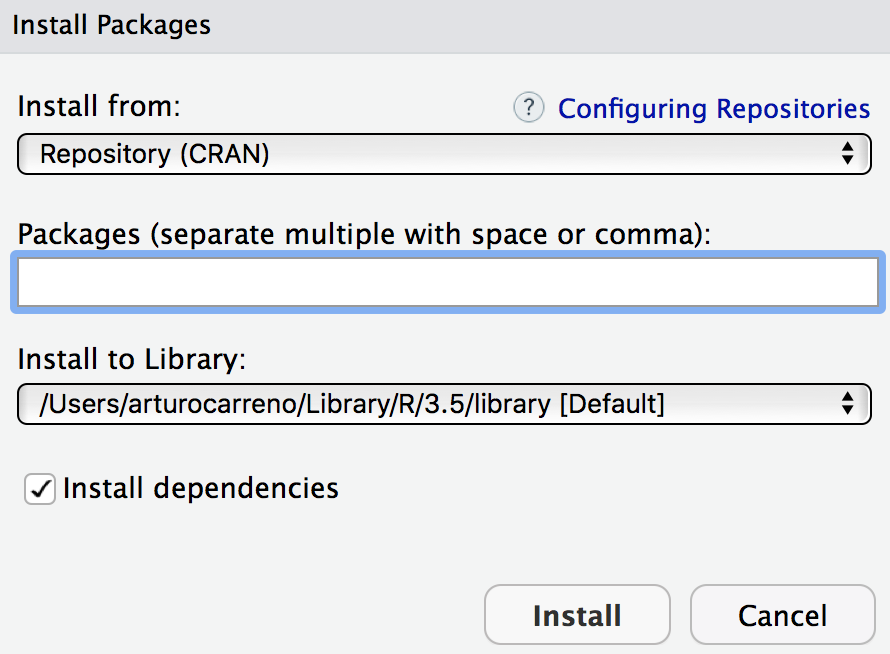
\includegraphics{images/packa2.png}

Los campos de información solicitada se refieren a:

\begin{itemize}
\item
  \emph{Install From}: Se utiliza para instalar paquetes desde la base de datos oficial de R o desde algún archivo específico. En este último caso es necesario indicar la ruta del archivo.
\item
  \emph{Package}: Debemos colocar el nombre del paquete que vamos a instalar. Si deseamos instalar varios paquetes a la vez, debemos colocar sus nombres y separarlos por comas o puntos y comas.
\item
  \emph{Install to library}: Ruta donde estará guardado el paquete una vez instalado. Se recomienda dejar el valor por defecto.
\item
  \emph{Install dependencies}: Algunos paquetes necesitan del uso de otros paquetes para su correcto funcionamiento. Al tildar esta opción estamos otorgándole permiso a RStudio para que instale las librerías que necesita el paquete que deseamos instalar.
\end{itemize}

\hypertarget{instalando-librerias-en-python}{%
\subsection{\texorpdfstring{Instalando librerías en \emph{Python}}{Instalando librerías en Python}}\label{instalando-librerias-en-python}}

Descargar librerías en \emph{Python} no es tan fácil como en \emph{R}, pero Anaconda facilita esta tarea. En el navegador de \emph{Anaconda} vamos a la sección \emph{Ambientes}, en inglés \emph{Environments}, y al lado del buscador seleccionamos la acción \emph{Todo}, \emph{All} en inglés, colocamos el nombre del paquete que deseamos instalar y se nos desplegará en la parte inferior derecha dos opciones: \emph{Aplicar} o \emph{Apply} y \emph{Borrar} o \emph{Clear}. Seleccionamos la opción \emph{Apply} y se instalará el paquete deseado.

\begin{figure}
\centering
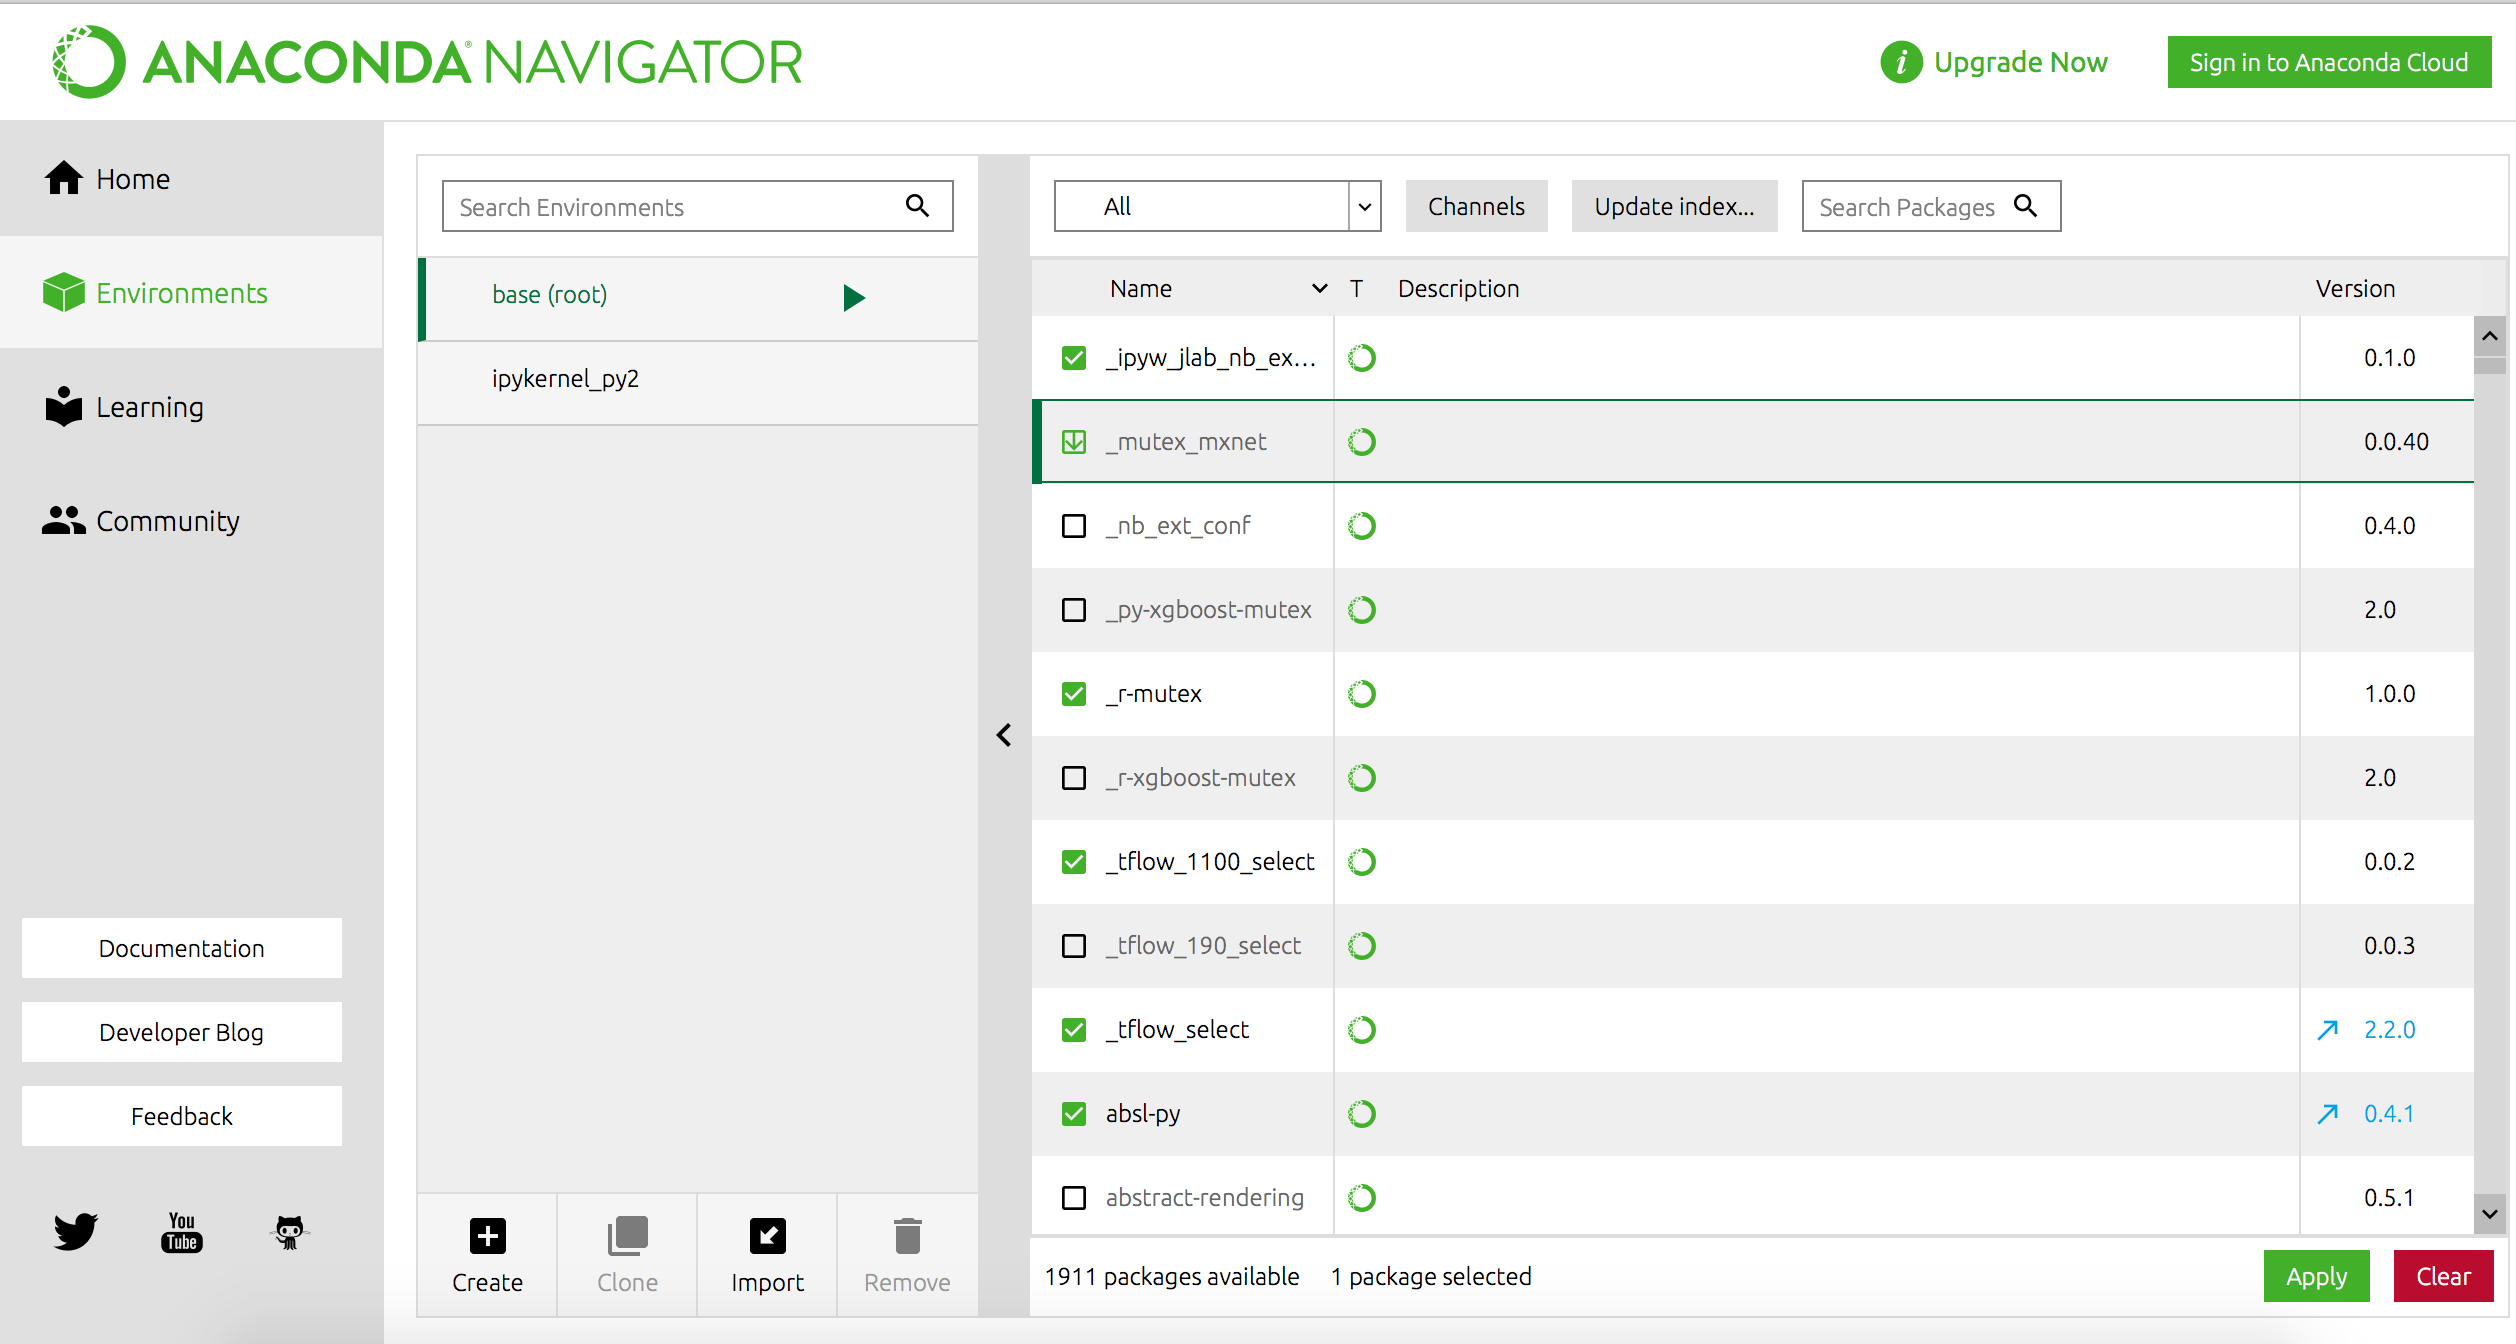
\includegraphics{images/packa3.png}
\caption{\label{fig:"R2"}}
\end{figure}

Si el paquete no está disponible en el ambiente tenemos la opción de instalarlo desde la terminal de \emph{Anaconda}. En la sección \emph{Environment} hacemos clic en la flecha al lado de la palabra base (root) y seleccionamos \emph{Open terminal}, tal como se muestra en la imagen

\begin{figure}
\centering
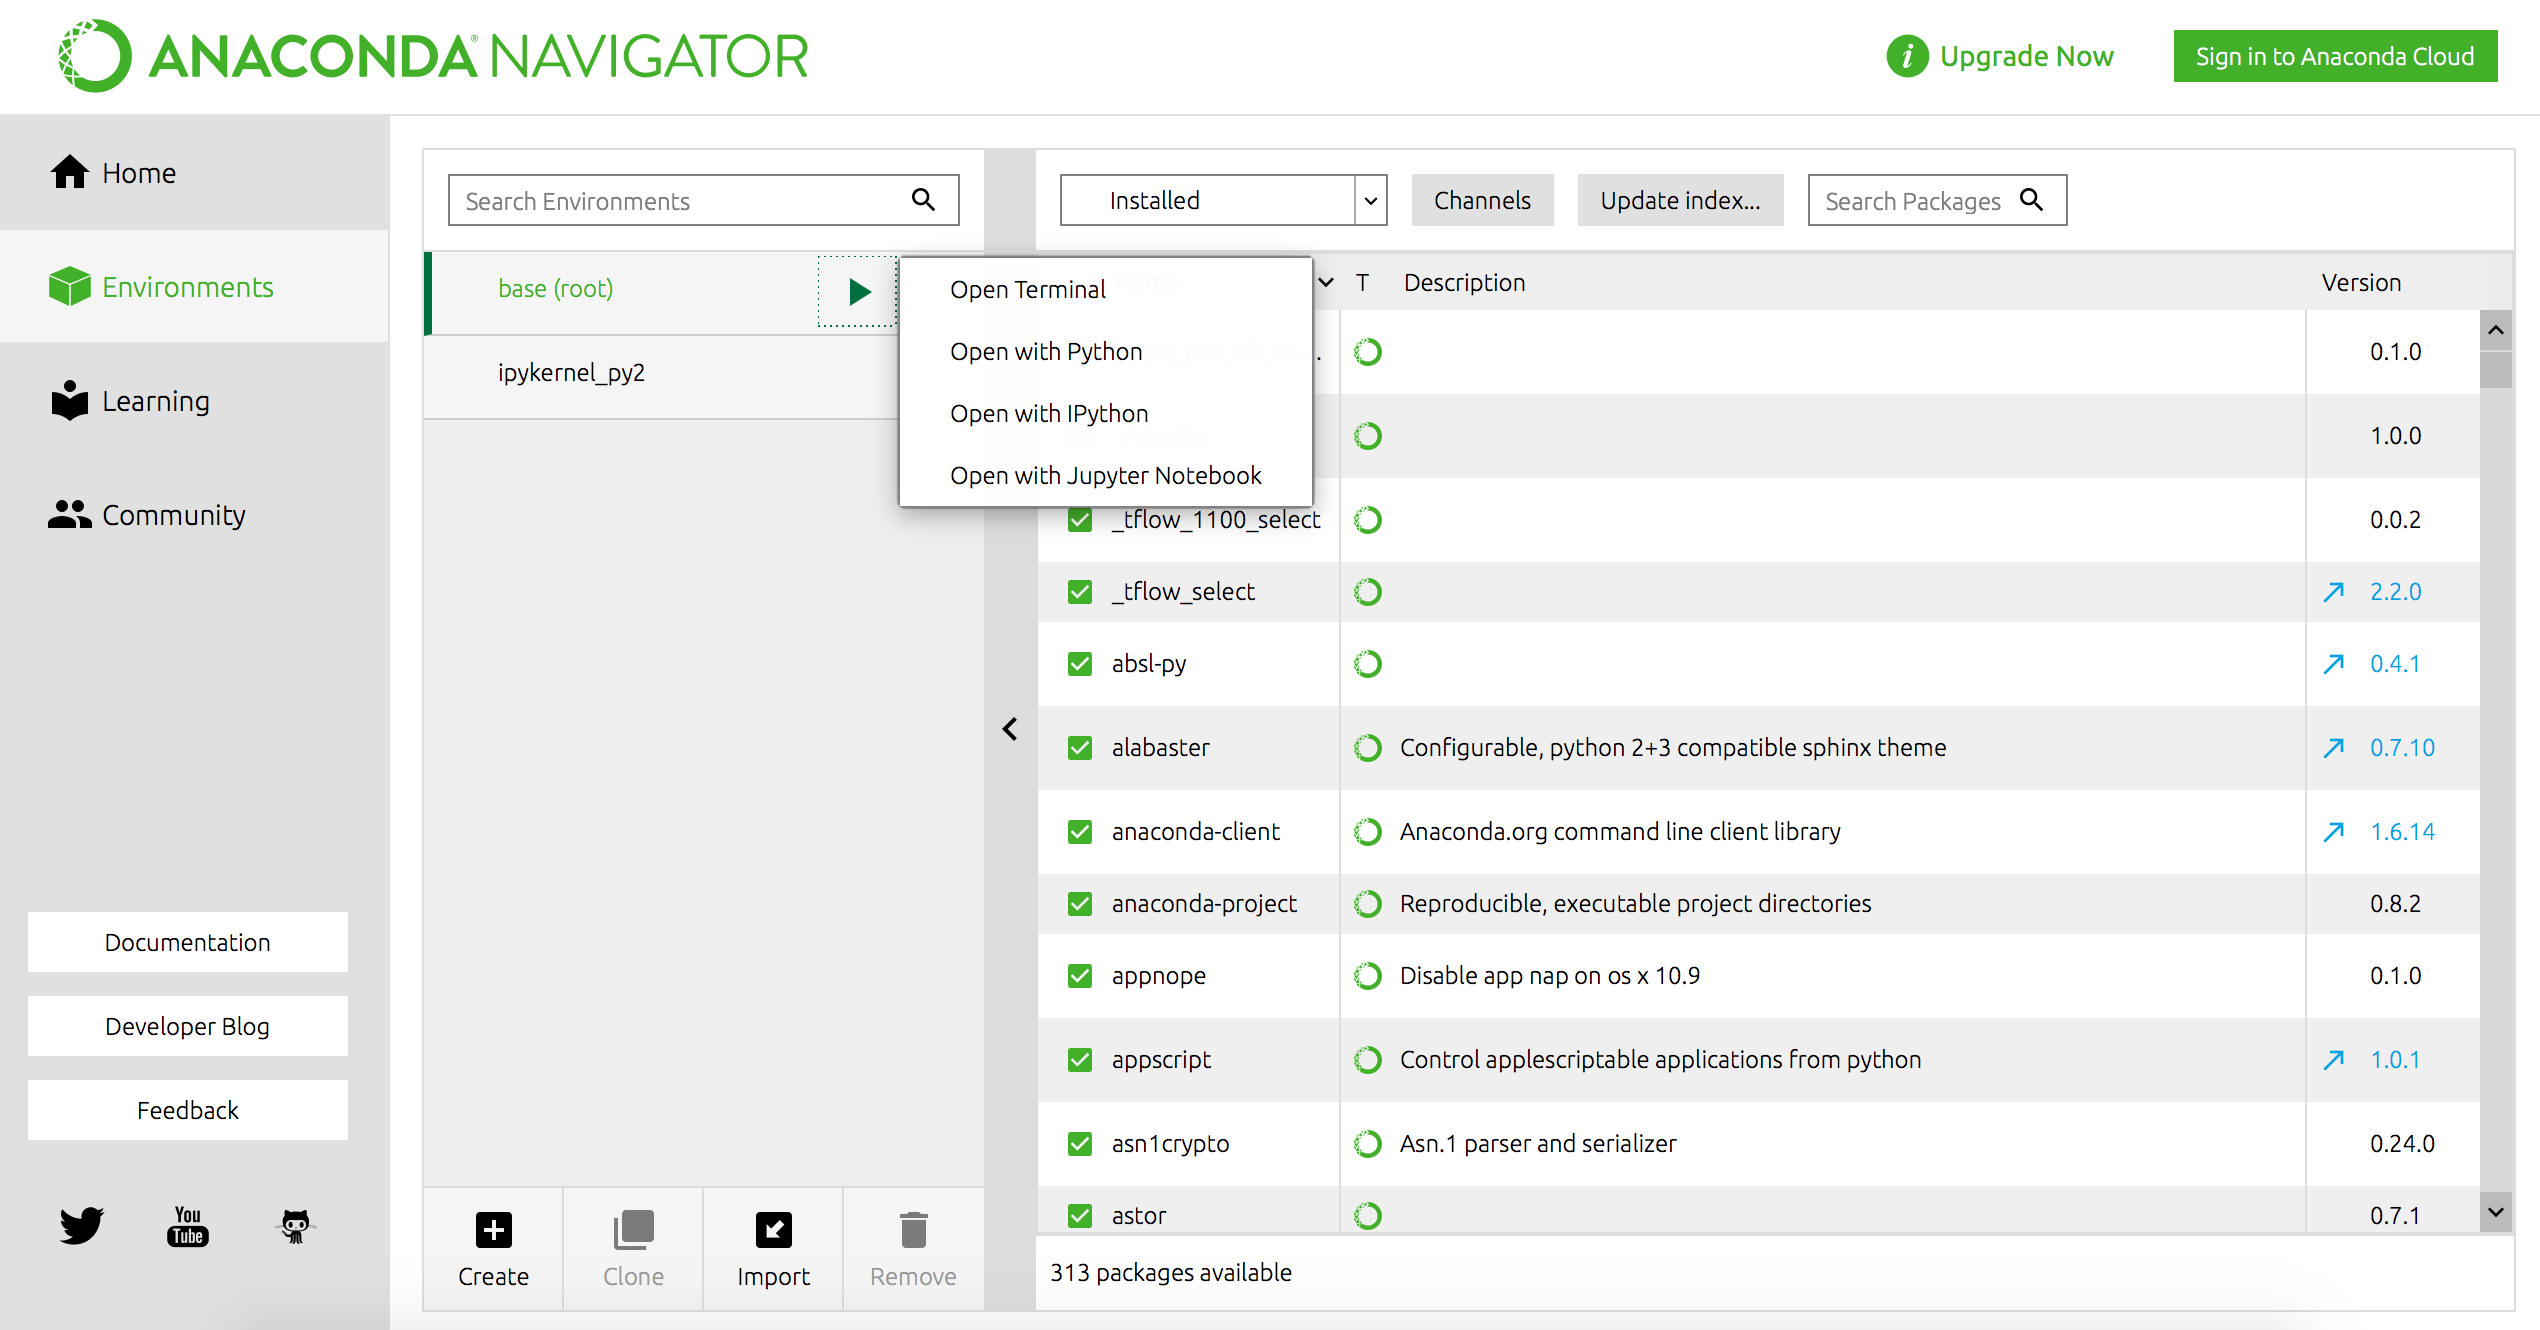
\includegraphics{images/packa4.png}
\caption{\label{fig:"R2"}}
\end{figure}

Se abre la consola del terminal y allí escribimos el comando \emph{conda install ``Nombre del paquete''} como se presenta a continuación

\begin{figure}
\centering
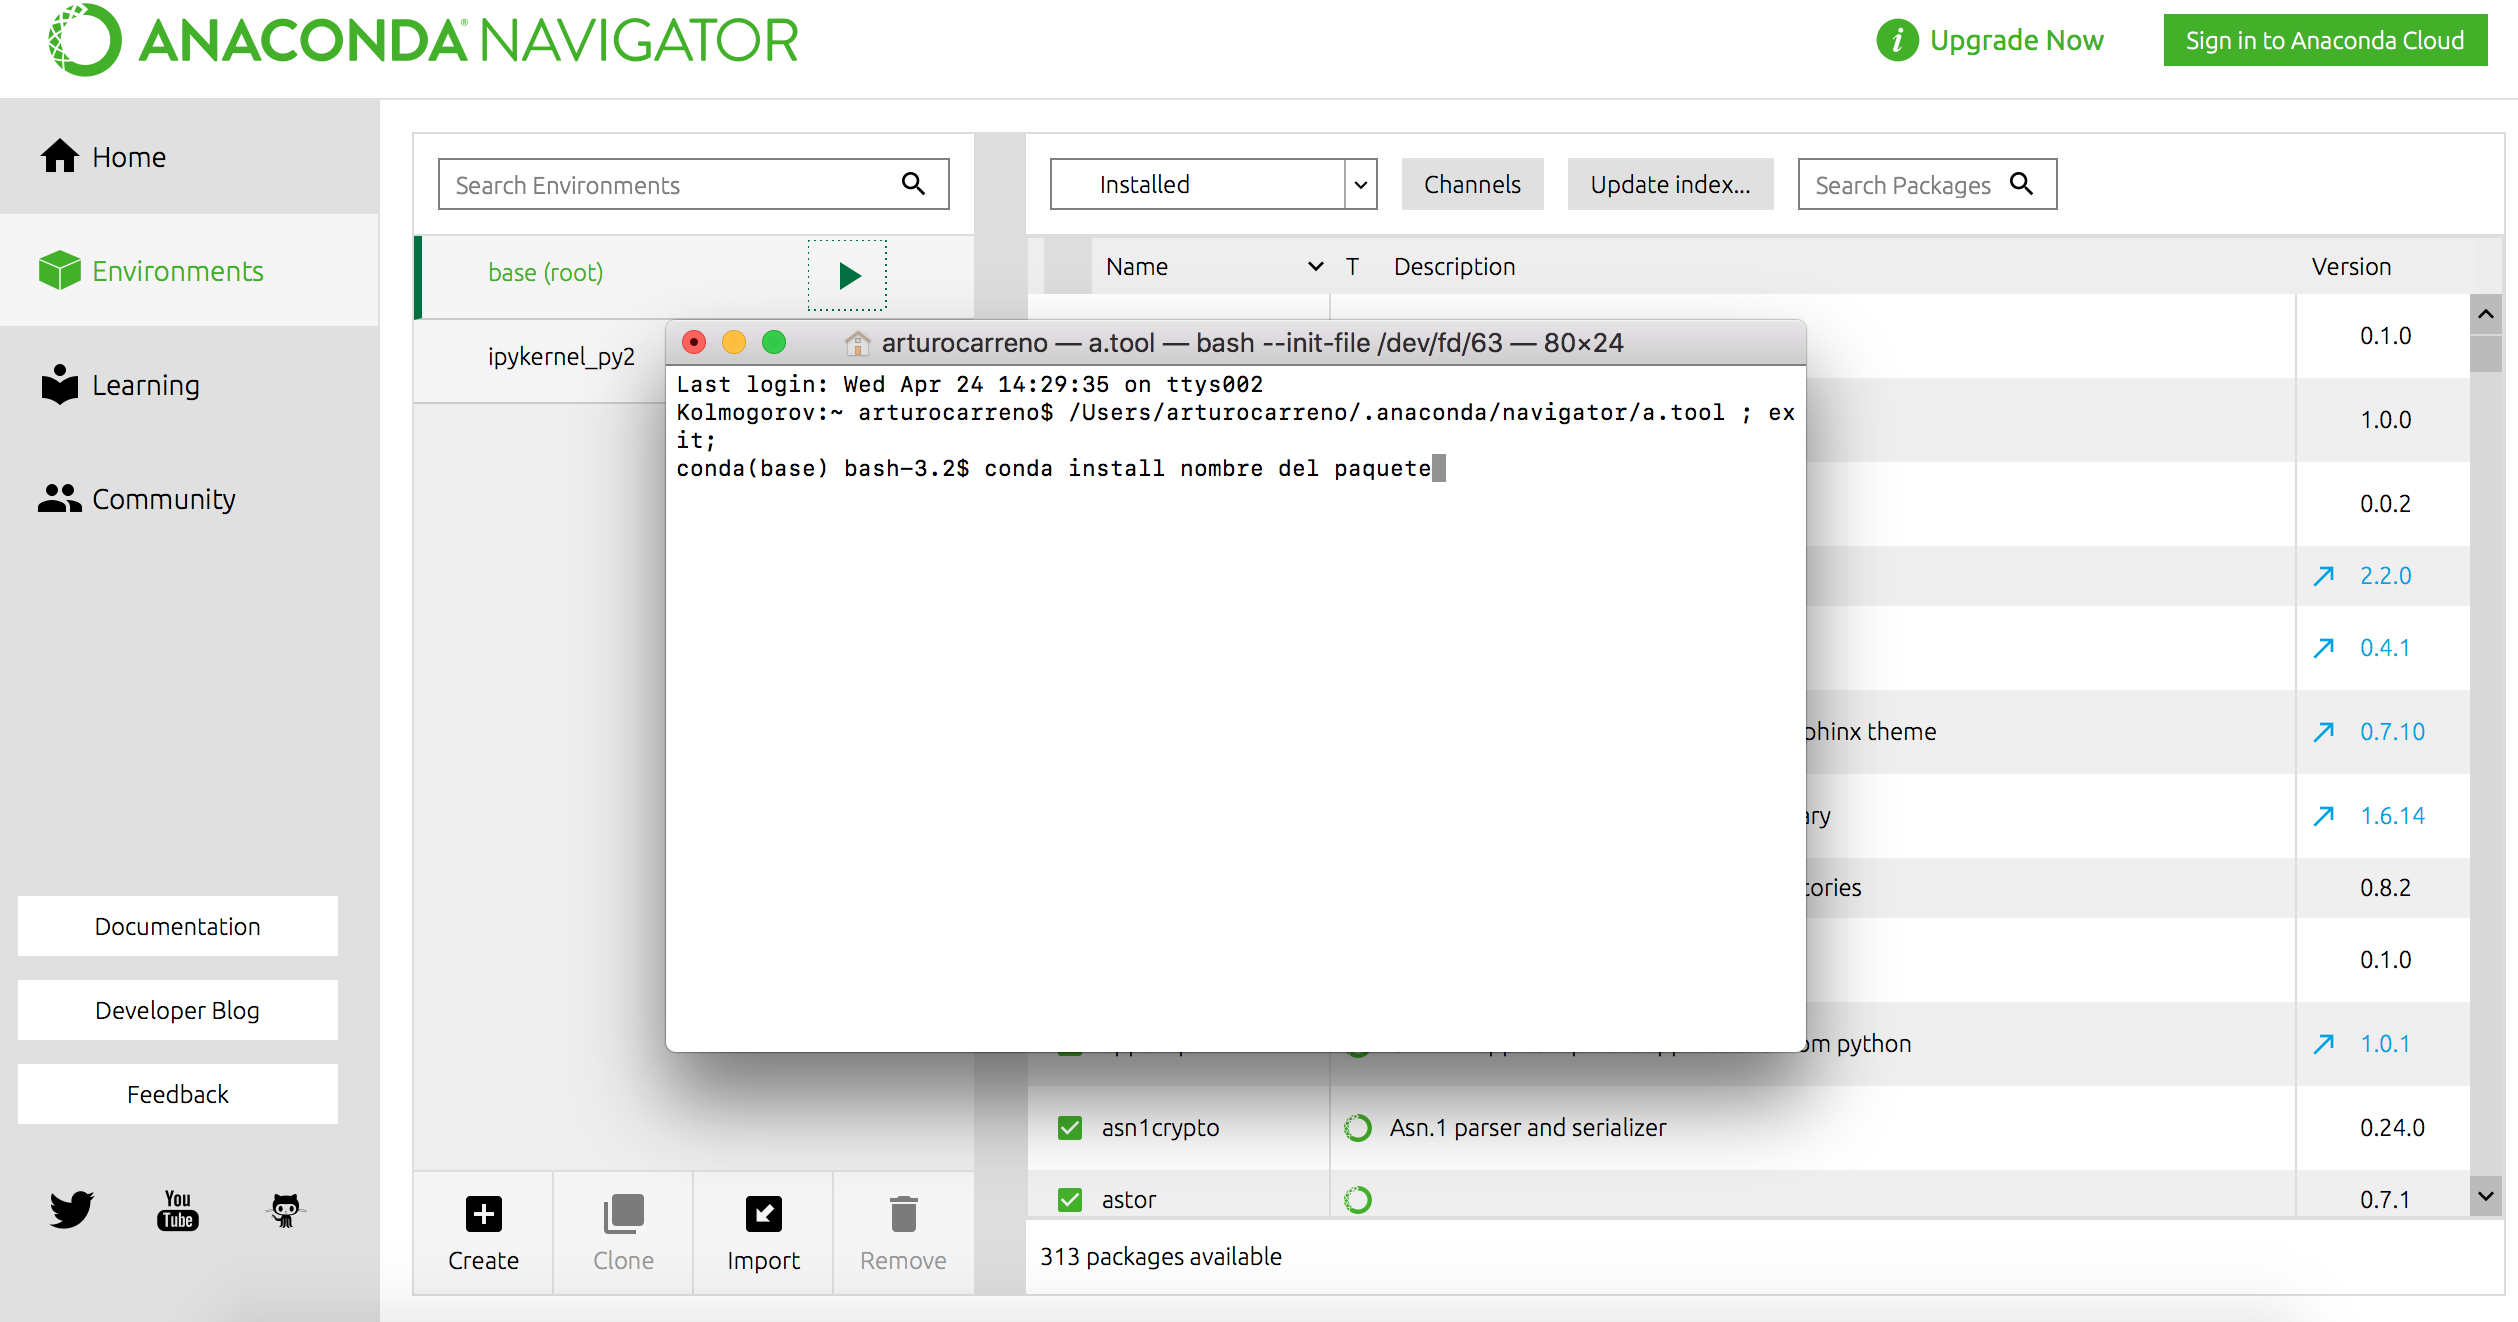
\includegraphics{images/packa5.png}
\caption{\label{fig:"R2"}}
\end{figure}

\hypertarget{uso-y-preparacion-de-los-datos}{%
\chapter{Uso y preparación de los datos}\label{uso-y-preparacion-de-los-datos}}

Al iniciar cualquier estudio debemos tener en cuenta que sin un buen conjunto de datos la mayoría de las técnicas que implementaremos darán resultados muy pobres. Si descuidamos la calidad de los datos, nuestros análisis se alejarán de la realidad que intentamos representar. La existencia de puntos atípicos, variables sin datos o con errores, pueden ser una verdadera pesadilla al iniciar nuestro estudio, por tal razón los lenguajes poseen herramientas que nos permiten manejar correctamente estas situaciones. En esta sección estudiaremos las herramientas básicas que \emph{R} y \emph{Phyton} ofrecen a todo analista que inicie un proyecto con datos con los cuales no esté familiarizado.

\hypertarget{lectura-de-datos}{%
\section{Lectura de datos}\label{lectura-de-datos}}

En general hay tres tipos de datos básicos con los cuales nos enfrentaremos, los cuales son archivos con extensiones \emph{.csv}, \emph{.txt}, \emph{xls}. Existen otras extensiones pero es muy raro que tenga que trabajar con datos provenientes de ellas, estas extensiones pueden ser: \emph{.docx}, \emph{.pdf}, entre otras

\hypertarget{lectura-de-datos-con-r}{%
\subsection{\texorpdfstring{Lectura de datos con \emph{R}}{Lectura de datos con R}}\label{lectura-de-datos-con-r}}

\emph{RStudio} nos facilita mucho esta tarea, pues tiene una opción que nos permite cargar los datos y escoger la configuracion del archivo sin tener que programar, veremos como hacer esto de forma directa y luego de manera adicional presentaremos algunas funciones que hacen esta misma tarea.

\begin{itemize}
\tightlist
\item
  Archivos \emph{csv} o \emph{txt}: Primero buscamos en las opciones que se encuentran disponibles en la parte superior de \emph{RStudio} y selecionamos \emph{archivo} o \emph{file}, luego se desplegaran varias opciones de las cuales debemos seleccionar \emph{Import Dataset} o \emph{importar datos}, recomendamos utilizar la opción \emph{From Text (readr)\ldots{}}, debido a su alta variedad de opciones para cargar los datos.
\end{itemize}

\begin{figure}
\centering
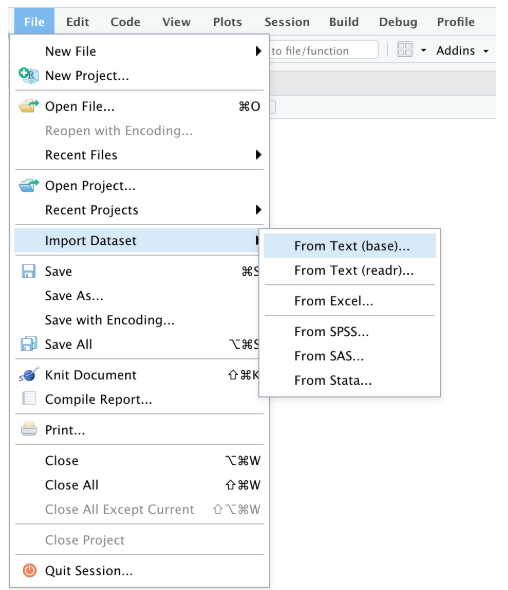
\includegraphics{images/dat.png}
\caption{\label{fig:"R2"}}
\end{figure}

El paquete \emph{readr} nos permite seleccionar las siguientes opciones

\begin{enumerate}
\def\labelenumi{(\roman{enumi})}
\item
  Cargar archivos directamente desde una ruta de nuestro computador o de una dirección web.
\item
  Seleccionar con un simple clic el tipo de datos de alguna columna en particular.
\item
  Mantener o eliminar columnas.
\item
  Cambiar el nombre al conjunto de datos.
\item
  No usar una cantidad \(N\) de las primeras filas del conjunto de datos.
\item
  Usar el encabezado como nombre de las columnas
\item
  Recortar espacios en los nombres
\item
  Cambiar los delimitadores de las columnas (separadas por comas, puntos y comas, tabulaciones, guiones, etc).
\item
  Seleccionar la codificación de los datos.
\item
  Identificar de alguna forma en particular los valores \emph{Na}
\end{enumerate}

\begin{figure}
\centering
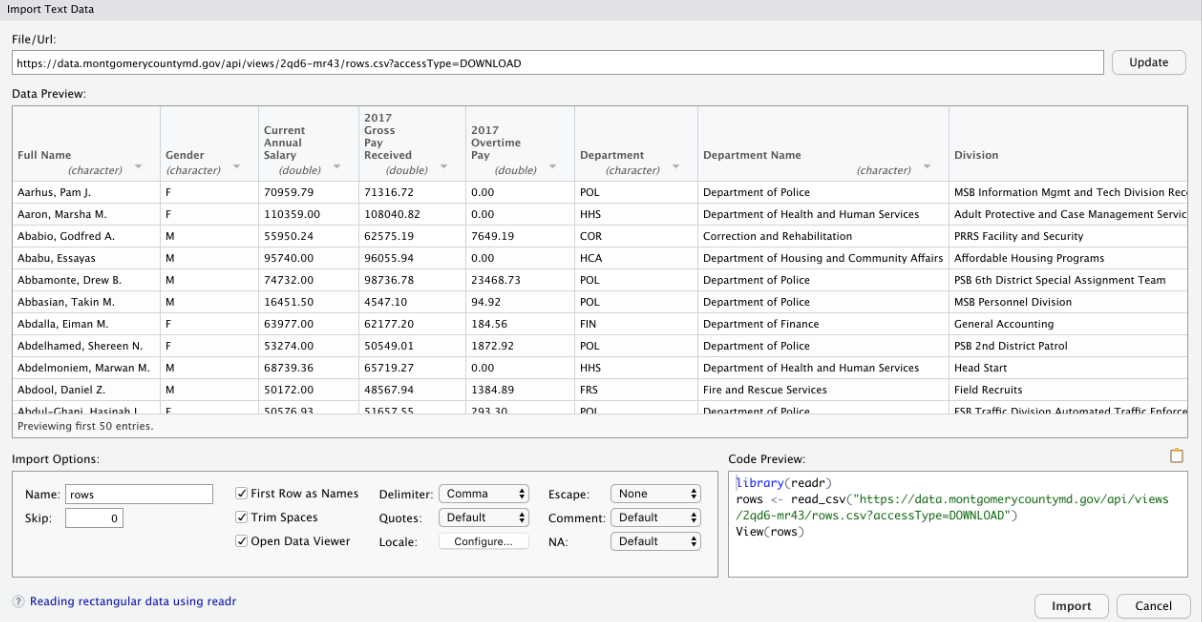
\includegraphics{images/dat1.png}
\caption{\label{fig:"R2"}}
\end{figure}

\begin{itemize}
\tightlist
\item
  Archivos \emph{.xls (MS-Excel)}: Para cargar archivos \emph{.xls} debemos seleccionar la opción \emph{From Excel} que se encuentra en la misma ubicación de las anteriores. Ésta opción usa el paquete \emph{readxl}. La ventaja de este paquete es que posee prácticamente las mismas opciones que los paquetes de \emph{R} básico para importar archivos de \emph{Excel}, pero además permite seleccionar la hoja de cálculo a usar del documento \emph{Excel}. La siguiente imagen representa lo que en general encontraremos al cargar un archivo \emph{Excel}:
\end{itemize}

\begin{figure}
\centering
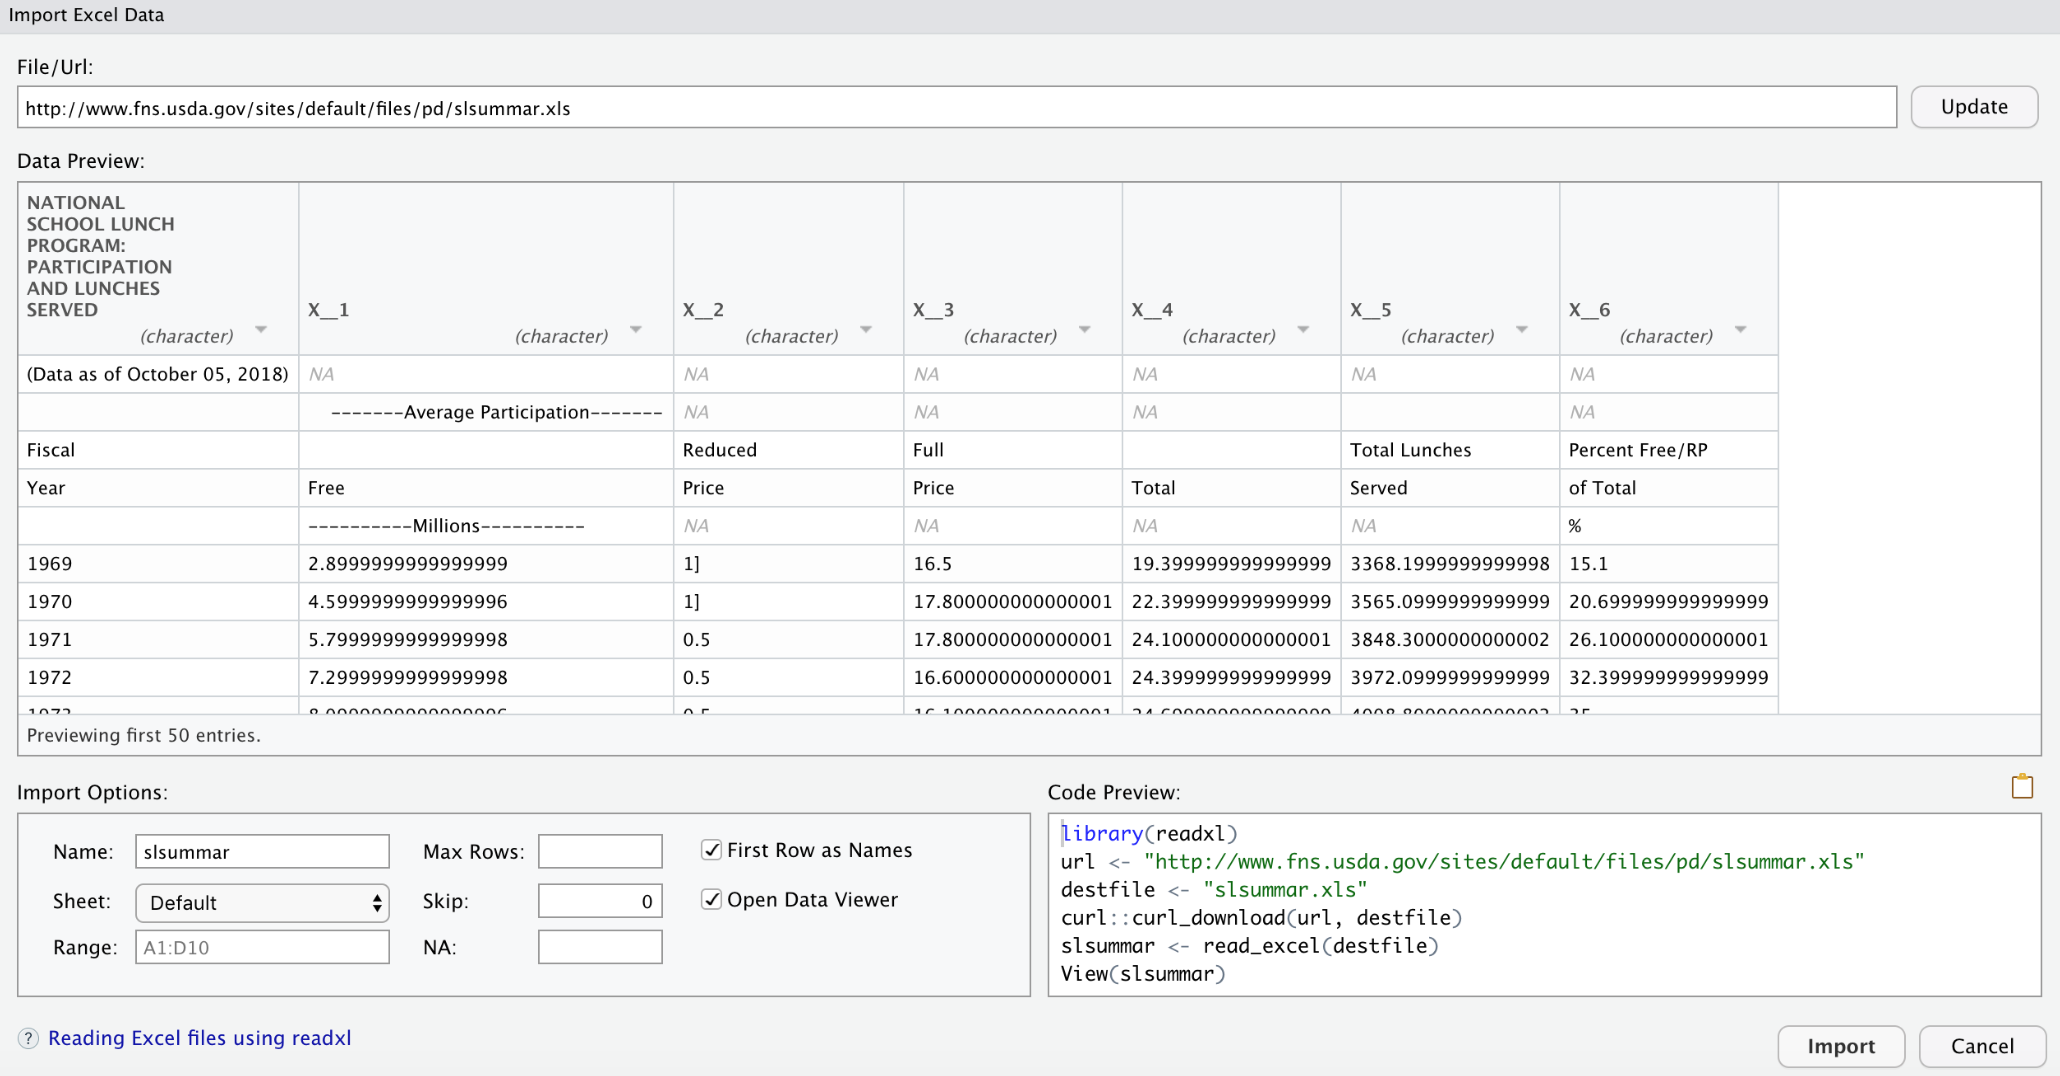
\includegraphics{images/dat3.png}
\caption{\label{fig:"R2"}}
\end{figure}

Gracias a \emph{readxl} podemos simplificar y mejorar los datos, en la variable \emph{skip} se coloca un valor numérico para indicar cuantas de las primera lineas se deben eliminar. Dando clic derecho sobre la variable número 3 cambiamos el tipo que trae por defecto. A continuación se muestra la imagen.

\begin{figure}
\centering
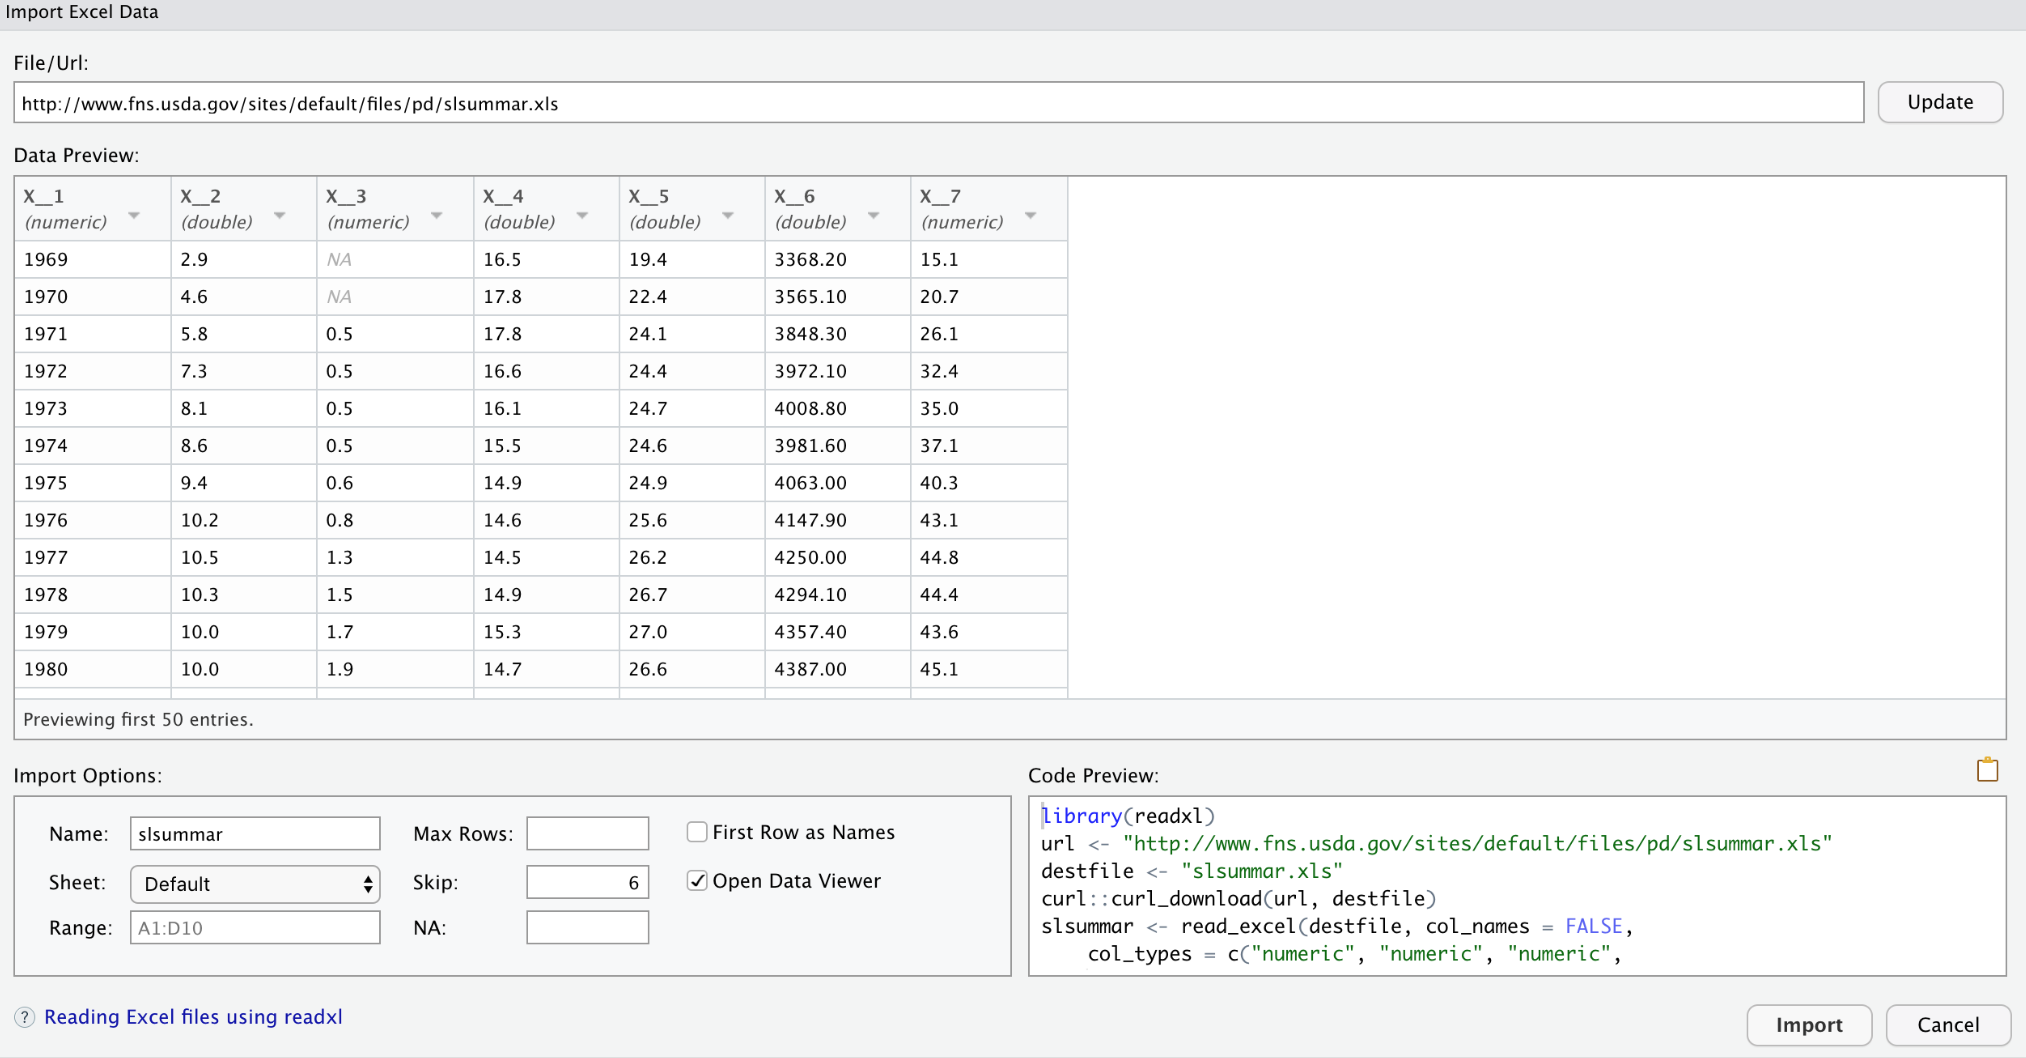
\includegraphics{images/dat4.png}
\caption{\label{fig:"R2"}}
\end{figure}

La importación de datos CSV o TXT puede hacerse directamente desde el R básico con paquetes especialmente diseñados para esta tarea como se muestra en el Apéndice.

\hypertarget{lectura-de-datos-con-python}{%
\subsection{\texorpdfstring{Lectura de datos con \emph{Python}}{Lectura de datos con Python}}\label{lectura-de-datos-con-python}}

La variedad de propósitos para los cuales se usa el lenguaje Python ha conducido a la existencia de una gran cantidad de formas de leer archivos \emph{.csv}, \emph{.txt}, \emph{.xlx}. Sin embargo la gran mayoría de los especialistas en Machine Learning que utiliza este lenguaje, optan por la librería \emph{Pandas} para la manipulación de datos. Por esta razón usaremos la funciones que nos ofrece \emph{Pandas}: \emph{pandas.read\_csv()} y \emph{pandas.read\_excel()}.
Ambas funciones aceptan una gran cantidad de parámetros, pero solo mencionaremos los más importantes. Una información mas detallada sobre estas funciones pueden encontrarse en:

\begin{itemize}
\item
  \url{https://pandas.pydata.org/pandas-docs/stable/reference/api/pandas.read_csv.html}
\item
  \url{https://pandas.pydata.org/pandas-docs/stable/reference/api/pandas.read_excel.html}
\end{itemize}

A diferencia de \emph{RStudio} no hay una forma en común para cargar los archivos, sin que tengamos que escribir algunas líneas de código. A continuación mostraremos como hacerlo:

\begin{itemize}
\item
  filepath\_or\_buffer: Ruta del archivo o dirección web.
\item
  Sep: valor que separa los datos, por defecto es una coma
\item
  header: Se usa para identificar en que posición se encuentra la fila que será usada como los nombres de las columnas.
\item
  \emph{names}: Lista con el nombre de las columnas a usar.
\item
  \emph{index\_col}: Columna que será usada por defecto como índice
\item
  \emph{decimal}: Carácter que será usado como carácter decimal, por defecto es un punto
\item
  \emph{usecol}: Este parámetro nos permite decidir qué número de columnas usar.
\item
  \emph{dtype}: Tipo de dato de cada columna, por ejemplo \{`a': np.float64, `b': np.int32, `c': `Int64'\}.
\end{itemize}

\begin{figure}
\centering
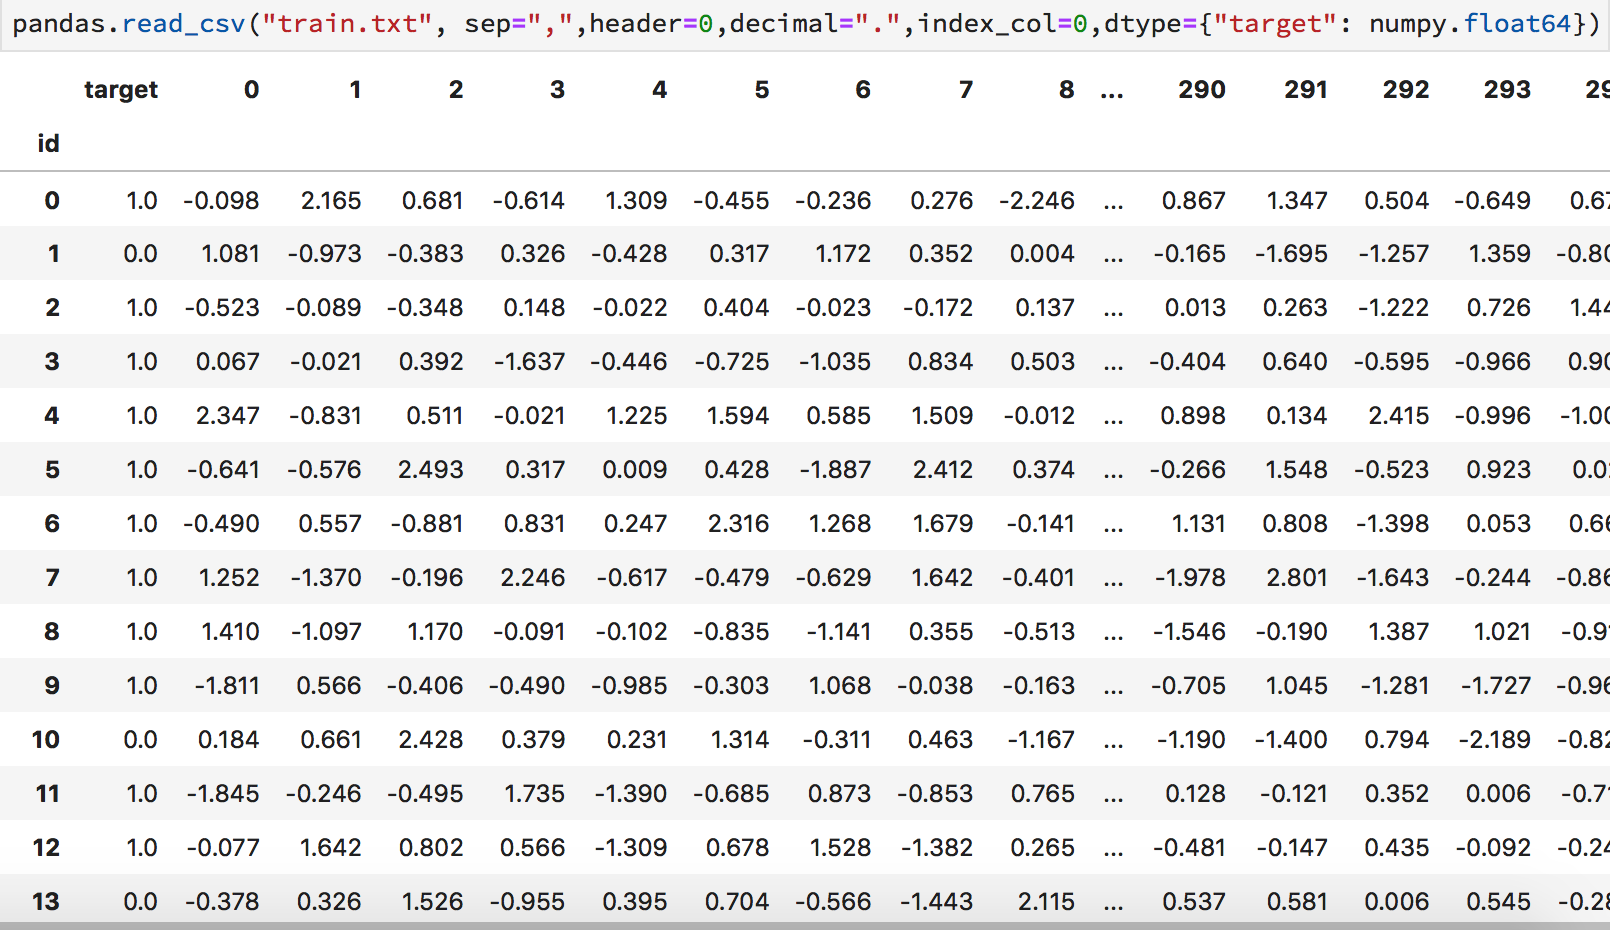
\includegraphics{images/dat5.png}
\caption{\label{fig:"R2"}}
\end{figure}

\begin{enumerate}
\def\labelenumi{(\roman{enumi})}
\setcounter{enumi}{1}
\tightlist
\item
  Leer archivos .\emph{xlx} con \emph{pandas.read\_excel()}: Usa prácticamente los mismos parámetros que la función anterior, con la diferencia de que no acepta el parámetro \emph{sep} y usa un parámetro adicional llamado \emph{sheet\_name}, este parámetro debe ser una lista con los números de columnas a usar o con los nombres de dichas columnas.
\end{enumerate}

\hypertarget{tratamiento-previo-de-los-datos}{%
\section{Tratamiento previo de los datos}\label{tratamiento-previo-de-los-datos}}

Luego de cargar los datos puede empezar la verdadera pesadilla para aplicar los métodos, debido a factores como errores de medición, problemas de codificación y errores humanos. En general clasificaremos estos problemas en dos grupos: \emph{Valores Faltantes} o \emph{Missing Values} y \emph{Valores Atípico} más conocidos por el término en inglés \emph{Outliers}.

\hypertarget{missing-values-o-valores-faltantes}{%
\subsection{Missing Values o valores faltantes}\label{missing-values-o-valores-faltantes}}

Estos valores suelen generarse por diversas razones, entre las cuales se encuentran: problemas de codificación con los datos, errores de medición y errores humanos, entre otros. En algunos casos pueden generarse por problemas con la función que esté encargada de leer los datos, sea porque no lee bien los parámetros o simplemente por incompatibilidad del archivo. En esta sección veremos cuáles son las técnicas más usuales para solucionar estos problemas.

\begin{enumerate}
\def\labelenumi{(\roman{enumi})}
\tightlist
\item
  Missing values en \emph{R}: Para trabajar con datos faltantes en \emph{R} lo primero es contarlos. Para ello usaremos la función \emph{sapply()} la cual permite aplicar funciones a columnas de manera explícita. En nuestro caso aplicaremos la función \emph{is.na()} la cual cuenta la cantidad de valores faltantes por columnas, la función \emph{sum()} que suma todos estos valores y nos da el resultado final, y la función \emph{dim()} la cual nos da las dimensiones de los datos.
\end{enumerate}

\begin{figure}
\centering
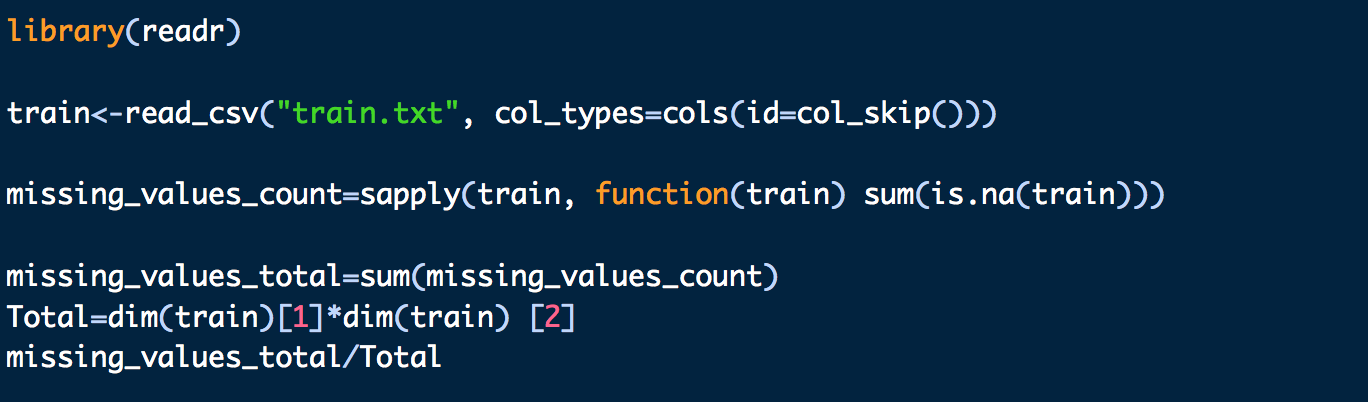
\includegraphics{images/dat9.png}
\caption{\label{fig:"R2"}}
\end{figure}

En general, los valores faltantes tienden a eliminarse, pero esto no se puede hacer a la ligera, en otros casos suelen sustituirse por un valor común del conjunto de datos (esto se hace cuando tenemos distintas entradas para un individuo y alguna característica está vacía). También se debe chequear si la distribución de datos faltantes es aleatoria. Sería muy extraño que cada 100 datos exactamente exista un dato faltante en un lugar en específico. Este último tipo de comportamiento hace pensar en que estamos en presencia errores sistemáticos.

Como tratar estos casos, dependerá de nuestros propósitos específicos, pues los datos faltantes tienden a sesgar de manera considerable muchas técnicas estadísticas. Cuando elegimos no usarlos decimos que los eliminaremos y cuando optamos por sustituirlos por un valor en específico diremos que los imputaremos.
Para eliminar los datos faltantes sin riesgo a perder información vital, lo primero que debemos asegurarnos es que la proporción de estos datos con el total sea muy bajo, por ejemplo 300:1, si los valores faltantes representaran el 1\% de la población no es muy recomendable que los eliminemos. Un ejemplo típico es que pudieran representar un segmento de la población que por problemas de medición o de transmisión de los datos, simplemente no se pudo completar el llenado de información y el eliminarlos pudiera dejar por fuera una parte importante de la población. El 1\% no parece significativo, pero si tenemos 3 millones de datos el 1\% representaría 30 mil, una cantidad considerable, de posibles consumidores para un producto en específico.

Para eliminar los valores faltantes de la data por filas, usamos la función \emph{na.omit()}, si queremos eliminar por columnas usamos la función \emph{t()} la cual nos traspone los datos, el problema es que modificará el índice. Solventamos este problema con la función \emph{rownames()}. Otro detalle es que la función \emph{na.omit()} cambia el formato de los datos, por lo que usaremos la función \emph{as.data.frame()} para corregir el problema.

\begin{figure}
\centering
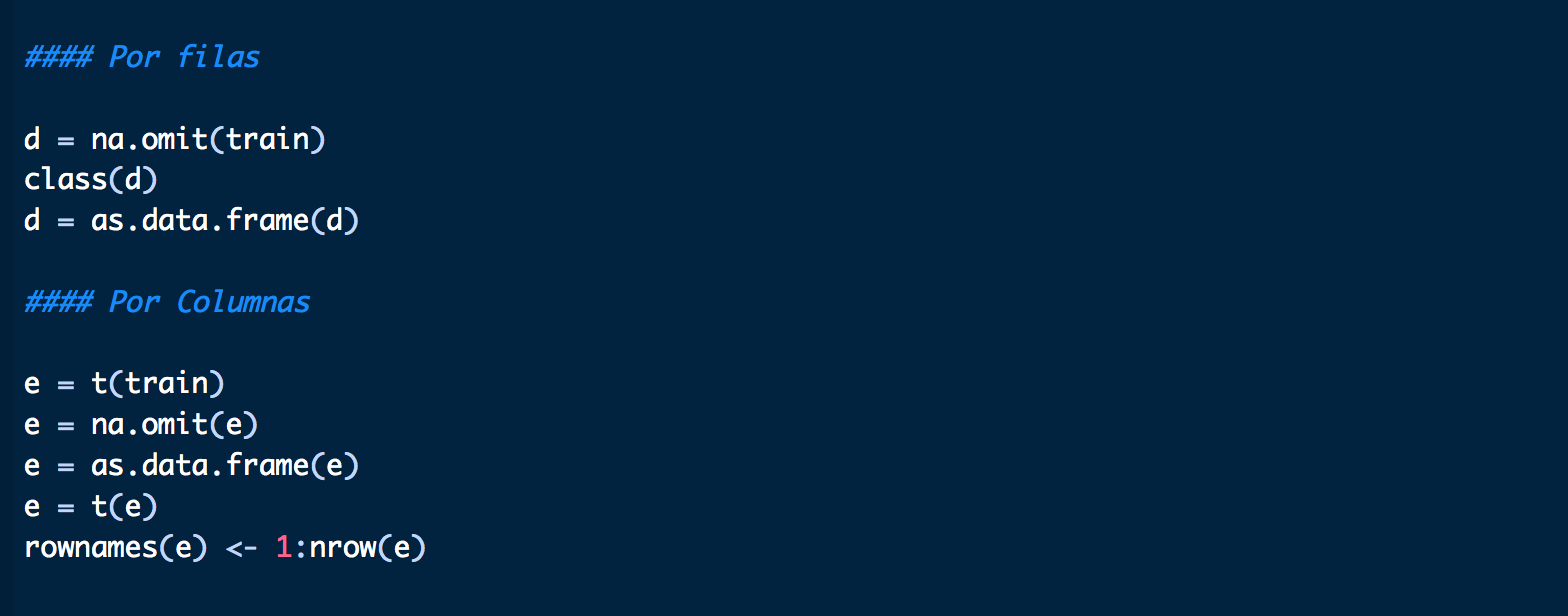
\includegraphics{images/dat10.png}
\caption{\label{fig:"R2"}}
\end{figure}

\begin{itemize}
\tightlist
\item
  Sustitución por la media: Cuando los datos poseen un comportamiento uniforme alrededor de una región del plano se suelen sustituir por el valor medio que presentan los datos.
\end{itemize}

\begin{figure}
\centering
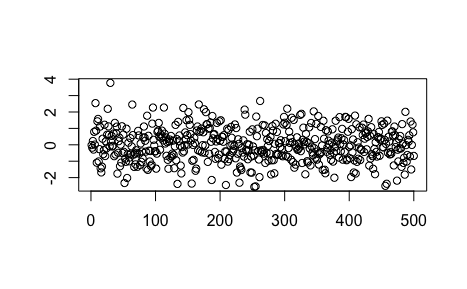
\includegraphics{images/Rplot.png}
\caption{\label{fig:"R2"}}
\end{figure}

Para sustituir por el valor medio se utiliza la función \emph{mean()} para calcular el valor medio de la columna y la función \emph{replace()} para realizar el cambio.

\begin{figure}
\centering

\includegraphics{images/dat14.png}
\caption{\label{fig:"R2"}}
\end{figure}

\begin{itemize}
\tightlist
\item
  Sustitución por la mediana: El problema de sustituir por la media es que ésta se puede ver afectada por valores atípicos (los veremos en la próxima sección de este capítulo), es por esto que debe sustituirse por la mediana que es un estimador más robusto para este propósito. Por ejemplo, el conjunto de puntos 1,2,3,1,2,1,3,1,2,1,2,1,33 tiene promedio 4, sustituir por este valor no tiene sentido, mientras que la mediana es 2. Para realizar el cambio usamos \emph{median()}
\end{itemize}

\begin{figure}
\centering
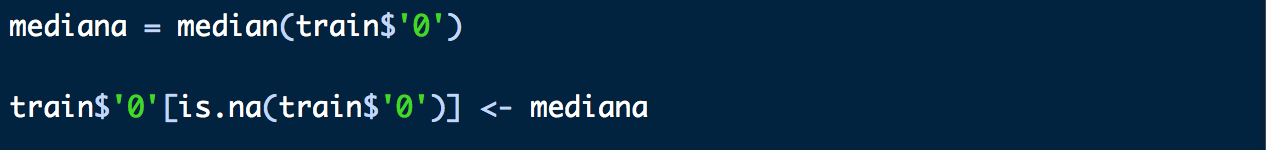
\includegraphics{images/dat15.png}
\caption{\label{fig:"R2"}}
\end{figure}

\begin{itemize}
\tightlist
\item
  Sustitución por la moda: La sustitución por la moda es especialmente útil cuando estamos en presencia de datos categóricos, recordemos que la moda no es mas que el dato que más se repite en el conjunto de datos. Para realizar el cambio usamos \emph{mode()}
\end{itemize}

\begin{figure}
\centering
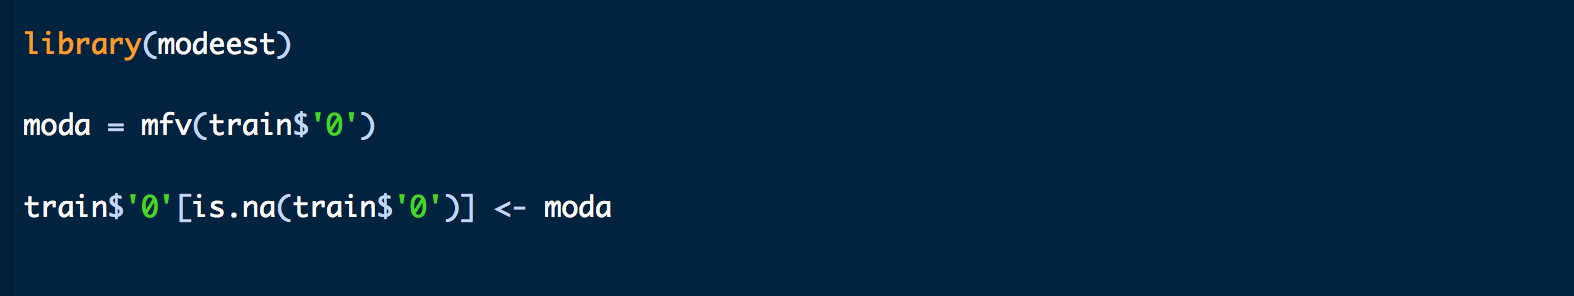
\includegraphics{images/dat16.png}
\caption{\label{fig:"R2"}}
\end{figure}

\begin{enumerate}
\def\labelenumi{(\roman{enumi})}
\setcounter{enumi}{1}
\tightlist
\item
  Missing values en \emph{Python}: Para identificar valores en Python a través de la librería Pandas existen diversas funciones que nos ayudarán. Lo primero que debemos hacer es contar la cantidad de datos faltantes, esto lo hacemos con las funciones \emph{isnull()} y \emph{sum()} de la librería Pandas. El resultado final será el número de missing values por columnas, la primera función los identifica y la segunda función los cuenta. La siguiente imagen muestra cómo hacerlo.
\end{enumerate}

\begin{figure}
\centering
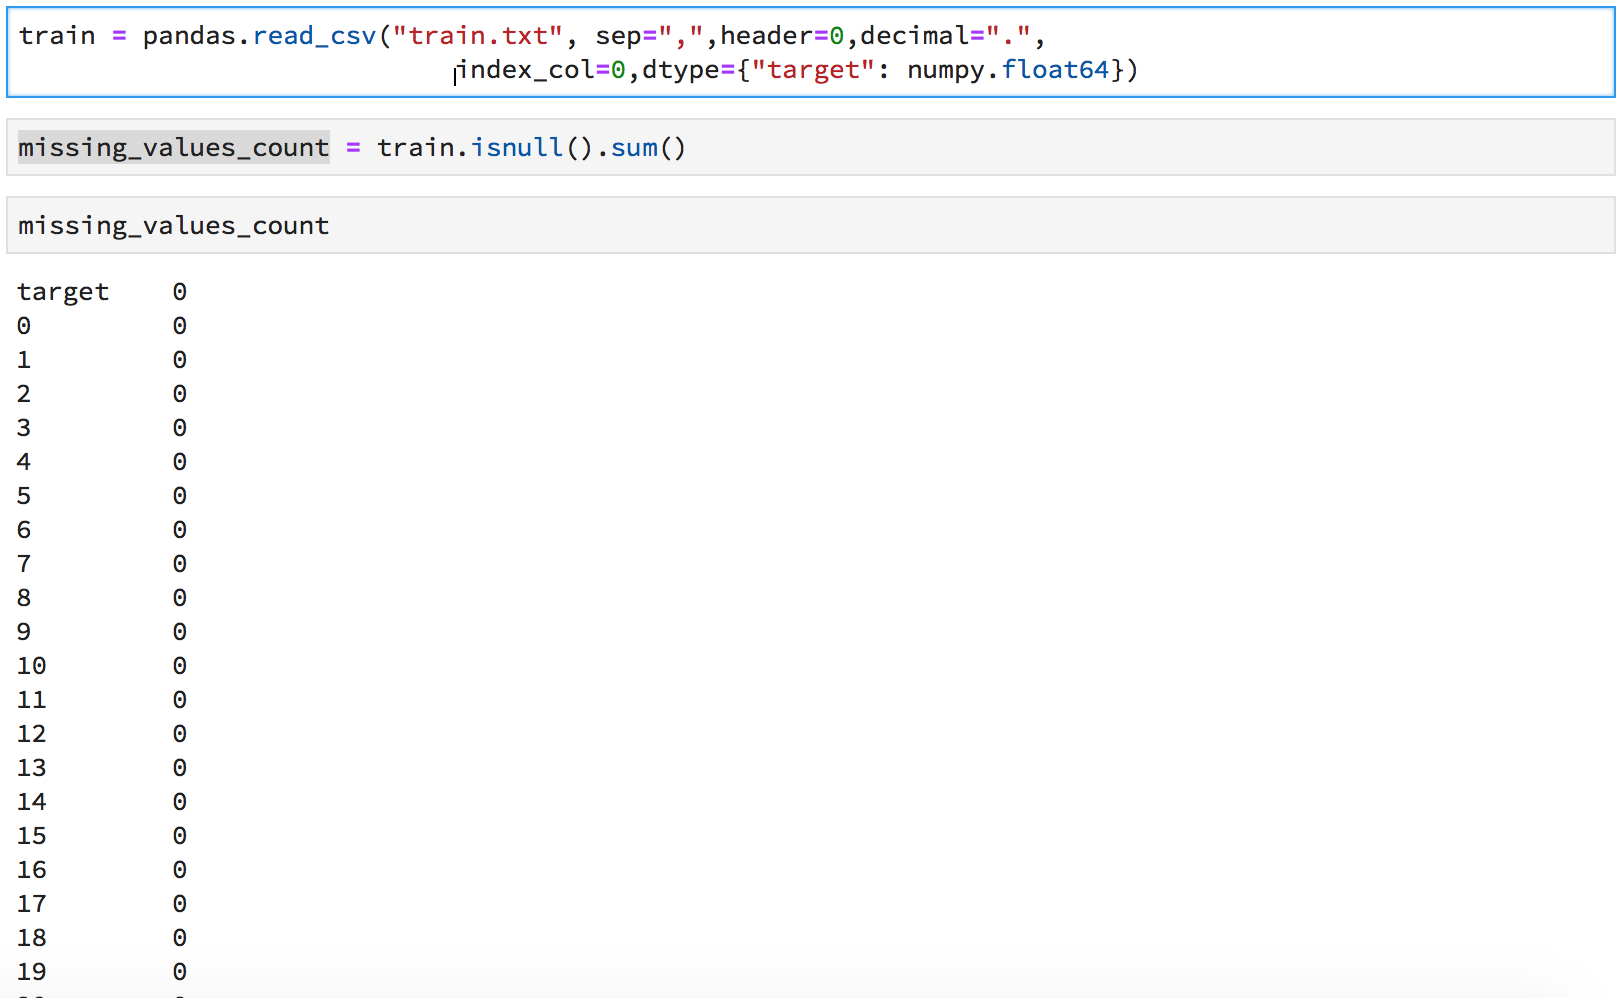
\includegraphics{images/dat6.png}
\caption{\label{fig:"R2"}}
\end{figure}

Ahora si decidimos eliminar los datos, realizar esto en \emph{Python} es sencillo. Primero calculamos el porcentaje de datos faltantes usando las funciones \emph{pandas.shape()}, \emph{pandas.product()}. La primera nos indica la dimensión del dataframe y la segunda realiza la multiplicación para poder saber la cantidad de celdas existentes.

\begin{figure}
\centering
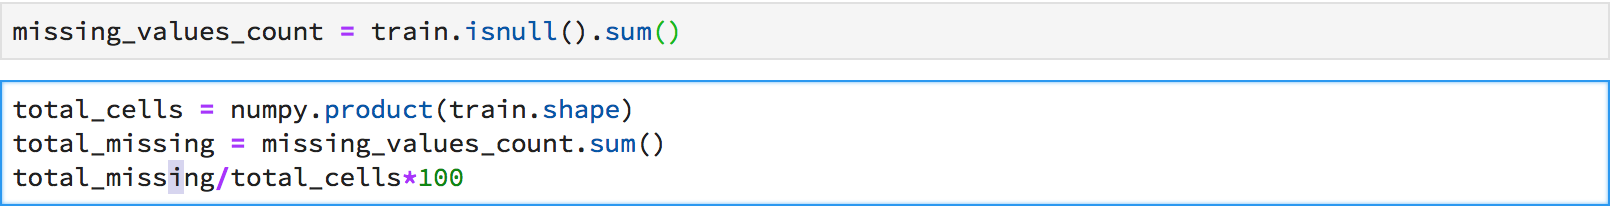
\includegraphics{images/dat7.png}
\caption{\label{fig:"R2"}}
\end{figure}

Luego, dependiendo como estén organizados los datos, es decir, registros por columnas o por filas, sabremos como eliminar los registros con valores faltantes. En la función \emph{df.dropna()}, si colocamos como parámetros \emph{axis=0} se eliminarán los registros por fila que contengan valores faltantes y \emph{axis=1} por columnas.

\begin{figure}
\centering
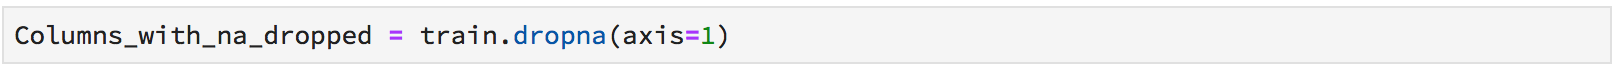
\includegraphics{images/dat8.png}
\caption{\label{fig:"R2"}}
\end{figure}

La otra alternativa con los datos faltantes es imputarlos. Para ello seguiremos el mismo procedimiento usado con \emph{R}, es decir imputación por la media, mediana y moda.

\begin{itemize}
\tightlist
\item
  Sustitución por la media: Para sustituir por el valor medio la función \emph{.mean()} para calcular el valor medio de la columna y la función \emph{.replace()} para realizar el cambio.
\end{itemize}

\begin{figure}
\centering
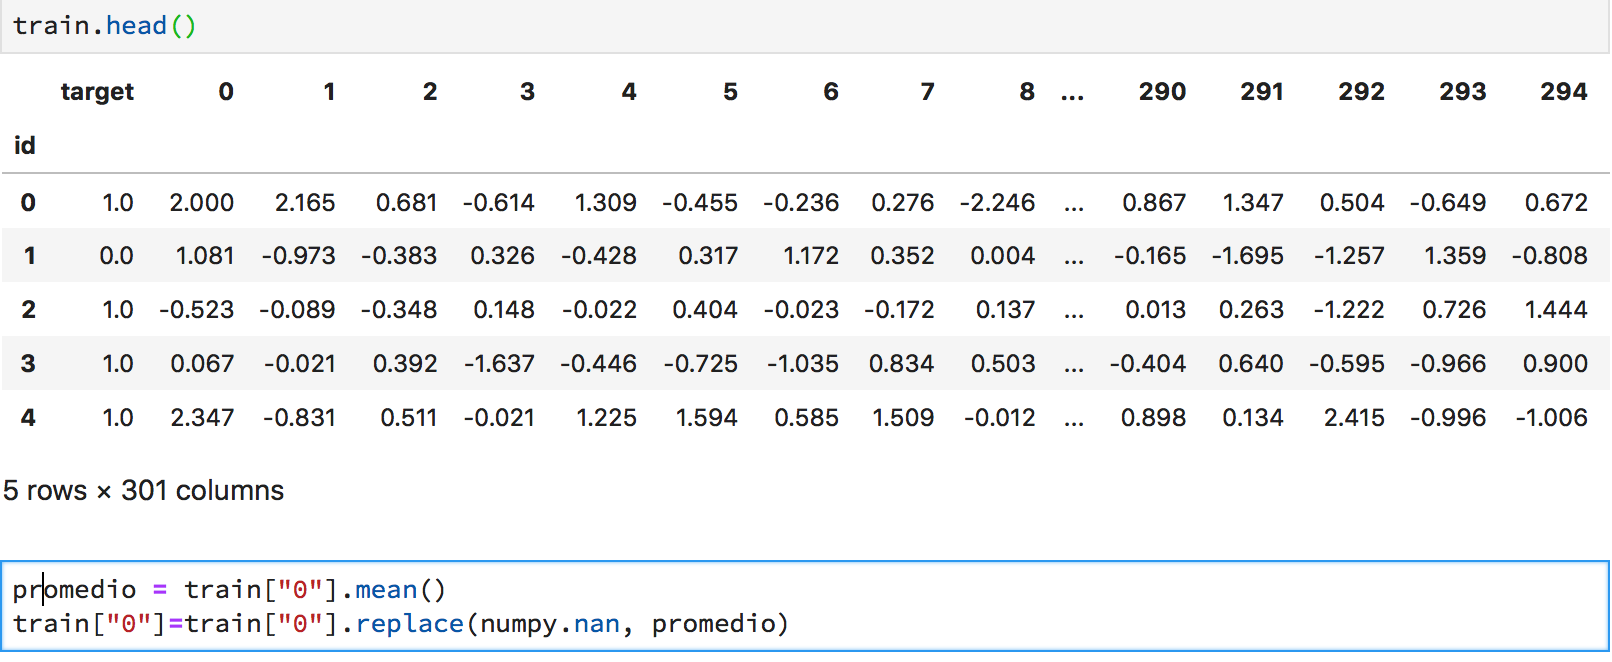
\includegraphics{images/dat11.png}
\caption{\label{fig:"R2"}}
\end{figure}

\begin{itemize}
\tightlist
\item
  Sustitución por la mediana: Para realizar el cambio usamos \emph{.median()}
\end{itemize}

\begin{figure}
\centering
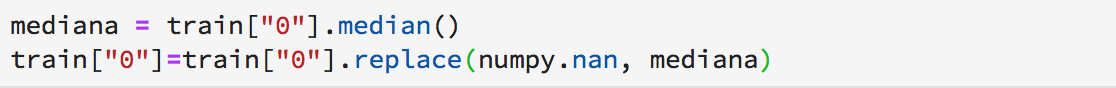
\includegraphics{images/dat12.png}
\caption{\label{fig:"R2"}}
\end{figure}

\begin{itemize}
\tightlist
\item
  Sustitución por la moda: Para realizar el cambio usamos \emph{.mode()}
\end{itemize}

\begin{figure}
\centering
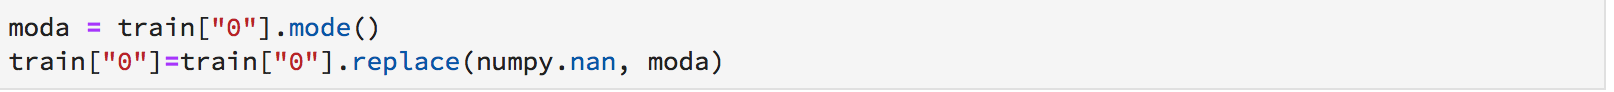
\includegraphics{images/dat13.png}
\caption{\label{fig:"R2"}}
\end{figure}

\hypertarget{identificacion-y-tratamientos-de-outliers-o-puntos-atipicos}{%
\section{Identificación y tratamientos de Outliers o puntos atípicos}\label{identificacion-y-tratamientos-de-outliers-o-puntos-atipicos}}

Los puntos u observaciones atípicas como su nombre lo indica son observaciones que tienen un comportamiento distinto al de las demas observaciones, por ejemplo en el conjunto de datos 2, 3, 2, 4, 3, 2, 34, 3, 2, 1, 2 el valor 34 es un punto atípico. Existen varias razones fundamentales para lo cual es vital detectar estas observaciones entre las que podemos mencionar estan:

\begin{itemize}
\item
  Detectar errores en los datos: Si estamos observando un conjunto de datos donde en una colummna denotamos la edad de los individuos y un individuo tiene en esa entrada -5 o 335 claramente existe un error en los datos
\item
  Encontrar un subconjunto distinto dentro del conjunto original: En algunos casos los valores atípicos señalan la existencias de individuos en particular, cuya existencia puede ser importantes en nuestros estudios.
\item
  Para evitar estimaciones incorrectas en algunos modelos estadísticos: Algunos modelos estadisticos tienen fuertes restricciones en las hipotesis, es por esto que la eliminacion de algunos puntos atípicos puede mejorar de manera significativa nuestros resultados.
\end{itemize}

\hypertarget{identificacion-de-puntos-atipicos}{%
\subsection{Identificación de puntos atípicos}\label{identificacion-de-puntos-atipicos}}

Estudiaremos los dos enfoques más populares: el visual y el cuantitativo

\begin{itemize}
\tightlist
\item
  Visual: Como su nombre lo indica consiste en analizar los datos de manera visual para identificar los valores atípicos. Por ejemplo, en la siguiente imagen podremos notar claramente un par de valores atípicos:
\end{itemize}

\begin{figure}
\centering
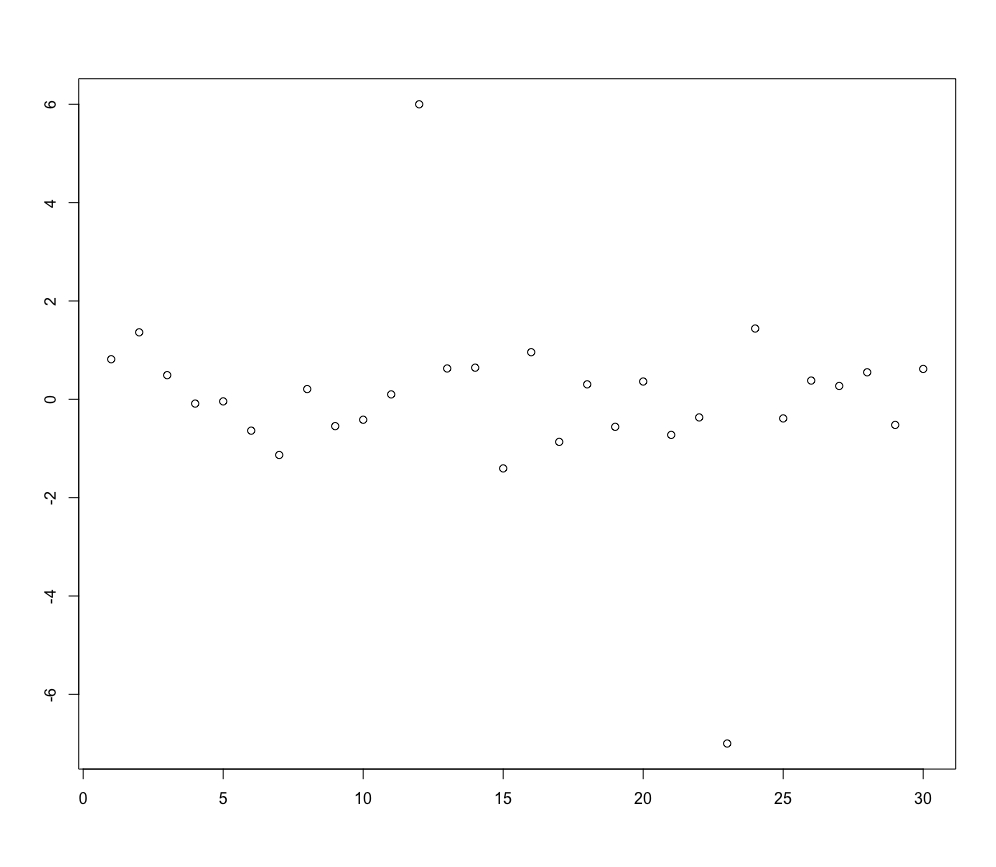
\includegraphics{images/out.png}
\caption{\label{fig:"R2"}}
\end{figure}

El problema se complica cuando aumenta la dimensionalidad del conjunto de datos, es decir, aumentan las categorías que poseen las observaciones. Por ejemplo, supongamos que tenemos un conjunto de datos con tres categorías \(x_1\), \(x_2\), \(x_3\), \(x_4\), en este caso lo usual es graficar el cruce de las variables para encontrar valores atípicos. El problema es que algunos cruces pueden no mostrar nada anormal, como es el cruce entre las variables \(x_1\) y \(x_2\).

\begin{figure}
\centering
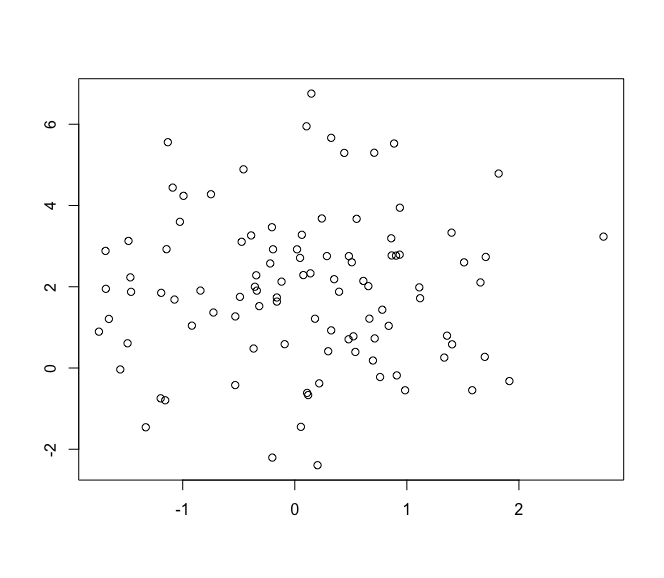
\includegraphics{images/out2.png}
\caption{\label{fig:"R2"}}
\end{figure}

Pero al observar el cruce ente las variables \(x_1\) y \(x_3\) se puede detectar rápidamente el punto atípico.

\begin{figure}
\centering
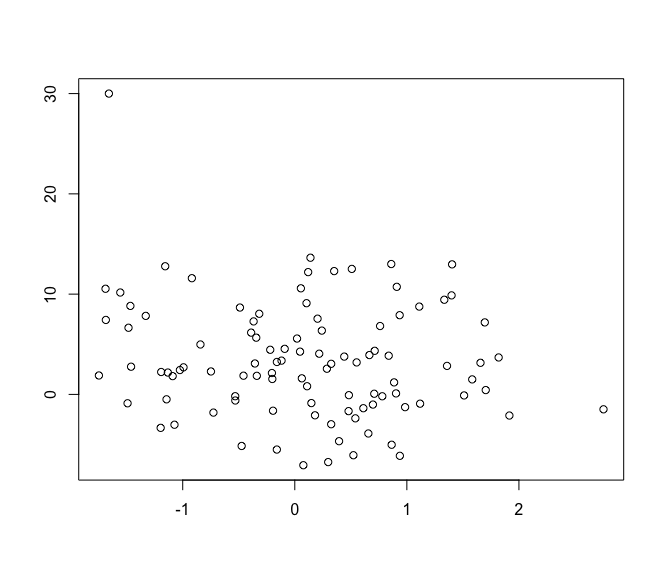
\includegraphics{images/out3.png}
\caption{\label{fig:"R2"}}
\end{figure}

Ahora, es claro que este método puede ser muy ineficiente a la hora de trabajar con una gran cantidad de atributos, es por eso que existe la necesidad de usar algún método cuantitativo para medir si un dato es atípico o no. Uno de los más utilizado es el método basado en la medida o distancia \(D_M\) de \emph{Mahalanobis}

\begin{itemize}
\tightlist
\item
  \(D_M\) de \emph{Mahalanobis}: Es una medida de distancia introducida por \emph{Prasanta Chandra Mahalanobis} y su principal uso era determinar la similitud entre dos variables aleatorias. Su gran característica es que usa la matriz de covarianza para dar un peso ponderado por esta matriz a cada variable. Su gran desventaja es que es sensible a las escalas de los datos, por lo que se sugiere escalar los datos ya sea por su media u otro criterio similar.
\end{itemize}

En general, debemos tener un punto de referencia para poder medir la proximidad de los puntos que estamos midiendo, lo común es usar la media o la mediana, la ecuación que representa la distancia \(D_M\) de \emph{Mahalanobis} es:

\[\sqrt{(x-y)^{T} \Sigma^{-1}(x-y)}\]

Donde \(y\) es el punto fijo de referencia, \(x\) es el punto al que le estamos calculando la distancia y \(\Sigma\) la matriz de covarianza.

\hypertarget{deteccion-de-outliers-en-r}{%
\subsection{Detección de outliers en R}\label{deteccion-de-outliers-en-r}}

\begin{itemize}
\tightlist
\item
  Visual: Supongamos que tenemos el conjunto Data previamente cargado y compuesto por tres variables \(x_1\), \(x_2\) y \(x_3\). Usaremos la función \(plot()\), para observar la variable \(x_1\). Usamos el siguiente comando:
\end{itemize}

\begin{figure}
\centering
\includegraphics{images/out5.png}
\caption{\label{fig:"R2"}}
\end{figure}

Dando como resultado:

\begin{figure}
\centering
\includegraphics{images/out4.png}
\caption{\label{fig:"R2"}}
\end{figure}

A primera vista no hay ningún valor atípico, sin embargo, si generamos el mismo gráfico para la variable \(x_3\), obtenemos claramente un outlier:

\begin{figure}
\centering
\includegraphics{images/out6.png}
\caption{\label{fig:"R2"}}
\end{figure}

Ahora si queremos hacer el cruce de variables, usamos igual el mismo comando, por ejemplo, el de las variables \(x_1\) y \(x_2\), hacemos:

\begin{figure}
\centering
\includegraphics{images/out7.png}
\caption{\label{fig:"R2"}}
\end{figure}

Aparentemente no se observan outliers, como muestra la siguiente imagen.

\begin{figure}
\centering
\includegraphics{images/out8.png}
\caption{\label{fig:"R2"}}
\end{figure}

Ahora, si realizamos el cruce de las variables \(x_1\) y \(x_3\) obtenemos:

\begin{figure}
\centering
\includegraphics{images/out9.png}
\caption{\label{fig:"R2"}}
\end{figure}

Observando claramente un outlier, que posee un valor de 30. Ahora si tenemos muchas variables, este proceso se complica, es por esto que usaremos la distancia \(D_M\) de \emph{Mahalanobis}.

\begin{itemize}
\tightlist
\item
  la distancia \(D_M\) de \emph{Mahalanobis}: Para calcular la distancia de Mahalanobis debemos calcular primero el punto de referencia, en nuestro caso la media, usaremos la función \emph{apply()}, la función \emph{cov()} para calcular la matriz de covarianza y al final usamos la función \emph{mahalanobis()} indicándole los datos a calcular. Luego usamos la función \emph{plot()} para ver la existencia de valores atípicos.
\end{itemize}

\begin{figure}
\centering
\includegraphics{images/out10.png}
\caption{\label{fig:"R2"}}
\end{figure}

\begin{figure}
\centering
\includegraphics{images/out11.png}
\caption{\label{fig:"R2"}}
\end{figure}

\hypertarget{deteccion-de-outliers-en-python}{%
\subsection{Detección de outliers en Python}\label{deteccion-de-outliers-en-python}}

\begin{itemize}
\tightlist
\item
  Visual: Para identificar outliers de manera visual en \emph{Python} haremos uso de la librería \emph{Matplotlib}, la cual nos brinda un sinfín de herramientas para poder llevar a cabo nuestros objetivos. Al igual que en la sección anterior usaremos el conjunto de datos Data con tres variables.
\end{itemize}

Para ver la gráfica de la variable \(x_1\), primero debemos seleccionar la variable, esto lo hacemos con el método \emph{.iloc()} de \emph{Pandas} el cual nos permite seleccionar subconjuntos de datos. Luego, usamos \emph{plt.plot()} para generar la gráfica de los datos, el parámetro ro indica el tipo de gráfico, en nuestro caso en punteado; \emph{plt.xlabel} para dar título al eje horizontal y \emph{plt.ylabel} para dar título al eje vertical, finalmente usamos \emph{plt.show} para mostrar la imagen.

Al graficar la variable \(x_1\), se observa que carece de valores atípicos:

\begin{figure}
\centering
\includegraphics{images/out14.png}
\caption{\label{fig:"R2"}}
\end{figure}

\begin{figure}
\centering
\includegraphics{images/out16.png}
\caption{\label{fig:"R2"}}
\end{figure}

Pero cuando generamos el gráfico de la variable \(x_3\) notamos el valor atípico:

\begin{figure}
\centering
\includegraphics{images/out15.png}
\caption{\label{fig:"R2"}}
\end{figure}

Para realizar el gráfico del cruce de variables, simplemente agregamos la variable adicional como parámetro en \emph{plt.plot()}.En este caso tampoco se observan valores atípicos.

\begin{figure}
\centering
\includegraphics{images/out17.png}
\caption{\label{fig:"R2"}}
\end{figure}

Pero al realizar el cruce con las variables \(x_1\) y \(x_3\) notamos el valor atípico.

\begin{figure}
\centering
\includegraphics{images/out18.png}
\caption{\label{fig:"R2"}}
\end{figure}

\begin{itemize}
\tightlist
\item
  La distancia \(D_M\) de \emph{Mahalanobis}: Para calcular la distancia de \emph{Mahalanobis} de un conjunto de datos usando \emph{Python}, usaremos la librería \emph{Scipy} la cual trae por defecto una función para calcular la distancia de Mahalanobis. Primero debemos calcular la media de las columnas, usando la función \emph{.mean()} de \emph{Pandas}. A diferencia de \emph{R}, debemos calcular la inversa de la matriz de covarianza (\emph{Python} trae por defecto las filas y columnas intercambiadas con respecto a \emph{R}), para ello usamos la funciones \emph{.cov()}, la cual calcula la matriz de covarianza, \emph{.linalg()} y \emph{.inv()} para calcular la inversa. Luego, usando la función \emph{apply()} de \emph{Pandas} para aplicar la función \emph{mahalanobis()} de la libreria \emph{Scipy} a todo el conjunto de datos. En la función \emph{.apply()} debemos colocar el nombre de la función, \emph{axis} para indicar si la función aplica a las columnas o filas: el valor de \(0\) para las columnas y \(1\) para las filas. Finalizamos con \emph{args} que contiene los parámetros que necesita la función, en nuestro caso el punto de referencia, el cual es la media por columnas y la inversa de la matriz de covarianza.
\end{itemize}

\begin{figure}
\centering
\includegraphics{images/out21.png}
\caption{\label{fig:"R2"}}
\end{figure}

Podremos notar claramente un valor atípico en la siguiente imagen.

\begin{figure}
\centering
\includegraphics{images/out20.png}
\caption{\label{fig:"R2"}}
\end{figure}

\hypertarget{regresion-lineal}{%
\chapter{Regresión Lineal}\label{regresion-lineal}}

La regresión lineal es un método estadístico que intenta predecir una variable de interés (dependiente) a partir de otras variables que se consideran influyentes (independientes) y se relacionan directamente con ella. Por ejemplo, hay estudios que sugieren la relacion entre el tamaño del pétalo (\(P\)) y el sépalo de una flor (\(S\)), en algunal flores se aproxima el tamaño del pétalo multiplicando por 3 el tamaño del sépalo, es decir, \(P=3*S\), esta relación es un ejemplo simple de lo que es la regresión lineal de solo dos variables.

En general si tenemos una variable \(y\) dependiente y \(n\) variables independientes \(x_1, x_2, ..., x_n\) un modelo de regresión lineal tiene la forma \[y=c+c_1x_1+c_2x_2+...+c_nx_n\] donde los coeficientes \(c_j\) son los coeficientes del modelo y \(c\) es el coeficiente independiente, en algunos casos es llamado intercept.

\hypertarget{identificando-relacion-entre-variables}{%
\section{Identificando relación entre variables}\label{identificando-relacion-entre-variables}}

Una de las primeras cosas a verificar antes de realizar el análisis de regresión es comprobar la relación existente entre la variable dependiente con las variables independientes, para lo cual existen diversas maneras de hacerlo:

\begin{itemize}
\tightlist
\item
  Visual: Se realiza un gráfico entre la variable dependiente y la variable independiente a estudiar, si se nota un tipo de linealidad entre los datos podemos pensar en incluir la variable independiente en el modelo. Por ejemplo, en el siguiente ejemplo se nota una cierta linealidad entre las variables.
\end{itemize}

\begin{figure}
\centering
\includegraphics{images/reg.png}
\caption{\label{fig:"R2"}}
\end{figure}

\begin{itemize}
\tightlist
\item
  Cuantitativa: Una manera cuantitativa de medir la relación entre variables es usar el índice de correlacion, el cual varía entre -1 y 1. Entre más cerca de -1 o 1 esté el índice de correlación entre variables, mayor es su relación, en general, decimos que existe correlación lineal entre las variables independientes si el índice de correlación entre las variables es mayor a 0.5 o menor a -0.5.
\end{itemize}

Usaremos el conjunto de datos \emph{mtcars} en \emph{R} para ilustrar de ahora en adelante el proceso de regresión lineal. Los datos fueron extraídos de la revista Motor Trend US de 1974, y comprenden el consumo de combustible y 10 aspectos del diseño y rendimiento de los automóviles para 32 automóviles (modelos 1973-74).

\hypertarget{identificando-relacion-entre-variables-con-r}{%
\subsection{\texorpdfstring{Identificando relación entre variables con \emph{R}}{Identificando relación entre variables con R}}\label{identificando-relacion-entre-variables-con-r}}

\begin{itemize}
\tightlist
\item
  Visual: Usamos la función \emph{plot()} vista previamente para graficar el cruce entre variables, por ejemplo, entre las variables \emph{mpg} (Millas/(US) por galón) y \emph{disp} (Desplazamiento) notamos un cierto comportamiento lineal.
\end{itemize}

\begin{figure}
\centering
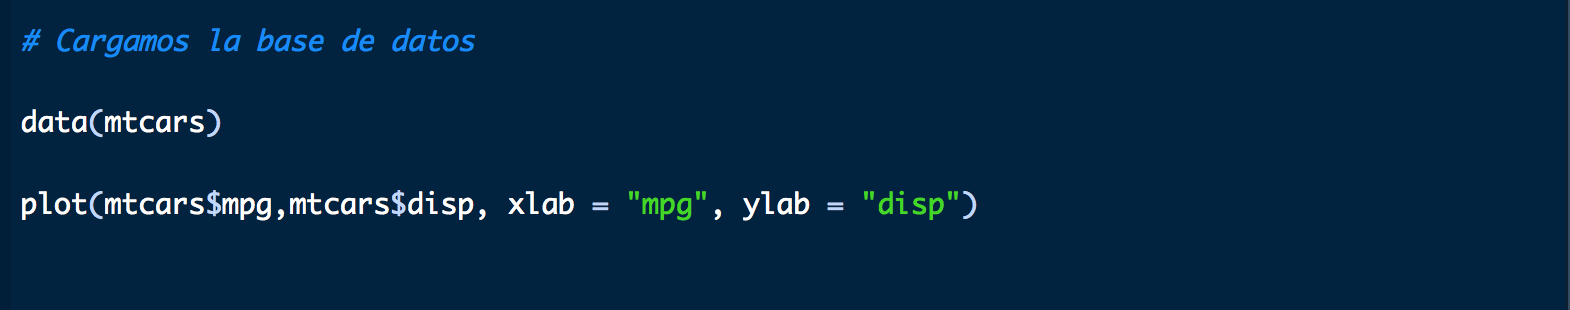
\includegraphics{images/reg3.png}
\caption{\label{fig:"R2"}}
\end{figure}

\begin{figure}
\centering
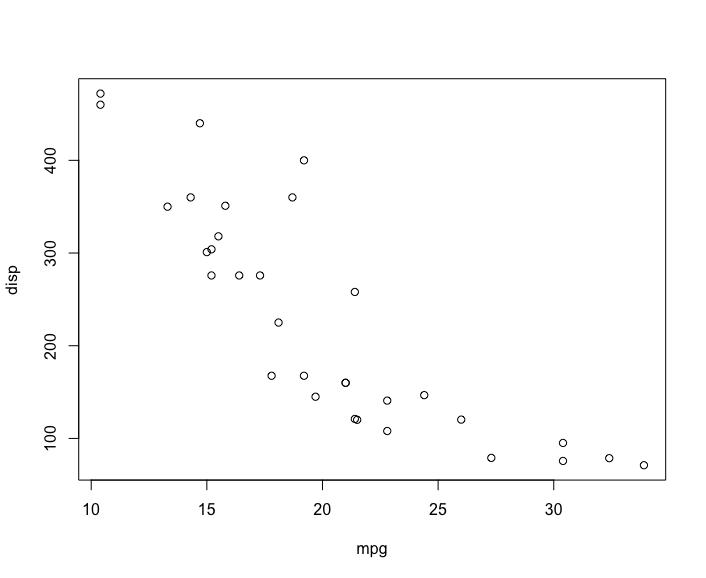
\includegraphics{images/reg2.png}
\caption{\label{fig:"R2"}}
\end{figure}

Con la función \emph{plot()} tenemos la ventaja de que simplemente pasando como argumento el conjunto de datos arroja una imagen con todos los cruces posibles entre las once (11) variables de la base de datos mtcars.

\begin{figure}
\centering

\includegraphics{images/reg5.png}
\caption{\label{fig:"R2"}}
\end{figure}

\begin{figure}
\centering
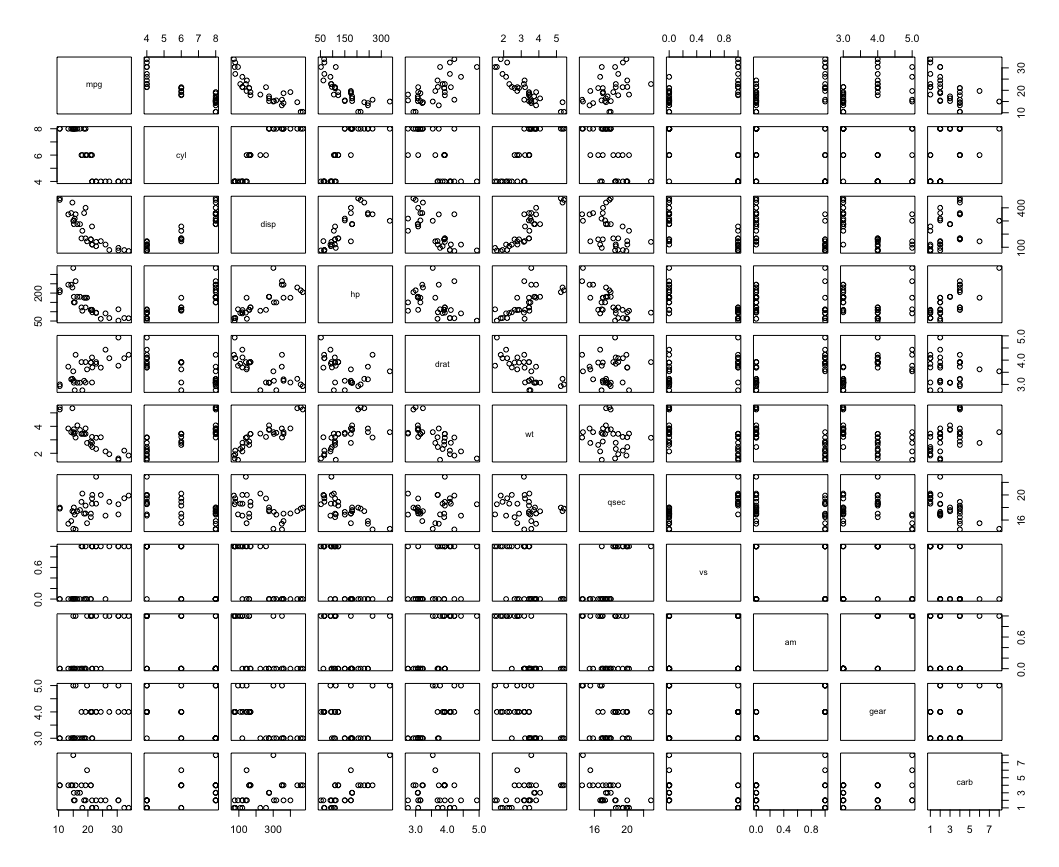
\includegraphics{images/reg4.png}
\caption{\label{fig:"R2"}}
\end{figure}

\begin{itemize}
\tightlist
\item
  Cuantitativa: La función \emph{cor()} permite hallar la correlación entre las variables, por ejemplo entre \emph{mpg} y \emph{disp}
\end{itemize}


\includegraphics{images/reg6.png}
Este valor -0.84 nos confirma la posible relación que existe entre las variables \emph{mpg} y \emph{disp}. De igual manera podemos aplicar la función \emph{cor()} a todo el conjunto de datos arrojando una matriz con todo los valores posibles de correlaciones.

\begin{figure}
\centering
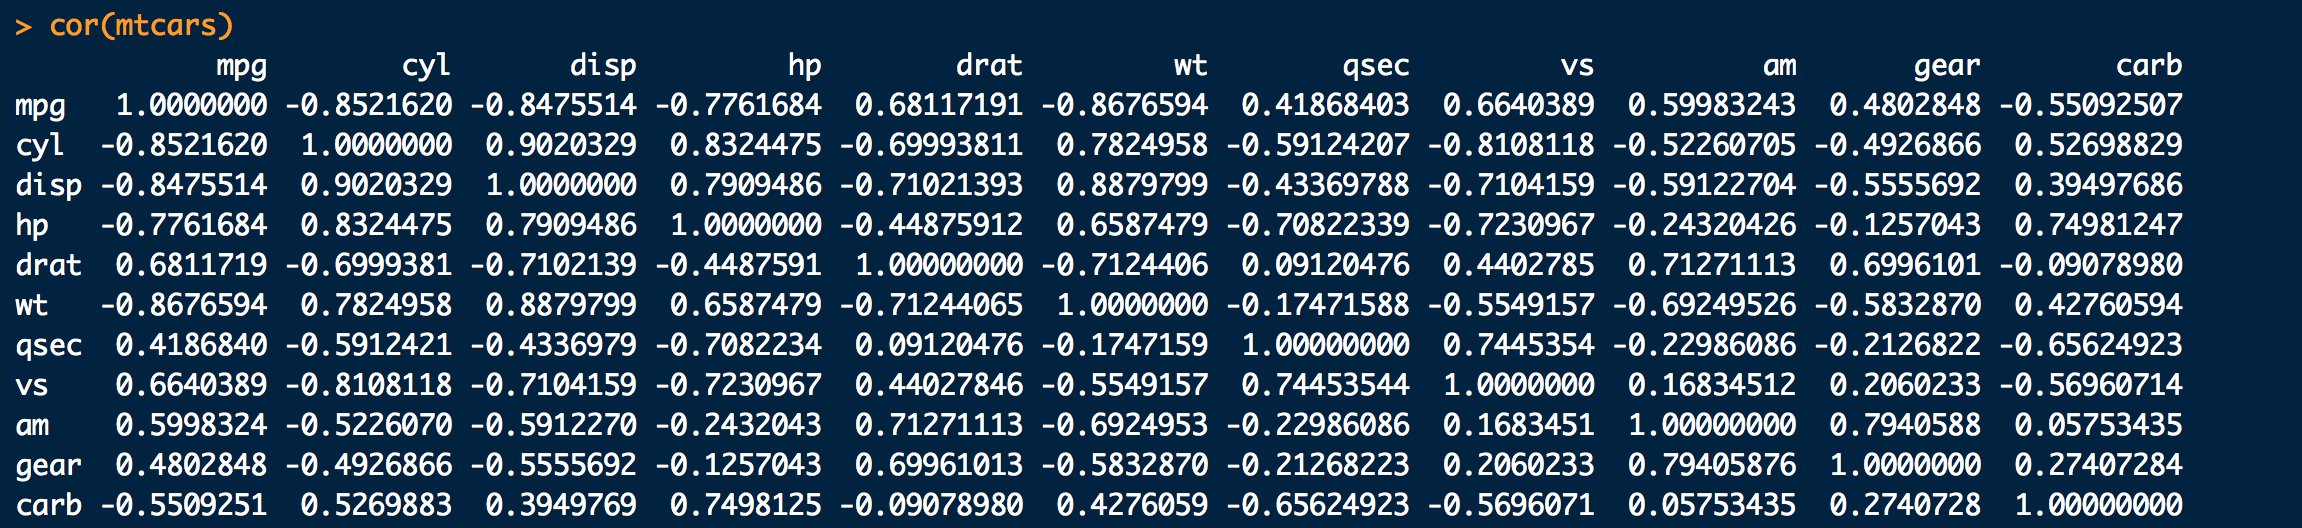
\includegraphics{images/reg7.png}
\caption{\label{fig:"R2"}}
\end{figure}

\hypertarget{identificando-relacion-entre-variables-con-python}{%
\subsection{\texorpdfstring{Identificando relación entre variables con \emph{Python}}{Identificando relación entre variables con Python}}\label{identificando-relacion-entre-variables-con-python}}

\begin{itemize}
\tightlist
\item
  Visual: En Python usaremos de nuevo la librería \emph{Matplotlib}, para obtener el gráfico del cruce entre variables, de igual manera notaremos el comportamiento lineal entre las variables.
\end{itemize}

\begin{figure}
\centering
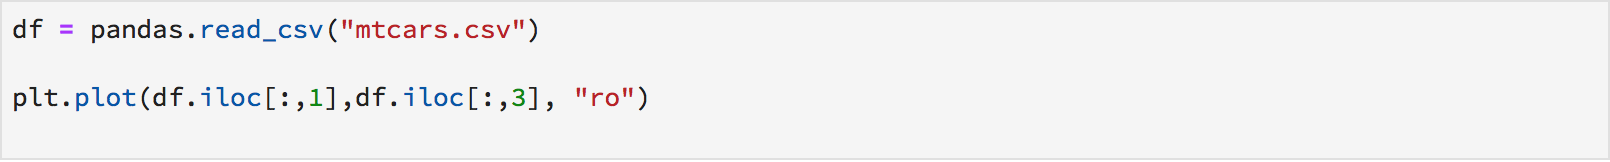
\includegraphics{images/reg9.png}
\caption{\label{fig:"R2"}}
\end{figure}

\begin{figure}
\centering
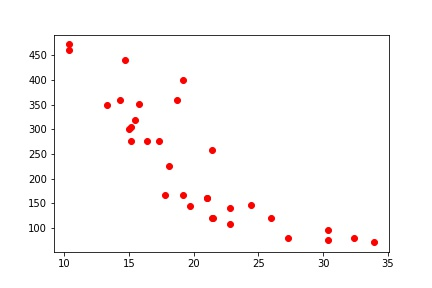
\includegraphics{images/reg8.jpg}
\caption{\label{fig:"R2"}}
\end{figure}

Ahora, si queremos realizar un solo gráfico con el cruce de todas las variables, como el caso de la función \emph{cor()} en \emph{R}, debemos implementar una librería llamada \emph{Seaborn}, la cual arrojará el resultado deseado haciendo uso de la función \emph{.pairplot()}, con los argumentos: \emph{kind} (para el tipo de gráfico) y \emph{palette} (para el color).

\begin{figure}
\centering
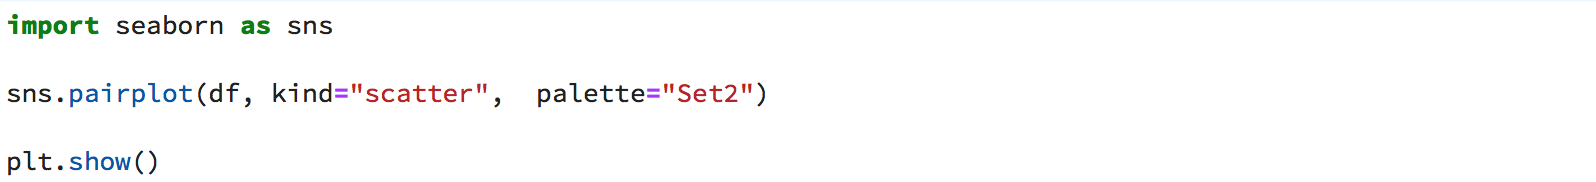
\includegraphics{images/reg11.png}
\caption{\label{fig:"R2"}}
\end{figure}

\begin{figure}
\centering
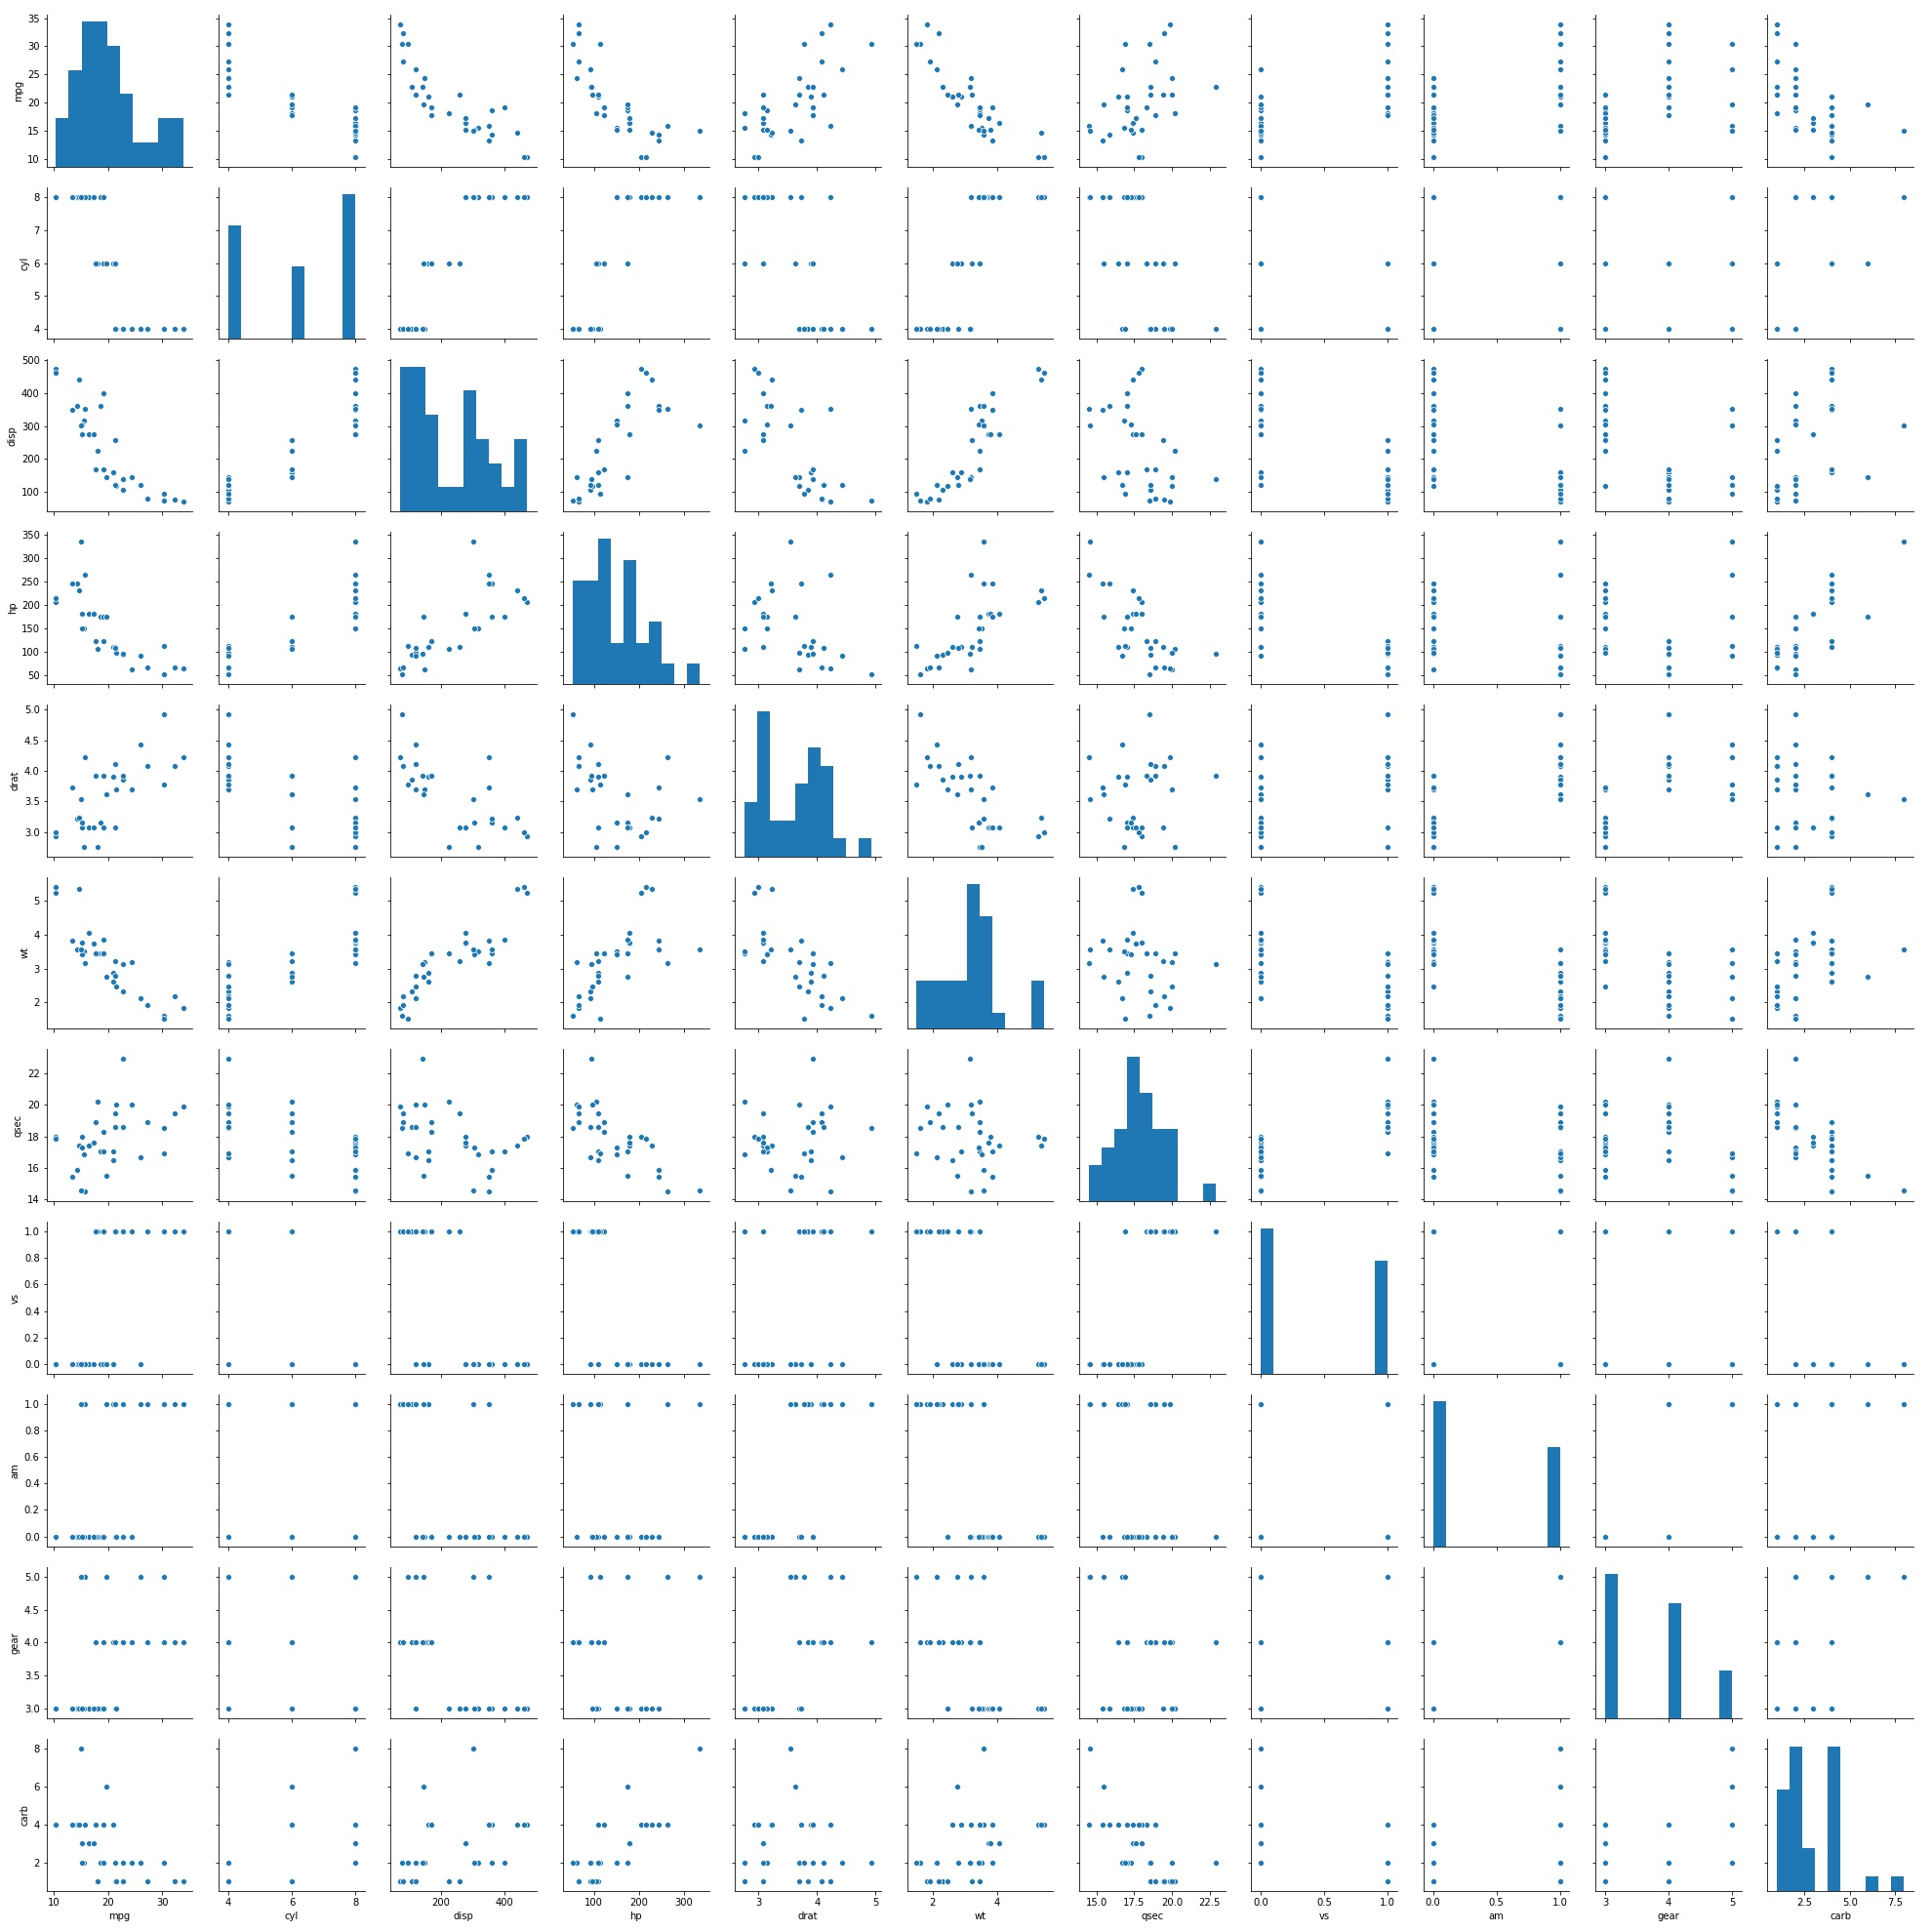
\includegraphics{images/reg10.jpg}
\caption{\label{fig:"R2"}}
\end{figure}

\begin{itemize}
\tightlist
\item
  Cuantitativo: Para obtener la matriz de correlación entre las variables de nuestro conjunto de datos, hacemos uso de la función \emph{.cor()} de la librería \emph{Pandas}. En el caso que queramos alguna correlación en específico filtramos los elementos de la matriz anterior.
\end{itemize}

\begin{figure}
\centering
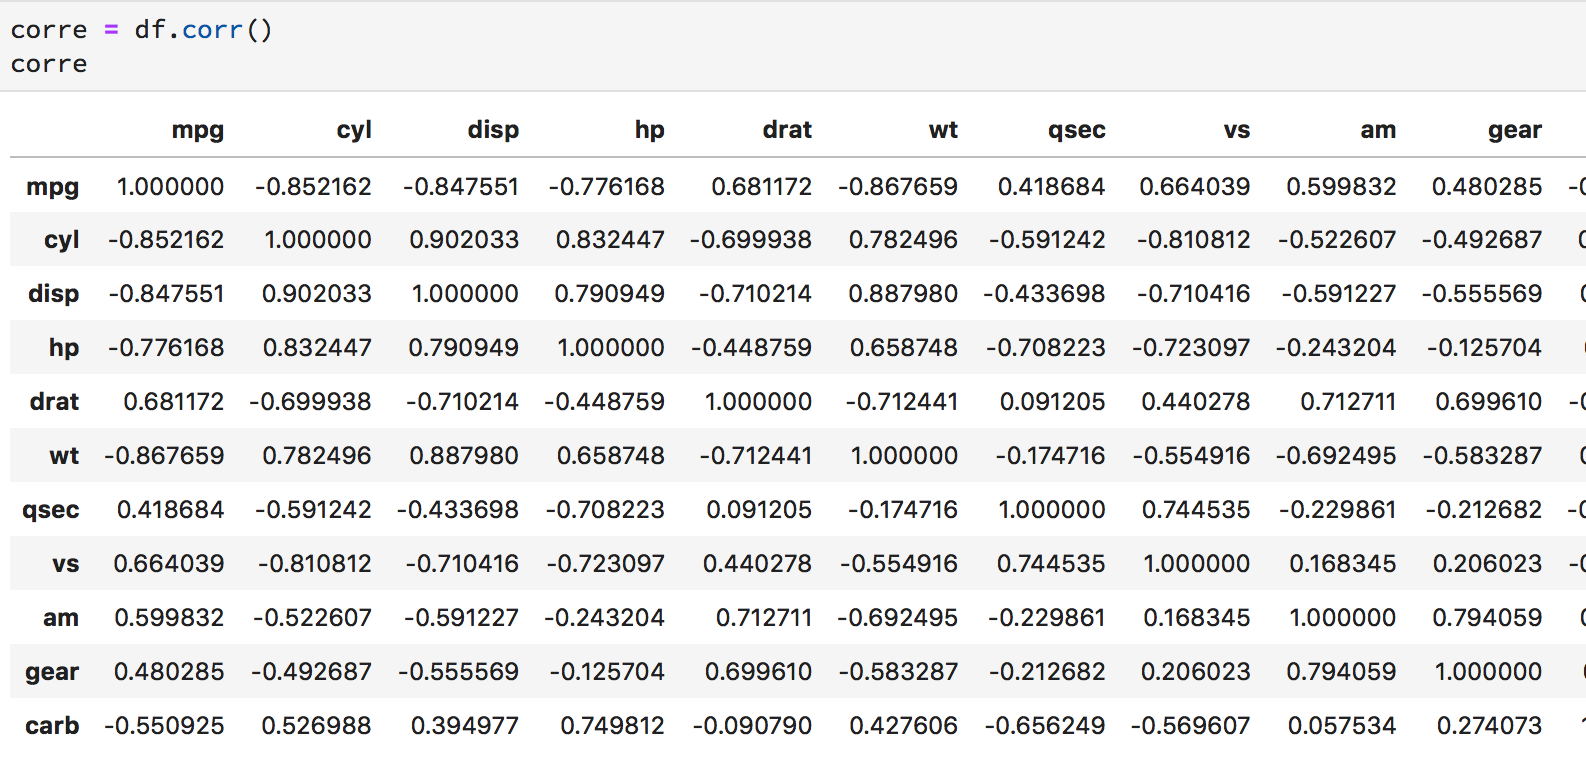
\includegraphics{images/reg12.png}
\caption{\label{fig:"R2"}}
\end{figure}

\hypertarget{transformando-variables}{%
\section{Transformando variables}\label{transformando-variables}}

Una de las principales hipótesis en la regresión lineal es la normalidad de las variables implicadas, es decir, que las variables provengan de una distribución normal. Pero, ¿cómo identificamos este comportamiento en una variable? La forma más sencilla es inspeccionando el histograma proveniente de dicha variable y corroborando si existe un comportamiento acampanado, como en el siguiente ejemplo:

\begin{figure}
\centering
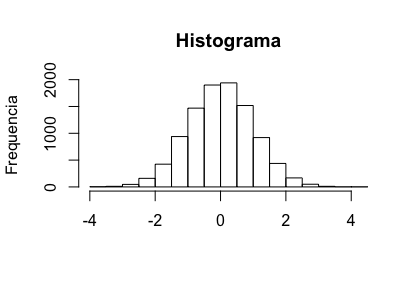
\includegraphics{images/reg13.png}
\caption{\label{fig:"R2"}}
\end{figure}

Pero en muchos casos, las variables no poseen este comportamiento, por lo tanto se debe aplicar transformaciones que imiten el comportamiento acampanado de la gráfica anterior. Las transformaciones más comunes son: \(y=x^2\), \(y=\sqrt{x}\), \(y=ln(x)\) y \(y=\frac{1}{x}\). En las siguientes gráficas podemos apreciar el efecto de estas transformaciones:

\begin{figure}
\centering
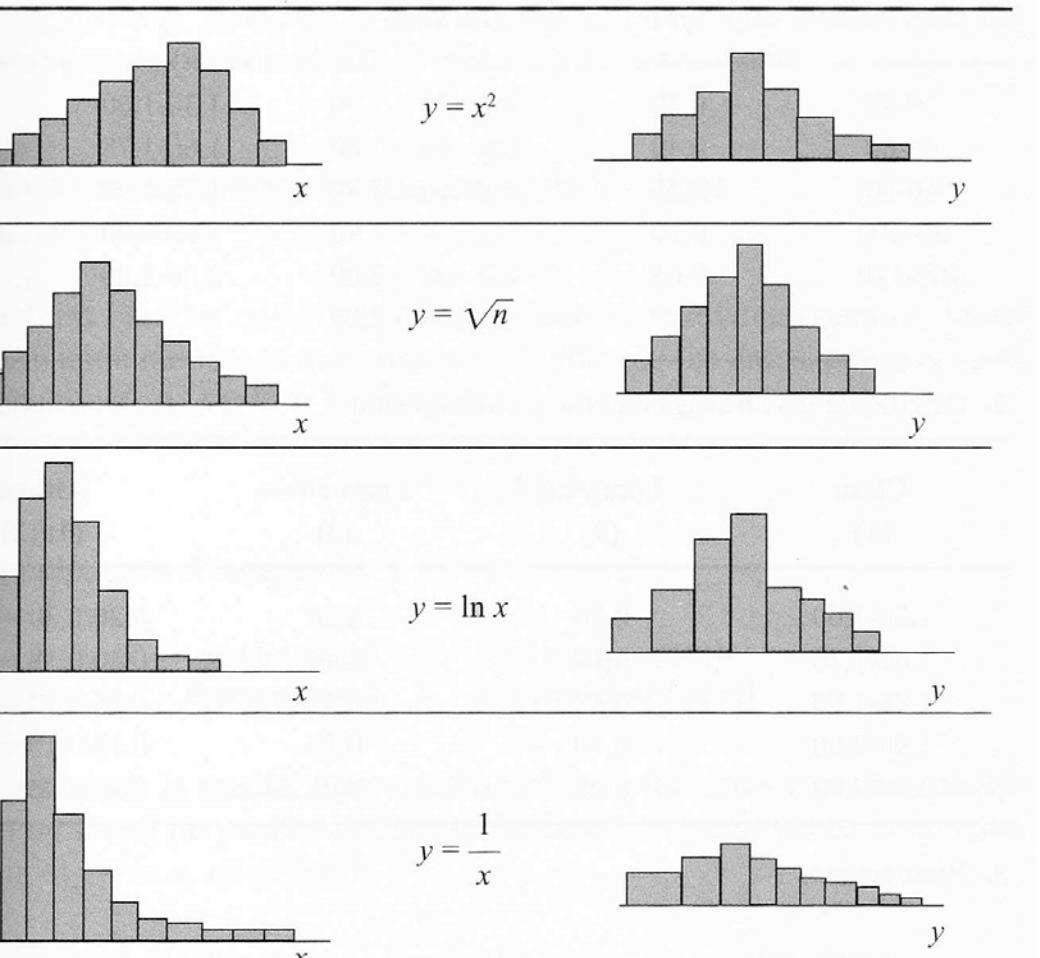
\includegraphics{images/reg14.png}
\caption{\label{fig:"R2"}}
\end{figure}

Esta última imagen nos da una idea de cuando debemos aplicar alguna de las transformaciones anteriores. Ahora veremos cómo aplicarlas en los respectivos lenguajes

\hypertarget{aplicando-transformaciones-de-variables-en-r}{%
\subsection{\texorpdfstring{Aplicando transformaciones de variables en \emph{R}}{Aplicando transformaciones de variables en R}}\label{aplicando-transformaciones-de-variables-en-r}}

Esta tarea es muy fácil de ejecutar en \emph{R}, supongamos que estamos trabajando con la variable \emph{x} del conjunto de datos \emph{df}, los códigos para realizar estas transformaciones son:

\begin{figure}
\centering
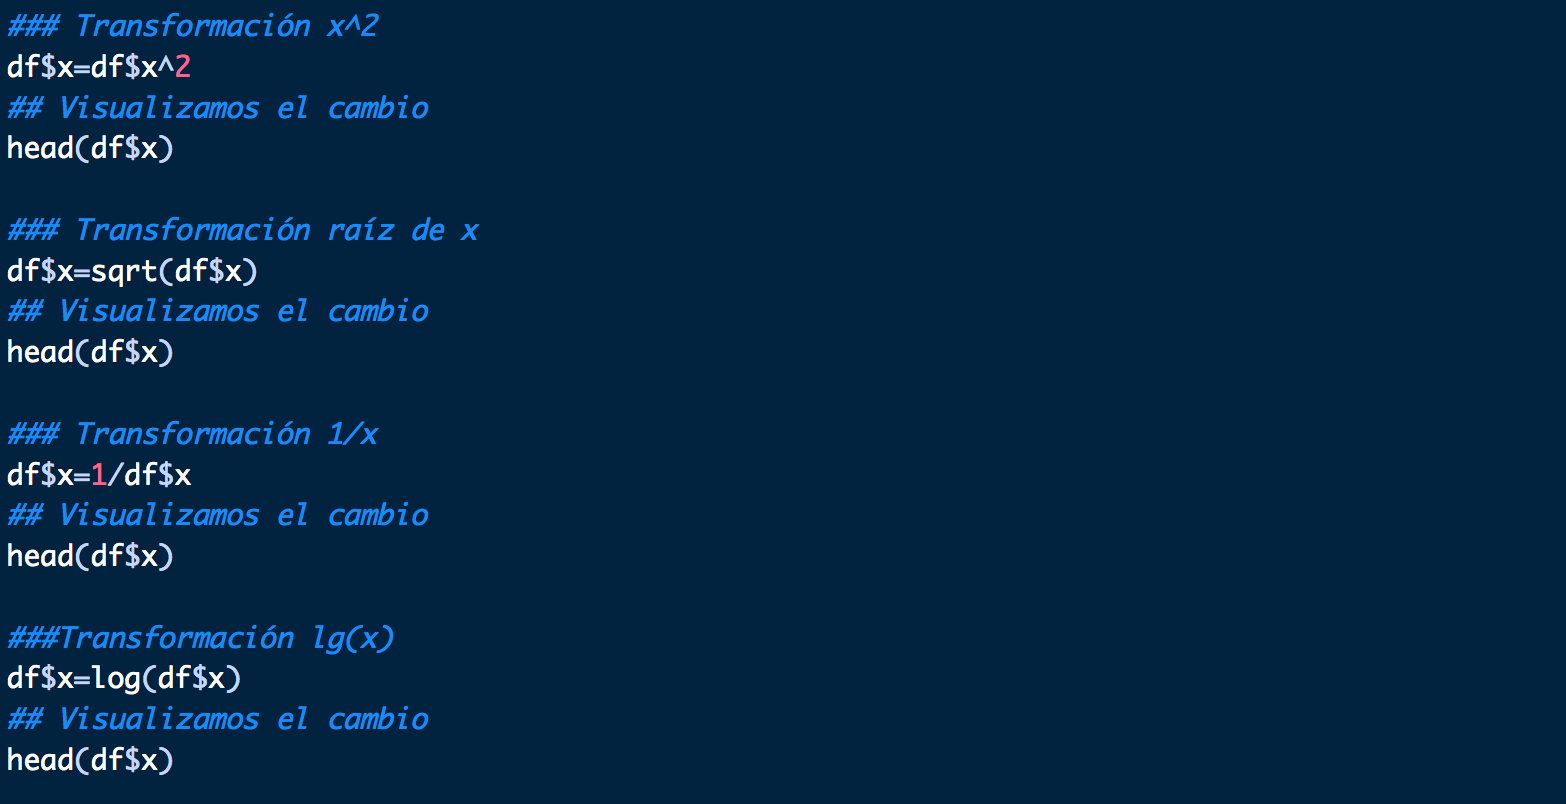
\includegraphics{images/reg15.png}
\caption{\label{fig:"R2"}}
\end{figure}

\hypertarget{aplicando-transformaciones-de-variables-en-python}{%
\subsection{\texorpdfstring{Aplicando transformaciones de variables en \emph{Python}}{Aplicando transformaciones de variables en Python}}\label{aplicando-transformaciones-de-variables-en-python}}

En Python es fácil realizar las transformaciones menos la del logaritmo, para la cual usaremos la librería \emph{Math} en específico la función \emph{.log()} junto a la función \emph{.apply}, pues la función \emph{.log()} se aplica a números y queremos aplicarla a una variable completa.

\begin{figure}
\centering
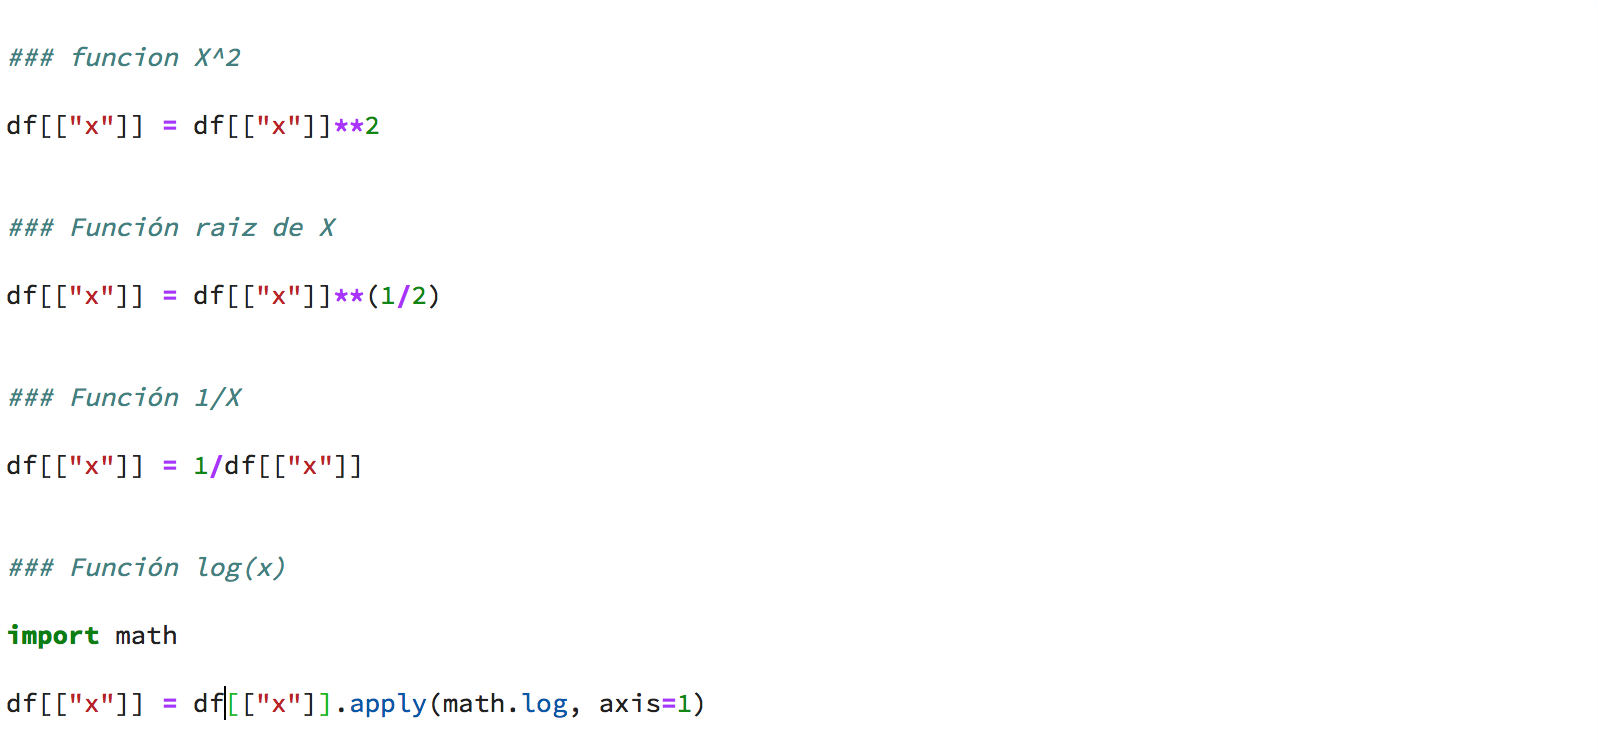
\includegraphics{images/reg16.png}
\caption{\label{fig:"R2"}}
\end{figure}

\hypertarget{eliminando-el-efecto-de-colinealidad-entre-variables-independientes.}{%
\section{Eliminando el efecto de colinealidad entre variables independientes.}\label{eliminando-el-efecto-de-colinealidad-entre-variables-independientes.}}

Otra hipótesis importante antes de realizar el modelo de regresión, es la no colinealidad entre las variables, es decir, inexistencia de una relación lineal entre variables independientes. En caso de descubrir este efecto debemos eliminar una de estas variables y quedarnos con la otra.

La forma de identificar colinealidad es exactamente igual a la forma de encontrar correlaciones entre las variables vistas al principio de este capítulo. Primero calculamos el índice de correlación entre variables, si se encuentra una alta correlación entre un par de variables independientes se procede a revisar la gráfica del cruce de dichas variable, y si se observa una clara relación lineal procedemos a eliminar alguna de ellas.

\hypertarget{eliminacion-de-las-variables-categoricas}{%
\section{Eliminación de las variables categóricas}\label{eliminacion-de-las-variables-categoricas}}

En los modelos de regresión lineal las variables categóricas no cumplen las hipótesis del modelo, pues no satisfacen el supuesto de normalidad. Recordemos que una variable categórica es una variable que toma unos valores fijos ya conocidos, por ejemplo, la variable que toma los valores 1,2,3,4,5,6 que representa los posibles valores que toma el lanzamiento de un dado, es una variable categórica, o la variable que toma los valores de Si o No que se refiere al consumo de un producto específico. Por lo tanto debemos saber cómo eliminar variables de nuestro conjunto de datos.

\hypertarget{eliminacion-de-variables-en-r}{%
\subsection{\texorpdfstring{Eliminación de variables en \emph{R}}{Eliminación de variables en R}}\label{eliminacion-de-variables-en-r}}

Supongamos que tenemos en un conjunto de datos llamados \emph{mtcars} la variable \emph{mpg} la cual deseamos eliminar. Para ello usamos el siguiente código, en el cual el símbolo \emph{!} es el indicador para eliminar dicha variable.

\begin{figure}
\centering

\includegraphics{images/reg17.png}
\caption{\label{fig:"R2"}}
\end{figure}

Para recuperar la columna eliminada se vuelve a cargar la base de datos \emph{data(mtcars)}.

\hypertarget{eliminacion-de-variables-en-python}{%
\subsection{\texorpdfstring{Eliminación de variables en \emph{Python}}{Eliminación de variables en Python}}\label{eliminacion-de-variables-en-python}}

De igual manera suponiendo que tenemos el mismo conjunto de datos y la misma variable a eliminar en \emph{Python}, usamos la función \emph{.drop()} para eliminar la variable, y denotamos \emph{axis=1} para indicar que estamos eliminando una columna

\begin{figure}
\centering
\includegraphics{images/reg18+.png}
\caption{\label{fig:"R2"}}
\end{figure}

\hypertarget{aplicando-el-modelo-de-regresion-lineal}{%
\section{Aplicando el modelo de regresión lineal}\label{aplicando-el-modelo-de-regresion-lineal}}

Una vez que elegimos las variables que deseamos usar en el modelo debemos conocer que funciones y parámetros utilizar.

\hypertarget{aplicando-el-modelo-de-regresion-lineal-en-r}{%
\subsection{\texorpdfstring{Aplicando el modelo de regresión lineal en \emph{R}}{Aplicando el modelo de regresión lineal en R}}\label{aplicando-el-modelo-de-regresion-lineal-en-r}}

En \emph{R} existen varias formas de aplicar este modelo, gracias al gran número de librerías existentes, sin embargo, ya \emph{R} trae por defecto la función \emph{lm()} la cual nos permite construir el modelo de una forma sencilla.

Primero describiremos los parámetros más importantes que debemos ingresar:

\begin{itemize}
\item
  \emph{formula}: Sin duda el parámetro más importante. Es el que le indica a la función cuales son las variables independientes y la variable dependiente, por ejemplo si tenemos las variables \(x_1\), \(x_2\), \(x_3\) donde las variables independientes son \(x_2\) y \(x_3\) y la variable dependiente es \(x_1\), el paramétro formula debe ser : \(x_1 \sim x_2 + x_3\). En el caso de que deseamos usar todas las variables del conjunto de datos como independientes, simplemente usamos \(x_1 \sim .\)
\item
  \emph{data}: El conjunto de datos a utilizar para realizar el modelo.
\item
  \emph{subset}: Un vector donde se especifican las filas a usar del modelo.
\item
  \emph{weights}: En el ajuste del modelo se calculan los parámetros que representan a cada variable independiente. Para realizar dicho ajuste se realiza un método de optimización para obtener los parámetros que mejor se ajusten a la recta de regresión. El parámetro \emph{weights} es un vector numérico que se encarga de mejorar esta aproximación y debe coincidir con el número de observaciones
\item
  \emph{na.action}:En el caso de que existan valores \emph{NAs}, este parámetro acepta una función que indica que hacer con estos valores problemas, lo usual es utilizar \emph{na.fail}, \emph{na.omit} o \emph{na.exclude}
\item
  \emph{method}: Hace referencia al método de aproximación de los parámetros de los coeficientes. El método por defecto es el de los mínimos cuadrados, el cual se denota por \emph{qr}
\end{itemize}

Ahora supongamos que tenemos un conjunto de datos llamados \emph{irisP} el cual cuenta con la variable dependiente \emph{Sepal.Length} y las variables independientes \emph{Sepal.Width} , \emph{Petal.Length}, \emph{Petal.Width}. Para realizar el modelo con los parámetros ya mencionados tenemos dos opciones, la primera colocando el nombre de todas las variables o haciendo uso de la abreviación de la formula ya mencionado.

\begin{figure}
\centering
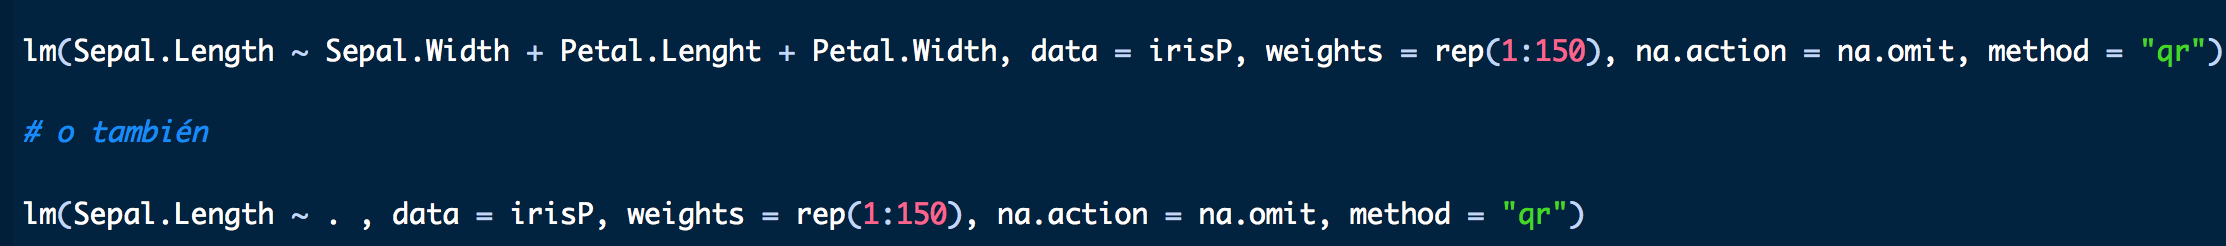
\includegraphics{images/reg19.png}
\caption{\label{fig:"R2"}}
\end{figure}

Si hacemos uso del código anterior obtendremos la información básica del modelo, la cual se presenta en la siguiente imagen:

\begin{figure}
\centering
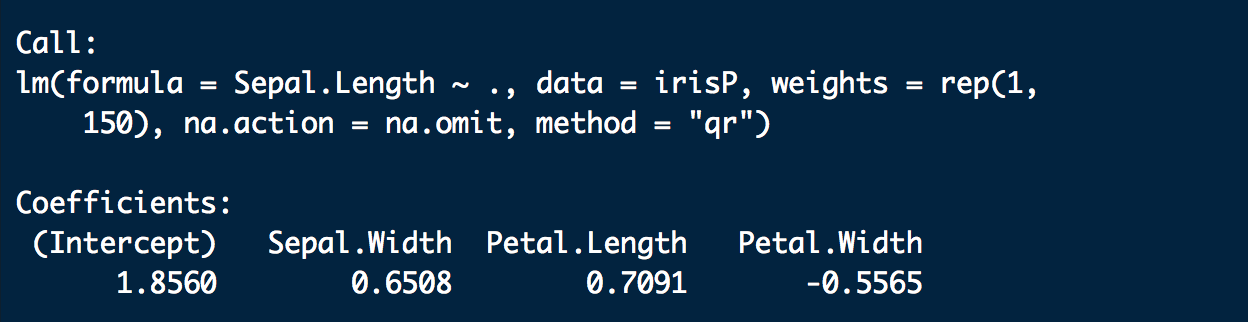
\includegraphics{images/reg20.png}
\caption{\label{fig:"R2"}}
\end{figure}

En esta imagen se nos proporciona el valor que se introdujo en el modelo y los coeficientes de la regresión. Si queremos los datos del modelo usamos la función \emph{summary()}

\begin{figure}
\centering
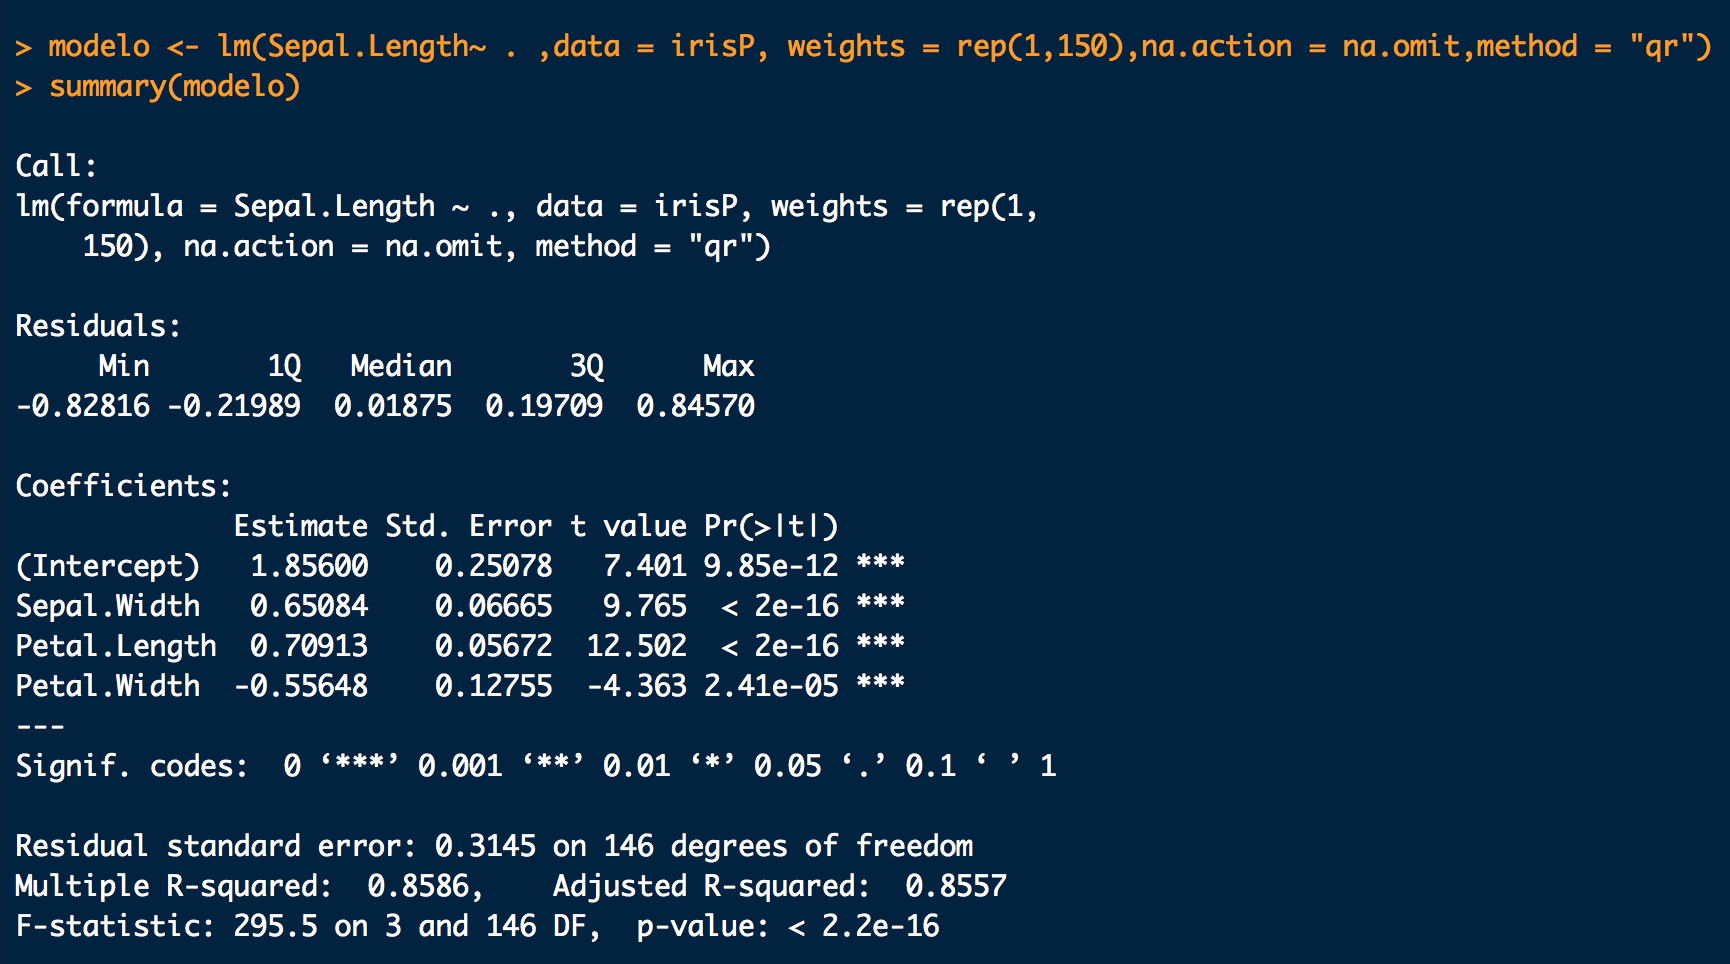
\includegraphics{images/reg23.png}
\caption{\label{fig:"R2"}}
\end{figure}

\hypertarget{aplicando-el-modelo-de-regresion-lineal-en-python}{%
\subsection{\texorpdfstring{Aplicando el modelo de regresión lineal en \emph{Python}:}{Aplicando el modelo de regresión lineal en Python:}}\label{aplicando-el-modelo-de-regresion-lineal-en-python}}

Existen varias librerías para aplicar modelos lineales en \emph{Python}, entre las más populares están \emph{StatsModels} y \emph{sklearn}. Usaremos la primera por ser la que nos proporciona unas funciones parecidas a las que tenemos en \emph{R}. Como el objetivo de este curso es aprender a usar la herramienta, no incluiremos algunos parámetros como los que describimos en \emph{R}.

Para crear el modelo usando la librería \emph{StatsModels}, debemos importar la librería de la manera usual. Luego seleccionamos la variable dependiente e independientes, a diferencia de \emph{R}, \emph{StatsModel} no calcula el valor del intercept por defecto, por lo tanto debemos especificarlo de manera explícita. Esto lo hacemos con la función \emph{add\_constant()} de la misma librería, luego usando la función \emph{.OLS()} para crear el modelo y la función \emph{.fit()} para entrenarlo. Finalmente imprimimos los datos del modelo usando la función \emph{.summary()}

\begin{figure}
\centering
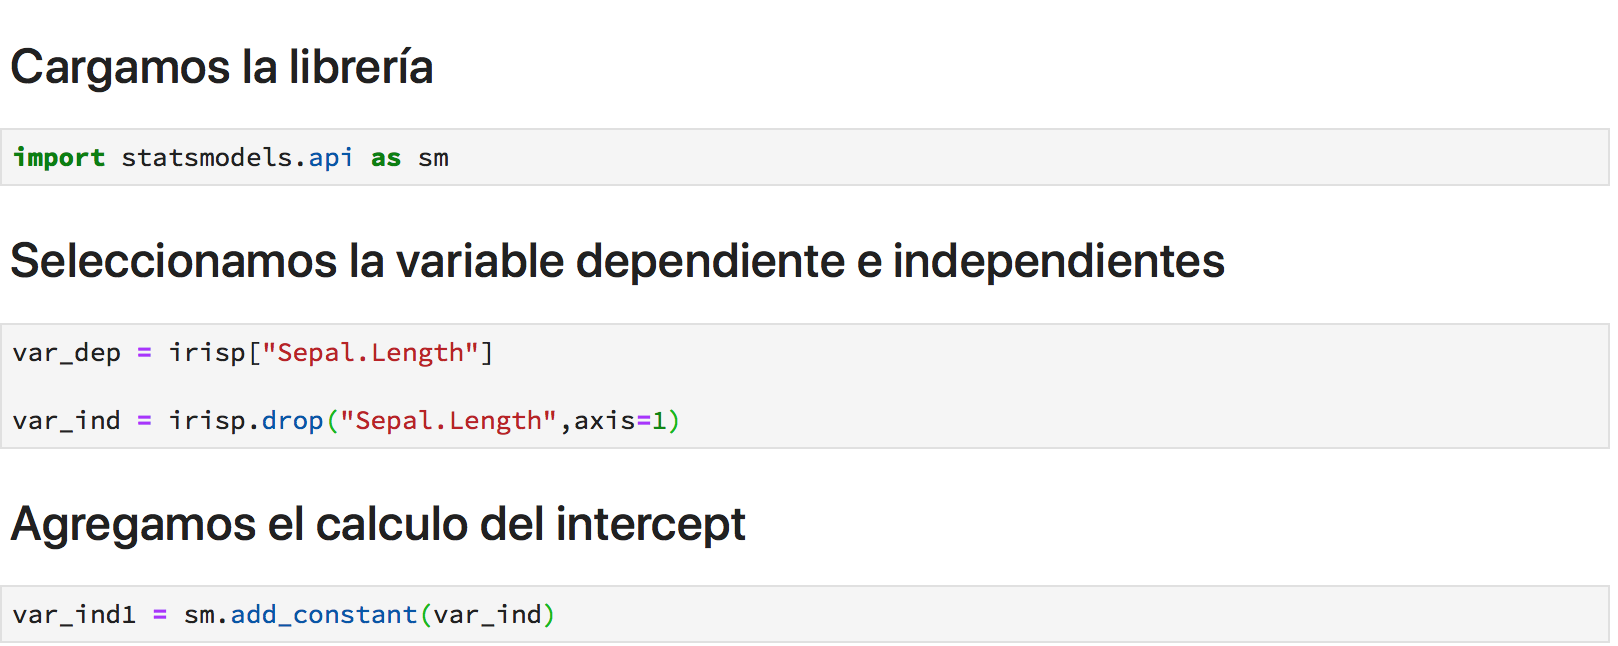
\includegraphics{images/reg21.png}
\caption{\label{fig:"R2"}}
\end{figure}

\begin{figure}
\centering
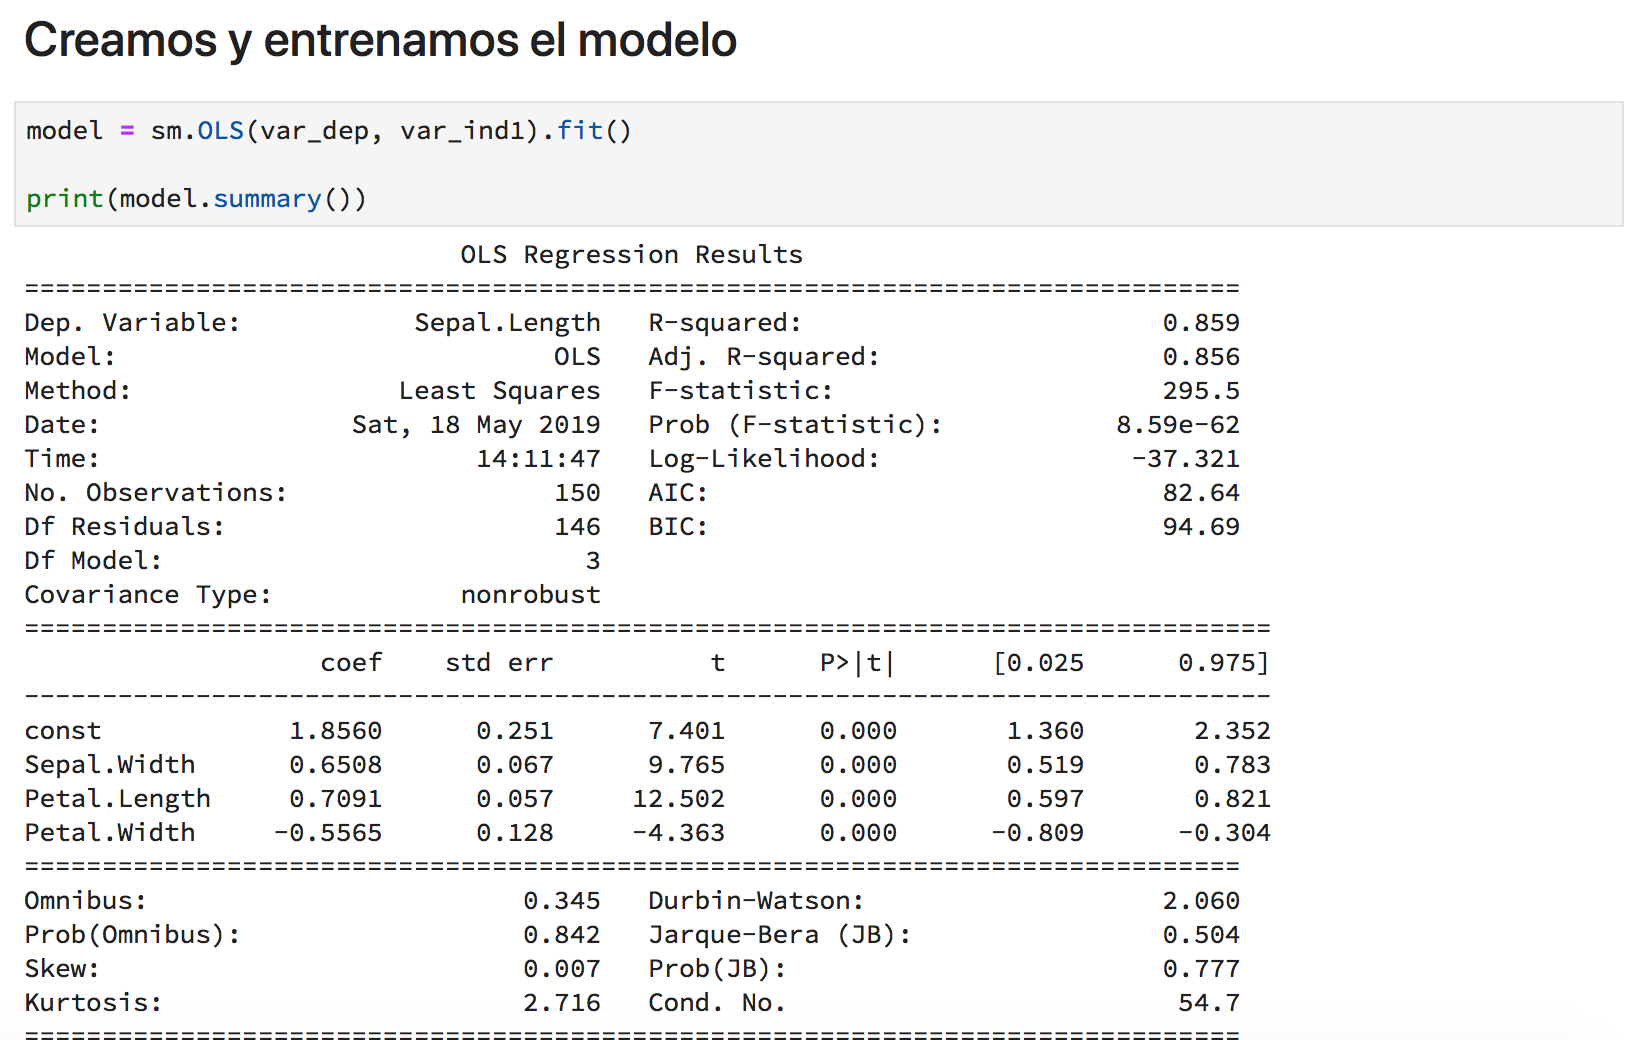
\includegraphics{images/reg22.png}
\caption{\label{fig:"R2"}}
\end{figure}

\hypertarget{como-interpretar-los-resultados-del-modelo}{%
\section{Cómo interpretar los resultados del modelo}\label{como-interpretar-los-resultados-del-modelo}}

Ya vimos que una vez construido el modelo usando funciones con el nombre de \emph{summary} obtenemos información sobre características de los modelos. Describiremos las más importantes y como entender su efecto en el modelo.

\hypertarget{interpretar-con-summary-en-r}{%
\subsection{\texorpdfstring{Interpretar con \emph{summary} en \emph{R}:}{Interpretar con summary en R:}}\label{interpretar-con-summary-en-r}}

\begin{itemize}
\tightlist
\item
  \emph{residuals}: Al calcular el modelo, la función \emph{summary} calcula las predicciones para los mismos datos con los que se entrenó el modelo y la variable \emph{residuals} nos da los errores de predicción. Con esta variable se pueden obtener el menor, el mayor, la mediana, primer cuantil y tercer cuantil de los errores. Debemos realizar un histograma de los errores del modelo, si este histograma es distinto a un comportamiento normal, debemos pensar rápidamente que nuestro modelo es inadecuado. A continuación se muestra el código y un histograma ideal, suponiendo que usamos el ``modelo'' obtenido en la sección anterior
\end{itemize}

\begin{figure}
\centering
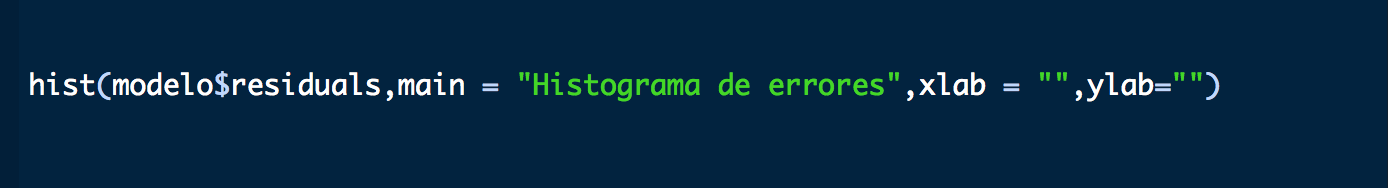
\includegraphics{images/reg25.png}
\caption{\label{fig:"R2"}}
\end{figure}

\begin{figure}
\centering
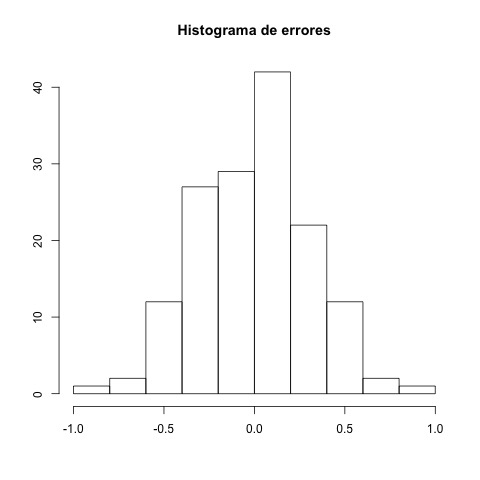
\includegraphics{images/reg24.jpeg}
\caption{\label{fig:"R2"}}
\end{figure}

\begin{itemize}
\item
  \emph{Coefficients}: Luego se muestran los coeficientes del modelo en forma de matriz:

  \begin{itemize}
  \tightlist
  \item
    En la primera columna se muestran los coeficientes del modelo.
  \item
    En la segunda columna se muestran las desviaciones estándares de cada coeficiente.
  \item
    Luego se muestran los valores correspondientes al estadístico \(t\), con el fin de realizar una prueba de hipótesis a los coeficientes.
  \item
    En cuarta columna se muestran los \(p\)-valores de la prueba de hipótesis, los resultados de estos valores deben ser lo más pequeños posibles, en general, se esperan que sean menores a 0.05, en caso de que esto no ocurra, debemos pensar en eliminar la variable del modelo, o realizar alguna transformación adecuada.
  \end{itemize}
\item
  \emph{Residual standard error}: Nos da una idea de cómo varía el error de precisión del modelo, es decir, nos dice como varían las predicciones de las observaciones.
\item
  \emph{Multiple R-squared} and \emph{Adjusted R-squared} : En ambos casos ambas valores explican el valor de la varianza explicada del modelo. Se diferencian en que el segundo parámetro considera el número de variables involucradas en el modelo, por lo cual en la mayoría de los casos se utiliza con preferencia sobre el primero y se buscan valores mayores a 0.7 o 0.8.
\item
  \emph{\(F\)-statistic}: Nos presenta el valor del estadístico \(F\), luego los grados de libertad y por último el \(p\)-valor de la prueba de hipótesis que resulta de contrastar el modelo resultante con el modelo que únicamente consta de un término intercept
\end{itemize}

\hypertarget{interpretar-con-summary-en-python}{%
\subsection{\texorpdfstring{Interpretar con \emph{summary} en \emph{Python}}{Interpretar con summary en Python}}\label{interpretar-con-summary-en-python}}

El \emph{summary} en este caso nos da mucha más información que en \emph{R}. Nos concentraremos en las mismas variables del \emph{summary} y mencionaremos algunas otras que pueden ser de utilidad. Este \emph{summary} se divide en dos cuadros:

\begin{itemize}
\item
  Información estadística del modelo: en esta primera matriz la información más relevante es el nombre de la variable dependiente, el número de observaciones, \emph{Multiple R-squared}, \emph{Adjusted R-squared} y el valor de \emph{\(F\)-statistic}
\item
  Información estadística acerca de los coeficientes del modelo: en esta matriz se encuentra prácticamente la misma información concerniente a los valores de los coeficientes del modelo, con la información extra que consiste en los intervalos de confianza de los coeficientes.
\item
  Este \emph{summary} no aporta información clara sobre los residuos del modelo. Para poder obtener un histograma y ver su comportamiento usamos el siguiente código, recordando que nuestro modelo se llama ``modelo'':
\end{itemize}

\begin{figure}
\centering
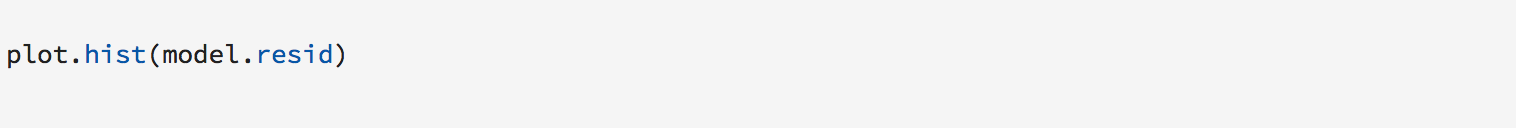
\includegraphics{images/reg26.png}
\caption{\label{fig:"R2"}}
\end{figure}

\hypertarget{realizando-predicciones-con-nuestro-modelo}{%
\section{Realizando predicciones con nuestro modelo}\label{realizando-predicciones-con-nuestro-modelo}}

El objetivo principal de crear modelos es usarlos para predecir valores a partir de las variables independientes. A continuación presentaremos los códigos para realizar dicha predicción:

\hypertarget{realizando-predicciones-con-r}{%
\subsection{\texorpdfstring{Realizando predicciones con \emph{R}}{Realizando predicciones con R}}\label{realizando-predicciones-con-r}}

Para realizar predicciones con \emph{R} haremos uso de la función \emph{predict()}. Debemos ser cuidadosos con los conjuntos de datos que usaremos para predecir, estos datos deben tener las columnas con el mismo nombre y no tener valores faltantes o espacios en blanco. A continuación se anexa el código para hacer la predicción.

\begin{figure}
\centering

\includegraphics{images/reg27.png}
\caption{\label{fig:"R2"}}
\end{figure}

\hypertarget{realizando-predicciones-con-python}{%
\subsection{\texorpdfstring{Realizando predicciones con \emph{Python}}{Realizando predicciones con Python}}\label{realizando-predicciones-con-python}}

Al realizar predicciones en \emph{Python} debemos tener en claro el orden del conjunto de datos, es decir, debemos tener las variables independientes en el mismo orden con el que se entrenó el modelo, además, debemos agregar una variable intercept para que el modelo tenga todos los parámetros requeridos.

\begin{figure}
\centering
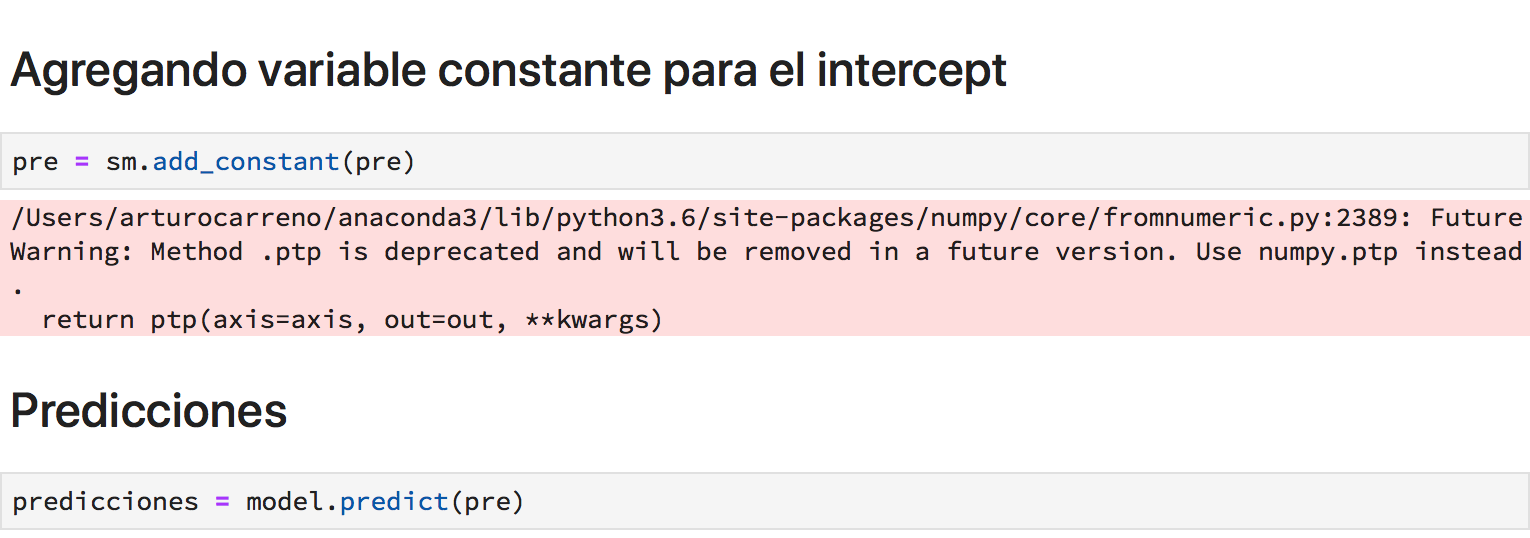
\includegraphics{images/reg28.png}
\caption{\label{fig:"R2"}}
\end{figure}

\hypertarget{regresion-logistica}{%
\chapter{Regresión logística}\label{regresion-logistica}}

La regresión logística nos da respuesta a la siguiente interrogante, ¿Qué hacer cuando la variable dependiente es dicotómica? Claramente en los modelos lineales esto es inaplicable pues la variable dependiente debe ser continua. De igual manera la otra interrogante importante es ¿Qué hacer cuando las variables independientes son categóricas? La regresión logística da la flexibilidad necesaria para incluir este tipo de variables. La regresión logística calcula la probabilidad de que el evento ocurra, y en esto se diferencia de la regresión lineal en la cual se calculaba directamente el valor de la variable. Por ejemplo, si estamos interesados en el evento cara o cruz, un modelo logístico para este tipo de modelos nos dará la probabilidad de que ocurra cara o cruz.

\hypertarget{supuestos-de-la-regresion-logistica}{%
\section{Supuestos de la regresión logística}\label{supuestos-de-la-regresion-logistica}}

La regresión logística es flexible con respecto a supuestos como normalidad o la continuidad de las variables. Una de las hipótesis que debemos verificar es la inexistencia de multicolinealidad entre las distintas variables continuas y la correlación entre las variables independientes y la variable dependiente. A continuación veremos cómo responder a estas interrogantes.

\hypertarget{multicolinealidas-entre-variables-independientes}{%
\section{Multicolinealidas entre variables independientes}\label{multicolinealidas-entre-variables-independientes}}

Al igual que en la regresión lineal debemos evitar variables independientes con alta correlación. Para ello debemos realizar el mismo procedimiento visto en el capítulo anterior.

\hypertarget{detectar-correlacion-entre-variables-categoricas}{%
\section{Detectar correlación entre variables categóricas}\label{detectar-correlacion-entre-variables-categoricas}}

Una de las primeras cosas que debemos revisar es la independencia entre las variables independientes categóricas y la dependencia entre la variable dependiente y las variables categóricas independientes. Para ello haremos uso de las tablas de contingencia.

Una tabla de contingencia es la forma más fácil de detectar relaciones entre variables categóricas, en estas tablas se definen las variables en filas y columnas y se ven las distintas proporciones entre las categorías de las variables. En la siguiente imagen se muestra un ejemplo de tabla de contingencia

\begin{figure}
\centering
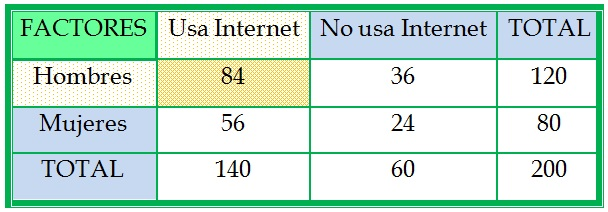
\includegraphics{images/log.jpg}
\caption{\label{fig:"R2"}}
\end{figure}

En las columnas la variable hace referencia al uso del internet y en las filas las variables hacen referencia al sexo.

Para detectar si dos variables están o no correlacionadas usaremos la prueba \emph{chi-cuadrado} que contrasta la independencia entre las variables, es decir, si el \emph{\(p\)-valor} es bajo estamos encontrando evidencia de independencia entre los factores, en caso contrario podemos suponer la existencia de cierta relación entre las variables.

En la siguiente imagen se muestra una tabla de contingencia, a la cual le aplicaremos la prueba \emph{chi-cuadrado}, para contrastar la independencia entre el uso de internet y el estar empleado. La tabla se construye con el siguiente código:

\begin{figure}
\centering
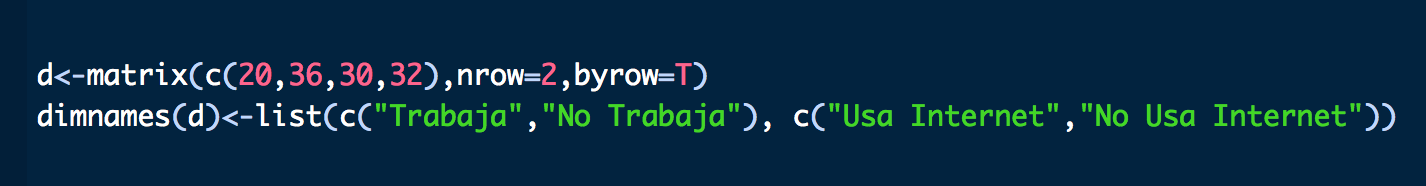
\includegraphics{images/log2000.png}
\caption{\label{fig:"R2"}}
\end{figure}

\begin{figure}
\centering
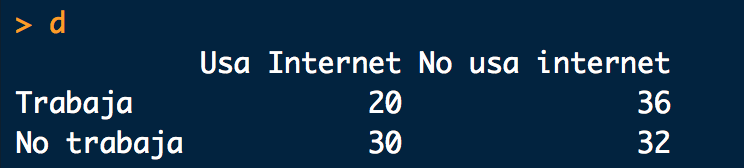
\includegraphics{images/log2.png}
\caption{\label{fig:"R2"}}
\end{figure}

\hypertarget{prueba-chi-cuadrado-en-r}{%
\subsection{\texorpdfstring{Prueba chi-cuadrado en \emph{R}}{Prueba chi-cuadrado en R}}\label{prueba-chi-cuadrado-en-r}}

Para realizar la prueba usamos la función \emph{chisq.test()} y obtenemos el siguiente resultado

\begin{figure}
\centering
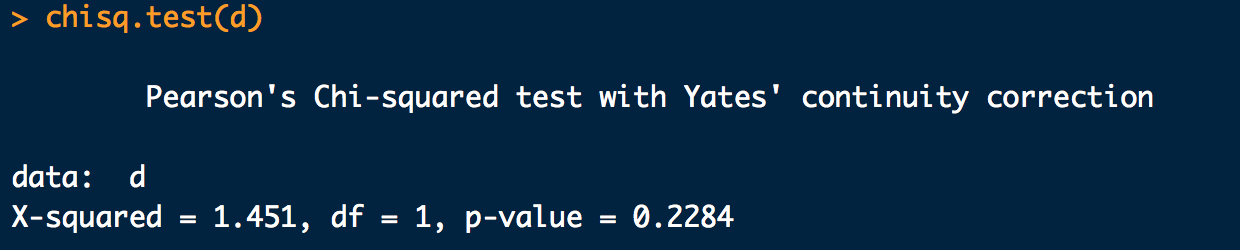
\includegraphics{images/log3.png}
\caption{\label{fig:"R2"}}
\end{figure}

El valor que interesa es el \emph{\(p\)-valor}, el cual al ser mayor a 0.05 indica una posible relación entre las variables. En general, si el \emph{\(p\)-valor} es cercano a uno podemos pensar en una posible relación entre las variables.

\hypertarget{prueba-chi-cuadrado-en-python}{%
\subsection{\texorpdfstring{Prueba chi-cuadrado en \emph{Python}}{Prueba chi-cuadrado en Python}}\label{prueba-chi-cuadrado-en-python}}

Para realizar la prueba \emph{chi-cuadrado} en Python usaremos la librería \emph{scipy} y usaremos la función \emph{.chi2\_contingency()}. A continuación mostramos como hacerlo

\begin{figure}
\centering
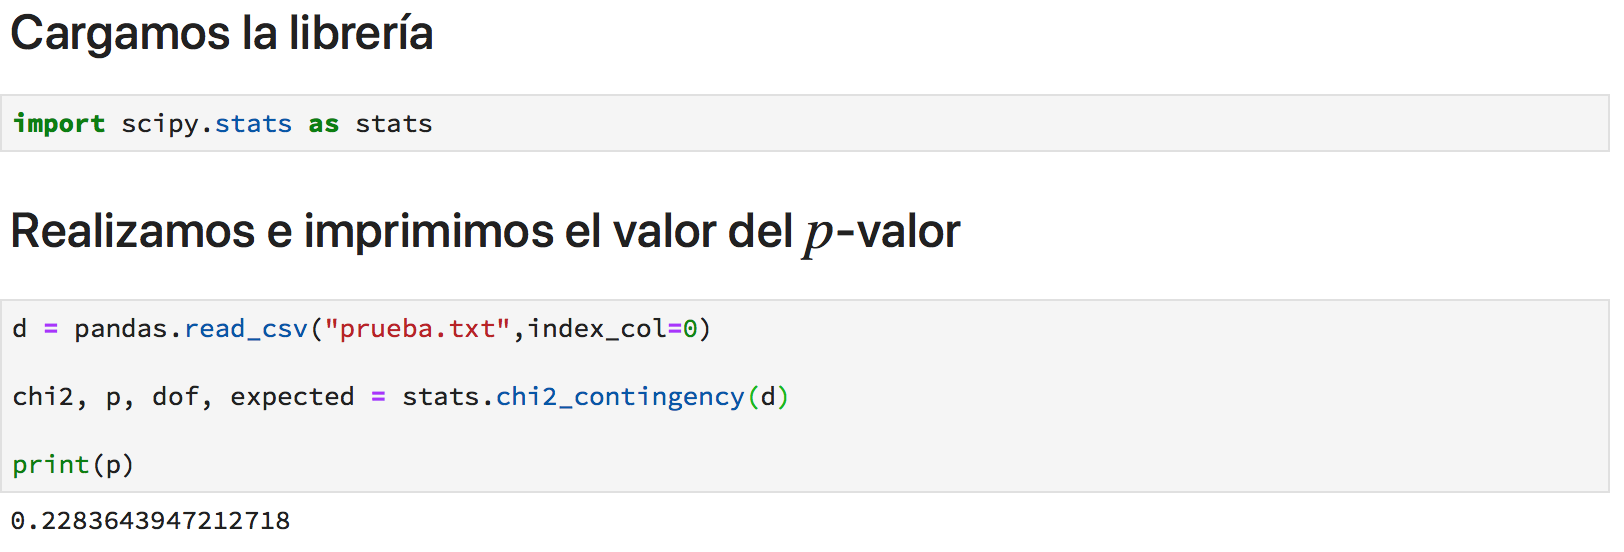
\includegraphics{images/log4.png}
\caption{\label{fig:"R2"}}
\end{figure}

\hypertarget{detectar-correlacion-entre-variables-categoricas-y-variables-cuantitativas}{%
\section{Detectar correlación entre variables categóricas y variables cuantitativas}\label{detectar-correlacion-entre-variables-categoricas-y-variables-cuantitativas}}

Para detectar un posible efecto entre la correlación de una variable categórica y una variable continua usaremos un estadístico llamado \emph{\(d\) de Cohen}, el cual se construye a partir de las diferencias de las medias de la segmentación a través de la variable categórica. Dependiendo del valor del estadístico diremos si existe o no un efecto de la variable categórica y la variable cuantitativa. En general si el valor es menor 0.5 diremos que hay un efecto débil, si el valor está entre 0.5 y 0.8 diremos que hay un efecto moderado y si es mayor a 0.8 diremos que hay un efecto fuerte. En general este estadístico es útil cuando la variable categórica posee dos categorías, en otro caso, el estadístico pierde utilidad y se suele usar una herramienta estadística conocida como \emph{Anova}, la cual veremos en otro curso.

\hypertarget{medida-de-d-de-cohen-en-r}{%
\subsection{\texorpdfstring{Medida de \(d\) de Cohen en \emph{R}}{Medida de d de Cohen en R}}\label{medida-de-d-de-cohen-en-r}}

Deberemos instalar la librería \emph{effsize} y usaremos la función \emph{cohen.d()}, además crearemos una variable artificial para mostrar el uso del estadístico:

\begin{figure}
\centering
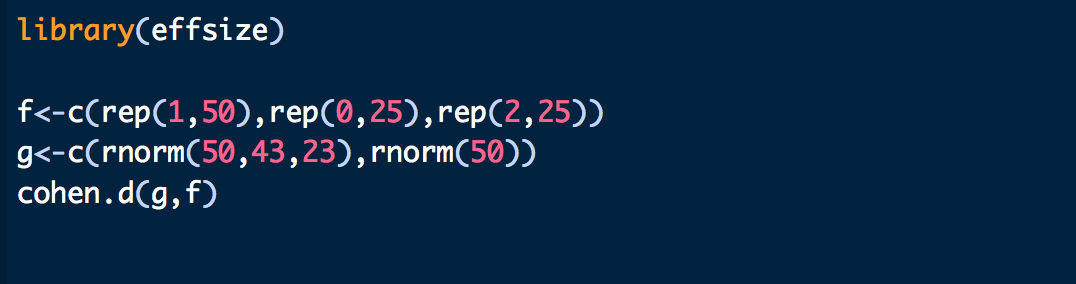
\includegraphics{images/log5.png}
\caption{\label{fig:"R2"}}
\end{figure}

\begin{figure}
\centering
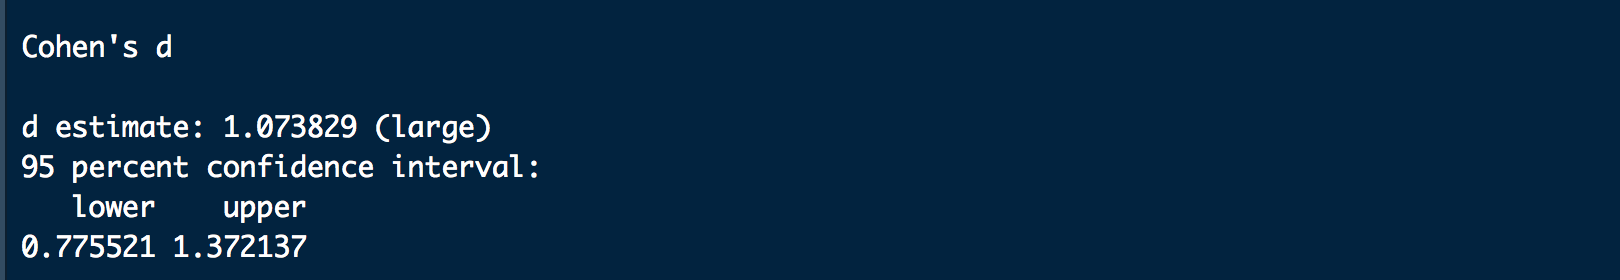
\includegraphics{images/log6.png}
\caption{\label{fig:"R2"}}
\end{figure}

Podemos notar que el valor del estadístico \emph{\(d\) de Cohen} es alto mostrando un posible efecto de las variables categóricas en la variable continua.

\hypertarget{medida-de-d-de-cohen-en-python}{%
\subsection{\texorpdfstring{Medida de \(d\) de Cohen en \emph{Python}}{Medida de d de Cohen en Python}}\label{medida-de-d-de-cohen-en-python}}

En \emph{Python} no existe una función para calcular la \emph{\(d\) de Cohen} de manera directa por lo que tendremos que programarla por nuestra cuenta, para ello usaremos las librerías \emph{statistics} y \emph{math} las cuales nos permitirán calcular las métricas que necesita el estadístico de \emph{Cohen}.

\begin{figure}
\centering
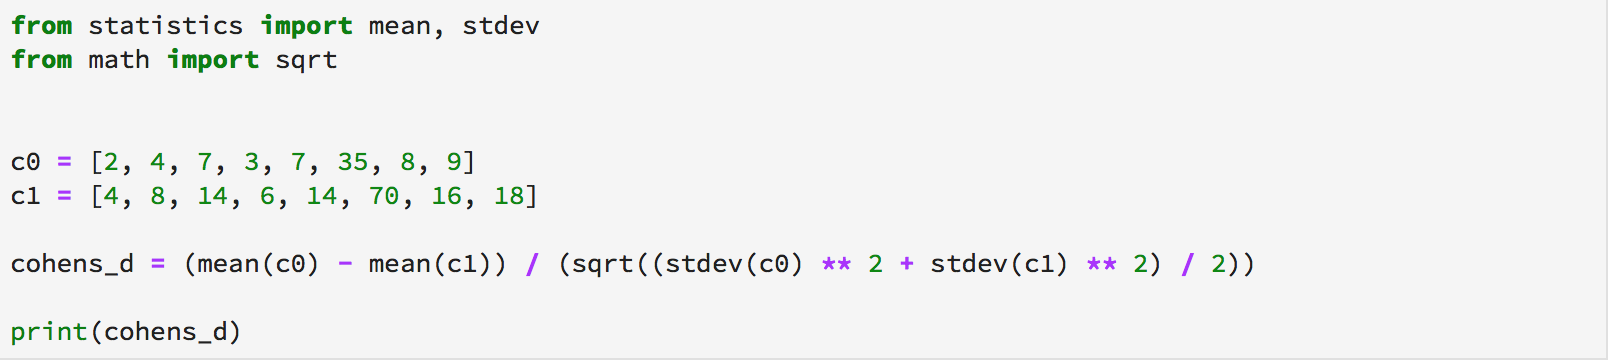
\includegraphics{images/log7.png}
\caption{\label{fig:"R2"}}
\end{figure}

\hypertarget{codificando-variables-categoricas}{%
\section{Codificando variables categóricas}\label{codificando-variables-categoricas}}

Una variable categórica no puede ser ingresada directamente al modelo, pues se asume que es una variable continua, por lo cual arrojará una interpretación errónea del comportamiento de la variable. El procedimiento estándar es crear variables auxiliares binarias que nos indiquen la presencia o no de cierto atributo. Por ejemplo, si tenemos una variable categórica con tres categorías: rojo, azul y verde, debemos crear dos variables auxiliares: la primera que esté compuesta por 0 si es roja, 1 si no, la segunda que esté compuesta por 1 si es azul 0 si no. Es innecesario crear una tercera variable para el color verde, pues se entiende que si las primeras variables son 0 y 0, se concluye que debe ser verde. En general si una variable categórica está compuesta por \(n\) categorías debemos crear \(n-1\) variables auxiliares, en algunas fuentes esto también se conoce como creación de variables \emph{Dummies}

\hypertarget{creacion-de-variables-auxiliares-en-r}{%
\subsection{\texorpdfstring{Creación de variables auxiliares en \emph{R}}{Creación de variables auxiliares en R}}\label{creacion-de-variables-auxiliares-en-r}}

Debemos descargar y usar la librería \emph{fastDummies}, la cual tiene la función del mismo nombre \emph{dummy\_cols()}. Esta función es la que crea las variables auxiliares. Por ejemplo, supongamos que tenemos la variable color, la cual está compuesta por: (``azul'',``rojo'',``amarillo'',``blanco'',``amarillo'', ``azul'',``azul'',``rojo''), en la cual tenemos 4 categorías. Para aplicar la función \emph{dummy\_cols()} realizaremos el siguiente código:

\begin{figure}
\centering

\includegraphics{images/log8.png}
\caption{\label{fig:"R2"}}
\end{figure}

Y obtenemos como resultado:

\begin{figure}
\centering
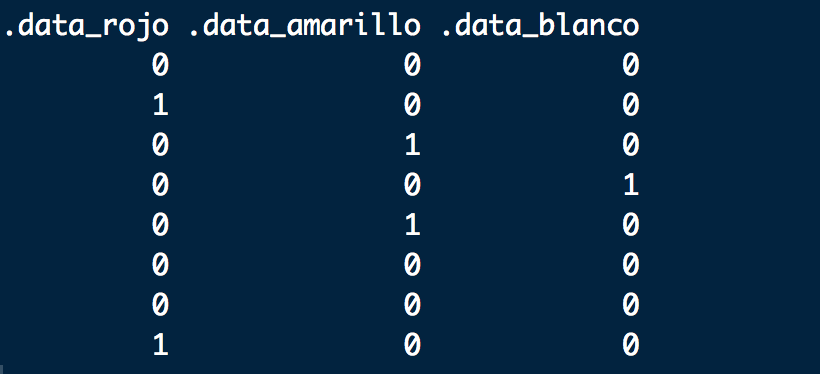
\includegraphics{images/log9.png}
\caption{\label{fig:"R2"}}
\end{figure}

Observamos que en el séptimo registro tenemos una fila de números ceros, por lo ya señalado esto significa que el atributo de esta observación es azul.

\hypertarget{creacion-de-variables-auxiliares-en-python}{%
\subsection{\texorpdfstring{Creación de variables auxiliares en \emph{Python}}{Creación de variables auxiliares en Python}}\label{creacion-de-variables-auxiliares-en-python}}

Para crear variables auxiliares en \emph{Python}, utilizaremos función \emph{get\_dummies()} del paquete Pandas. A continuación mostramos el código y el resultado.

\begin{figure}
\centering
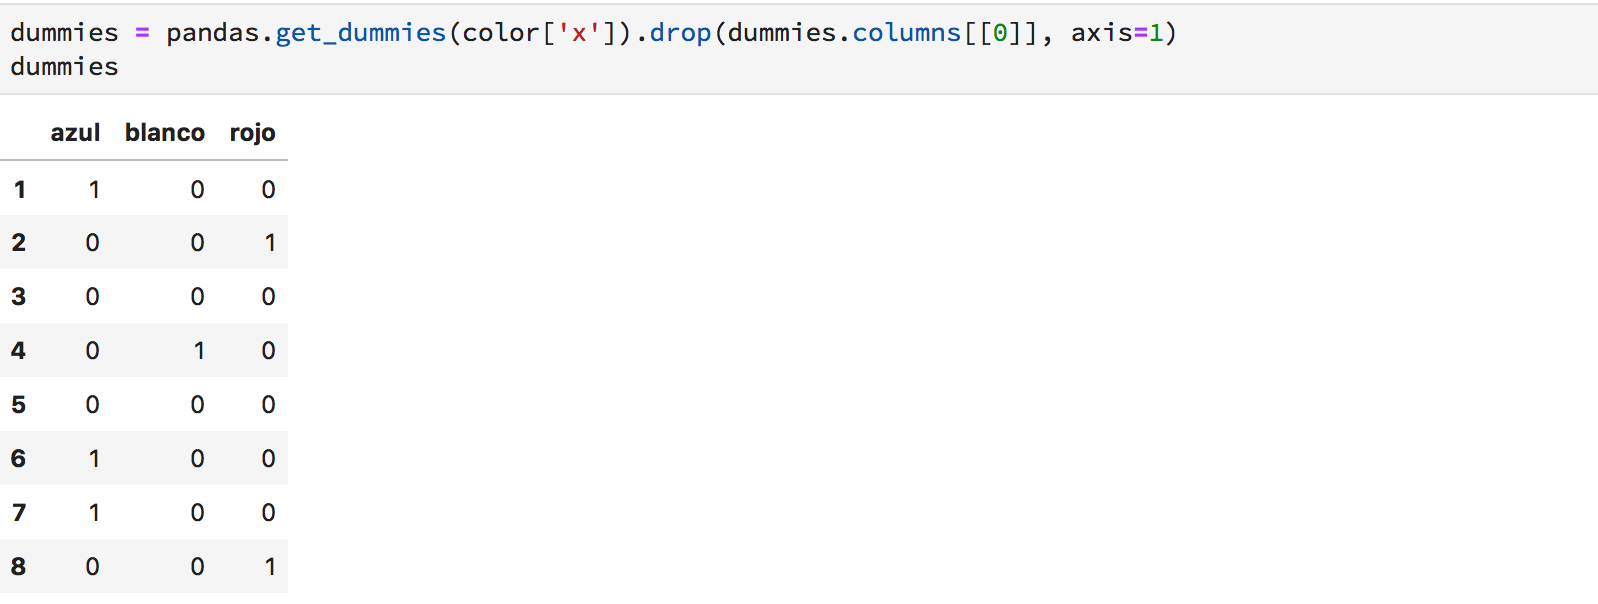
\includegraphics{images/log10.png}
\caption{\label{fig:"R2"}}
\end{figure}

\hypertarget{aplicando-el-modelo-de-regresion-logistica}{%
\section{Aplicando el modelo de regresión logística}\label{aplicando-el-modelo-de-regresion-logistica}}

Una vez realizado un paseo por los pasos anteriores debemos proceder a realizar la construcción del modelo como tal. Iniciaremos con el lenguaje \emph{R}:

\hypertarget{modelo-logistico-en-r}{%
\subsection{Modelo logístico en R}\label{modelo-logistico-en-r}}

Para el cálculo del modelo logístico haremos uso de la función \emph{glm()} que está disponible como función base en R. Esta función tiene prácticamente la misma sintaxis que la función \emph{lm()}, así que no describiremos en detalle sus parámetros.

Usaremos los datos \emph{Default} (incumplimiento) que nos proporciona el paquete \emph{ISLR} sobre registros de clientes con incumplimiento de pagos de una empresa de tarjetas de crédito, los cuales podemos observar en la siguiente imagen:

\begin{figure}
\centering

\includegraphics{images/log110.png}
\caption{\label{fig:"R2"}}
\end{figure}

\begin{figure}
\centering
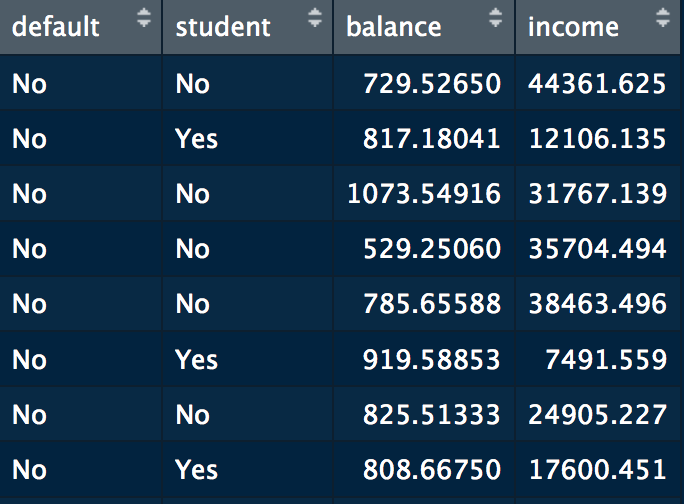
\includegraphics{images/log11.png}
\caption{\label{fig:"R2"}}
\end{figure}

Si queremos crear un modelo logístico para predecir el incumplimiento de pago de los estudiantes que tenga variables independientes \emph{balance}, \emph{income} y variable dependiente \emph{default} debemos usar el siguiente código

\begin{figure}
\centering
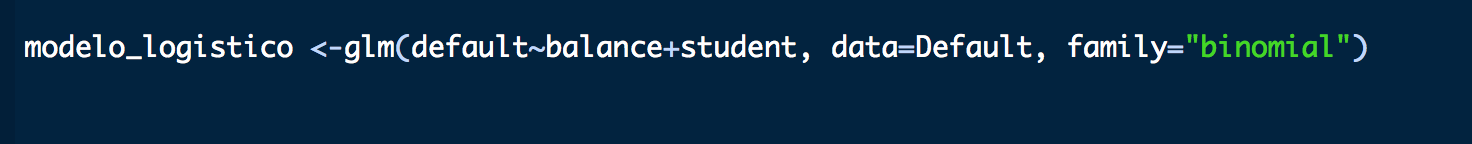
\includegraphics{images/log12.png}
\caption{\label{fig:"R2"}}
\end{figure}

tenemos un parámetro adicional llamado \emph{Family} el cual hace referencia a la distribución de la variable que en nuestro caso es la binomial.

Al realizar un resumen del modelo con la función \emph{summary}, obtenemos:

\begin{figure}
\centering
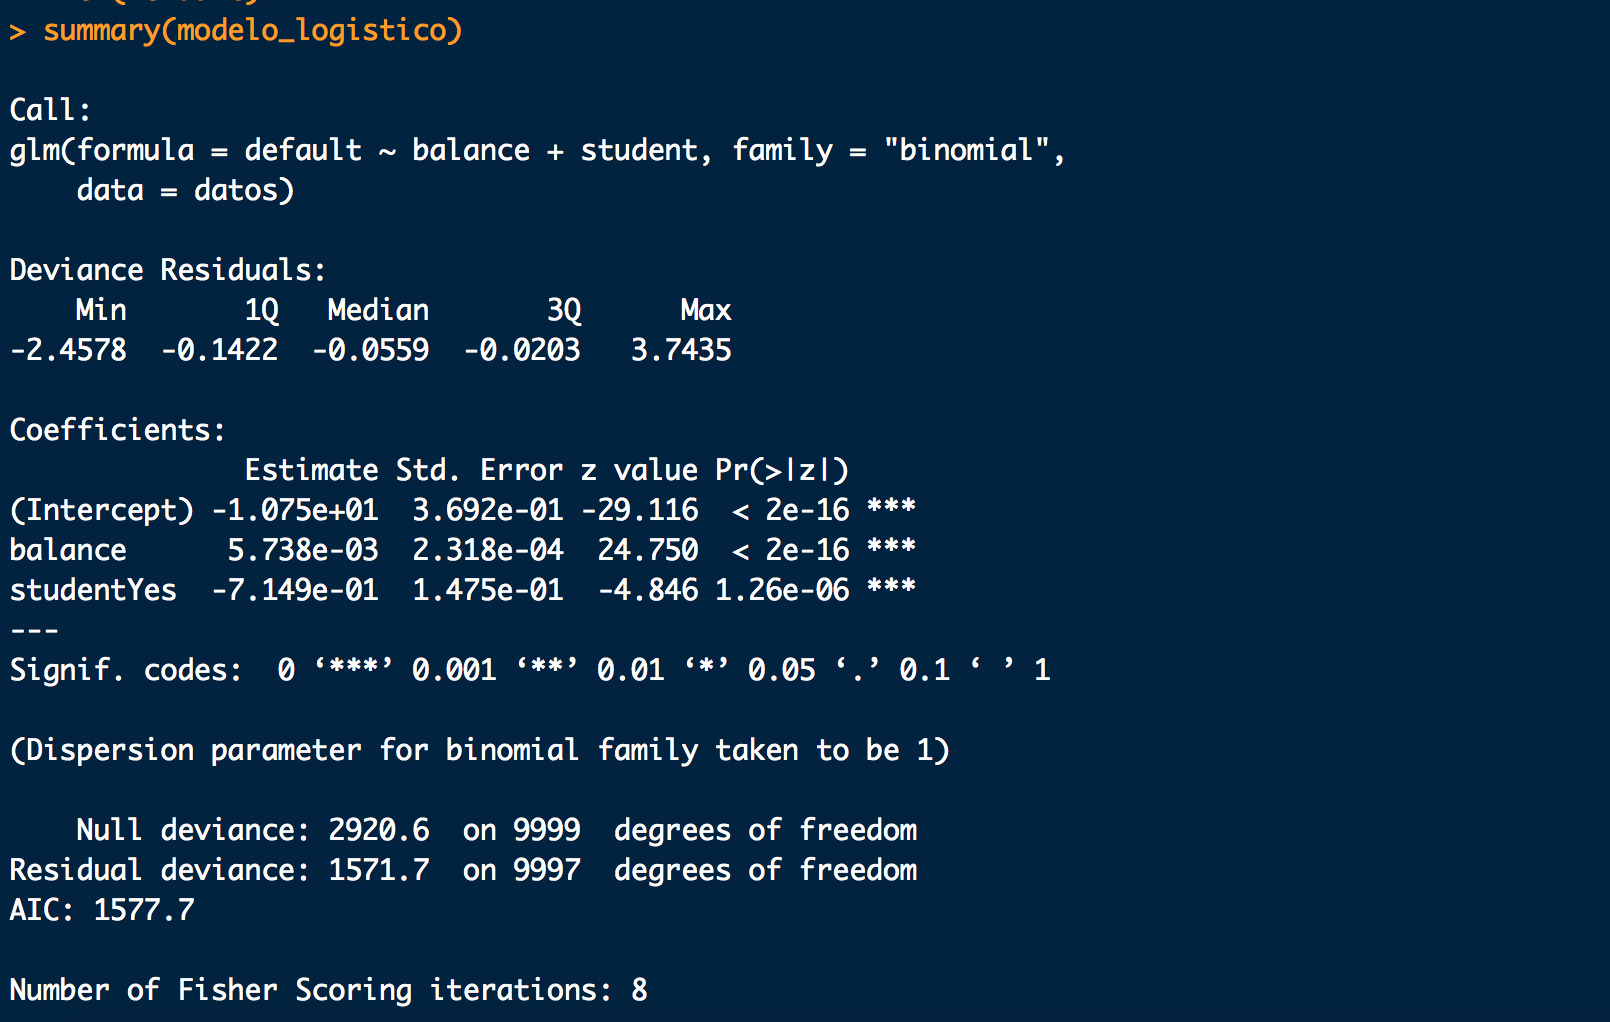
\includegraphics{images/log13.png}
\caption{\label{fig:"R2"}}
\end{figure}

La imagen anterior es una presentación del resumen del modelo un poco diferente a la del capítulo anterior. Vale la pena describir la variable \emph{AIC}, este estadístico nos da información acerca de la bondad del modelo con respecto a las variables introducidas, es decir, permite comparar distintos modelos estadísticos, buscando un valor lo más pequeño posible de esta variable.

Un error típico en el que se suele caer al crear un modelo de regresión logística es pensar que este modelo dará como predicción alguna variable categórica especifica. En realidad el modelo proporciona la probabilidad de ocurrencia del evento con los datos específicos. Así, la predicción esperada será un número entre 0 y 1.

A continuación presentamos el código para realizar la predicción:

\begin{figure}
\centering
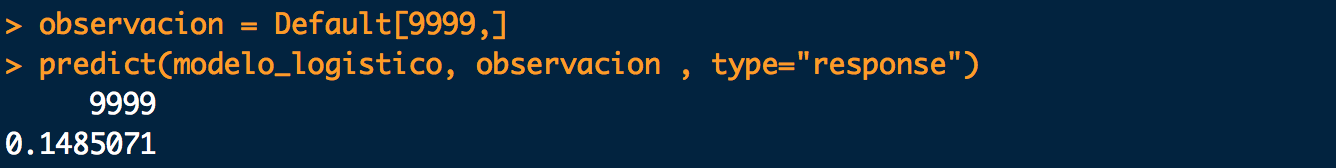
\includegraphics{images/log14.png}
\caption{\label{fig:"R2"}}
\end{figure}

En la imagen anterior el resultado es \(0.14\) significa que la probabilidad de ocurrencia del evento es \(0.14\).

\hypertarget{modelo-logistico-en-python}{%
\subsection{\texorpdfstring{Modelo logístico en \emph{Python}}{Modelo logístico en Python}}\label{modelo-logistico-en-python}}

Para crear el modelo cargaremos la librería \emph{pandas} y \emph{statsmodels}. Usaremos los mismos datos de la parte anterior. A diferencia de \emph{R} debemos separar la variable dependiente de las independientes y verificar que las variables categóricas estén compuestas por valores numéricos. Estos cambios son hechos con la función \emph{.replace()}. Recordemos que por defecto no se calcula la variable intercept en el modelo, por lo cual debemos incorporarla con la función \emph{sm.add\_constant()}. A continuación se muestra este procedimiento:

\begin{figure}
\centering
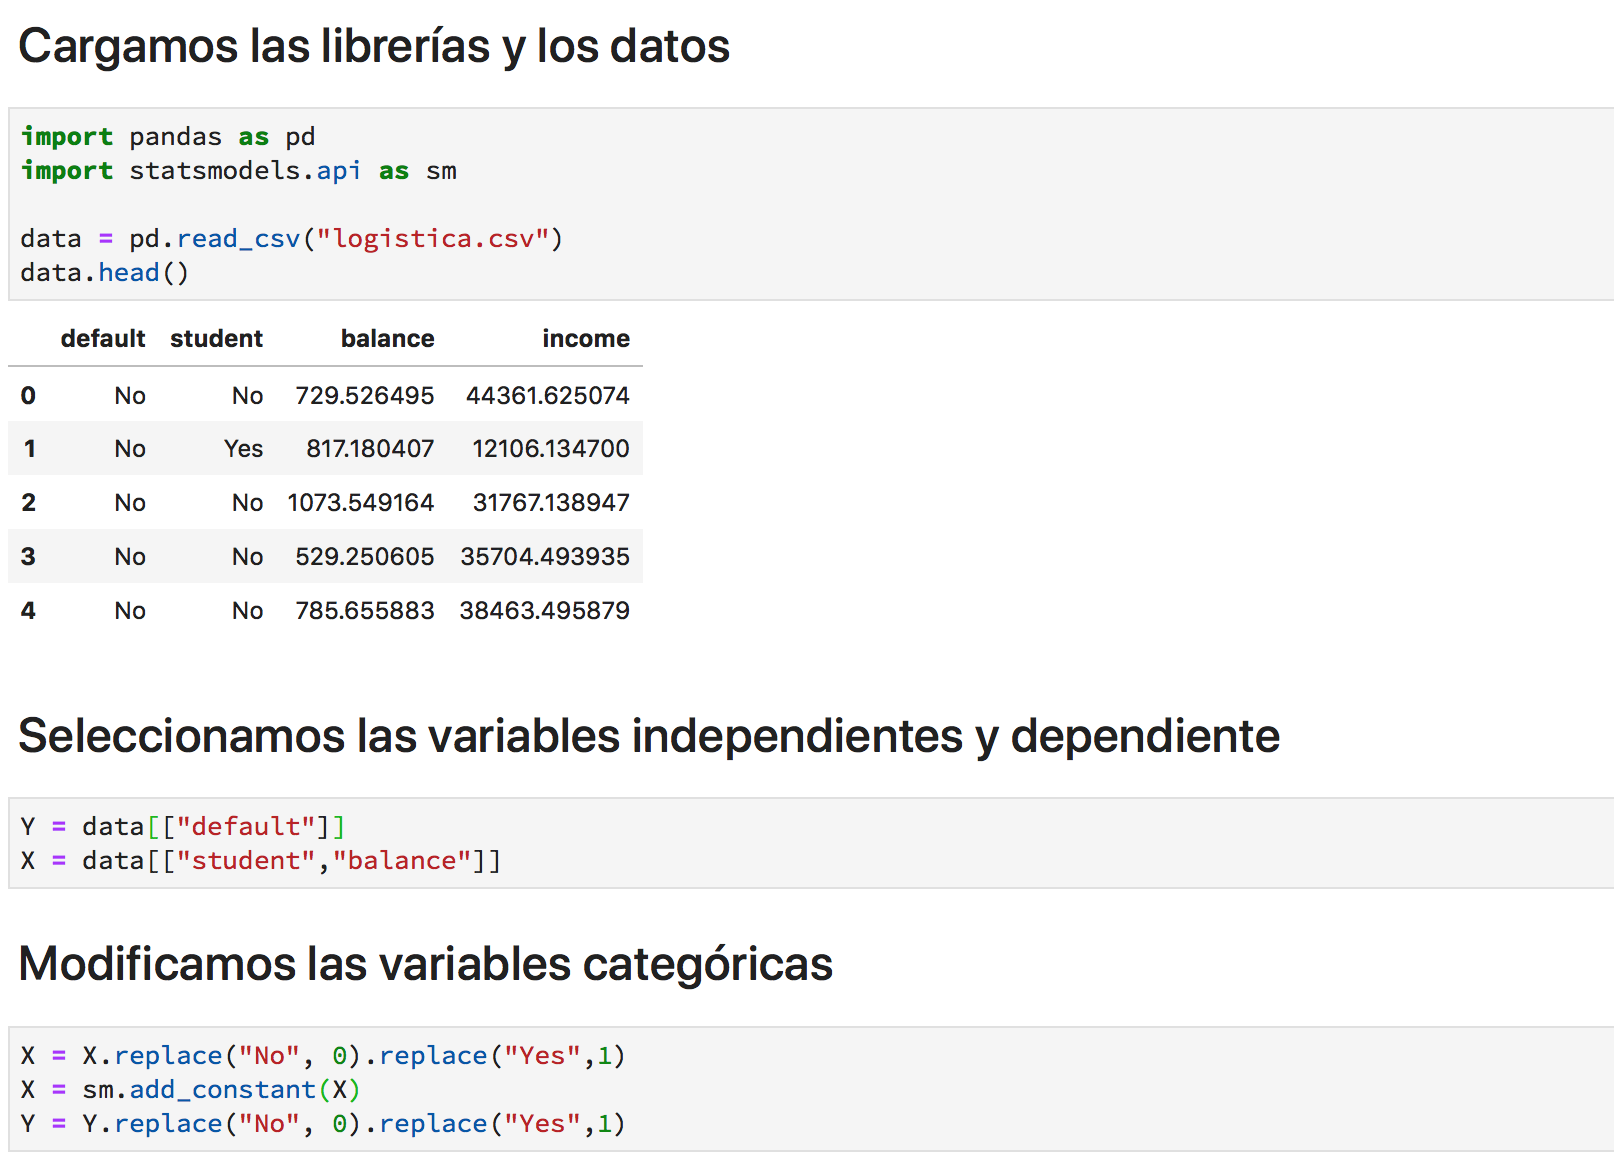
\includegraphics{images/log15.png}
\caption{\label{fig:"R2"}}
\end{figure}

Ahora, procedemos al cálculo del modelo. Primero lo creamos usando la función \emph{sm.logit()} y luego lo entrenamos usando la función \emph{.fit()}. Para ver el resumen del modelo usamos la función \emph{.summary()}, la cual nos da prácticamente la misma información que la función \emph{summary} en \emph{R}.

\begin{figure}
\centering
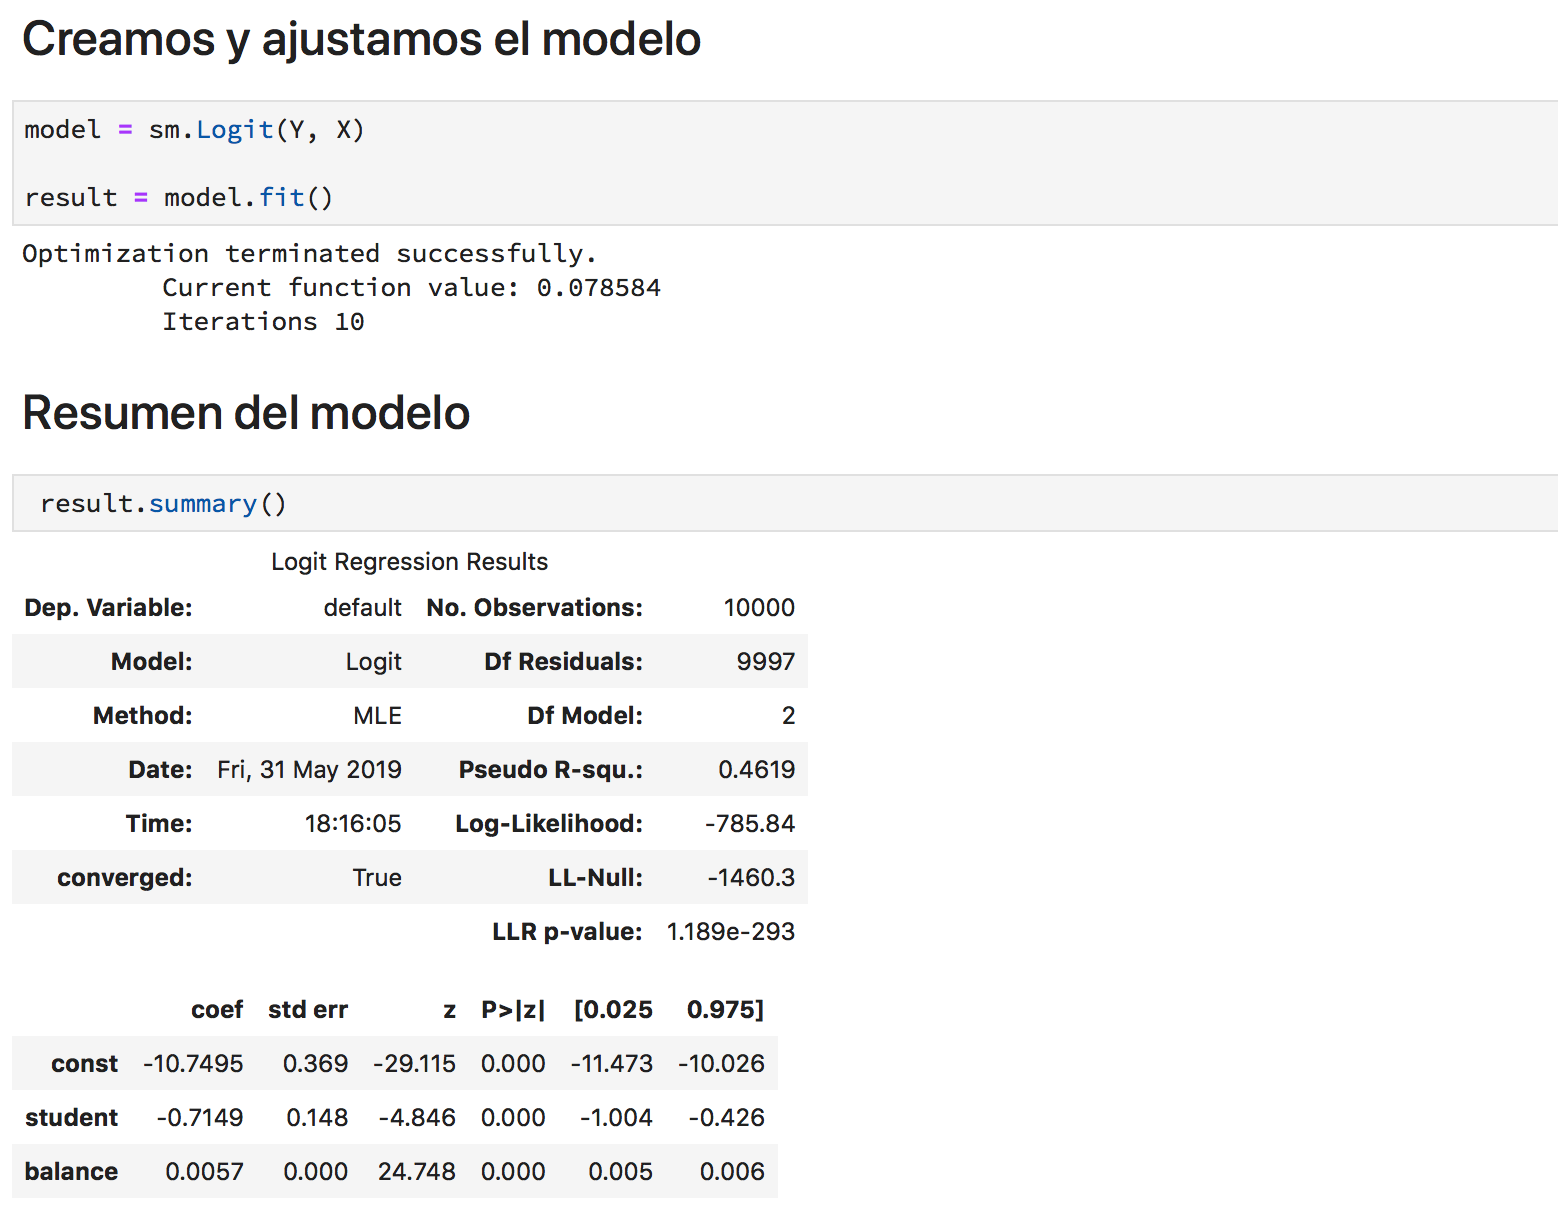
\includegraphics{images/log16.png}
\caption{\label{fig:"R2"}}
\end{figure}

Para concluir, realizamos predicciones usando nuestro modelo, recordando que la observación usada para predecir debe tener la misma estructura de la variable independiente. Debemos tener en cuenta que dependiendo de si se agregó o no el intercept, tendremos que agregar la variable constante usando la función \emph{sm.add\_constant()}. A continuación se muestra este procedimiento:

\begin{figure}
\centering
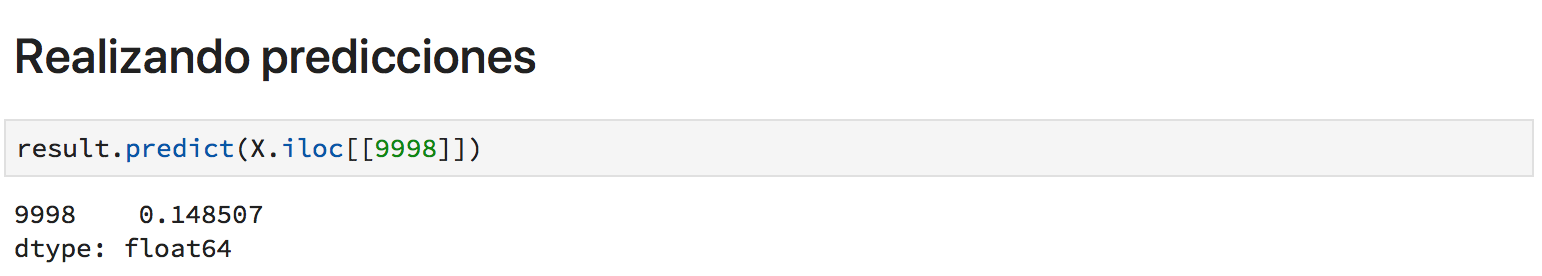
\includegraphics{images/log17.png}
\caption{\label{fig:"R2"}}
\end{figure}

\hypertarget{analisis-de-cluster}{%
\chapter{Análisis de clúster}\label{analisis-de-cluster}}

El análisis de clúster o análisis de conglomerados es un método estadístico no paramétrico, que tiene como objetivo hallar grupos a partir de los datos y que estos grupos estén claramente divididos. Se dice que el análisis de clúster es no paramétrico, porque no requiere que la distribución de la población sea caracterizada por ciertos parámetros, como en cambio sí ocurre con métodos como las regresiones lineal y logística.

Para agrupar las observaciones en un análisis de clúster, se deben comparar usando alguna medida de distancia o similitud entre ellas, según como sean los datos. Así existirán diferencias de enfoque en la metodología dependiendo de si las variables son cuantitativas o categóricas.

\hypertarget{supuestos-del-analisis-de-cluster.}{%
\section{Supuestos del análisis de clúster.}\label{supuestos-del-analisis-de-cluster.}}

Como el análisis de clúster es un método no paramétrico, las hipótesis estadísticas requeridas son menos exigentes que en el caso de una regresión lineal. Ahora bien, es necesario garantizar que cada variable a usar sea significativa y tener siempre presente que éstas pueden dividir de algún modo al conjunto de datos.

El análisis de clúster es sensible a los valores atípicos, por lo cual es indispensable corroborar o no la existencia de este tipo de datos, y en caso de detectar su presencia, manejarlos e interpretar adecuadamente su efecto en los resultados. Por lo tanto es recomendable iniciar siempre el análisis de clúster haciendo un estudio de los valores atípicos.

\hypertarget{medidas-o-similitudes}{%
\section{Medidas o similitudes}\label{medidas-o-similitudes}}

Realizada la apropiada selección de las variables, los individuos bajo análisis vendrán representados por el conjunto de valores que tomen dichas variables en cada uno de ellos. Este es el punto de partida del análisis de clúster. Para clasificar adecuadamente los individuos es necesario determinar el grado de similaridad o disimilaridad (divergencia) entre ellos, de acuerdo a sus representaciones en el espacio de las variables.
Existe una enorme cantidad de índices de similaridad y de disimilaridad o divergencia. Todos tienen propiedades y utilidades distintas que debemos conocer para aplicarlas correctamente a cada caso.
La mayor parte de estos índices serán indicadores basados:

\begin{itemize}
\item
  En la distancia: considerando a los individuos como vectores en el espacio de las variables. En este sentido un elevado valor de la distancia entre dos individuos indicará un alto grado de disimilaridad entre ellos.
\item
  En coeficientes de correlación.
\item
  En tablas de datos de posesión o no de una serie de atributos.
\end{itemize}

\hypertarget{metodos-jerarquicos-y-no-jerarquicos}{%
\section{Métodos jerárquicos y no jerárquicos}\label{metodos-jerarquicos-y-no-jerarquicos}}

Dependiendo de cómo se realicen las agrupaciones, tendremos dos tipos de análisis de clúster: jerárquicos y no jerárquicos:

\hypertarget{metodos-jerarquicos}{%
\subsection{Métodos jerárquicos}\label{metodos-jerarquicos}}

Los llamados métodos jerárquicos tienen por objetivo agrupar clústeres para formar uno nuevo o separar alguno ya existente para dar origen a otros dos. Si sucesivamente se va efectuando el proceso de aglomeración o división, se minimizará alguna distancia o bien se maximizará alguna medida de similitud. Los métodos jerárquicos se subdividen en: aglomerativos y disociativos. Cada una de estas categorías presenta una gran diversidad de variantes

\begin{itemize}
\item
  Métodos aglomerativos: también conocidos como ascendentes, comienzan el análisis con tantos grupos como individuos haya. A partir de estas unidades iniciales se van formando grupos, de forma ascendente, hasta que al final del proceso todos los casos tratados están englobados en un mismo conglomerado.
\item
  Métodos disociativos: también llamados descendentes, constituyen el proceso inverso al anterior. Comienzan con un conglomerado que engloba a todos los casos tratados y, a partir de este grupo inicial, a través de sucesivas divisiones, se van formando grupos cada vez más pequeños. Al final del proceso se tienen tantas agrupaciones como casos han sido tratados.
\end{itemize}

\hypertarget{metodos-no-jerarquicos}{%
\subsection{Metódos no jerárquicos}\label{metodos-no-jerarquicos}}

Los métodos jerárquicos para un conjunto de \(m\) individuos parten de \(m\) clústeres de un miembro cada uno hasta construir un solo clúster de m miembros (métodos aglomerativos), o viceversa (métodos disociativos). Los métodos que se presentan a continuación están diseñados para clasificar individuos (no son válidos para variables) en una clasificación de \(K\) clústeres, donde \(K\) se especifica a priori o bien se determina como una parte del proceso.

La idea central de la mayoría de estos procedimientos es elegir alguna partición inicial de individuos y después intercambiar los miembros de estos clústeres para obtener una mejor partición. Los diversos algoritmos existentes se diferencian sobre todo en lo que se entiende por una mejor partición y en los métodos que deben usarse para conseguir mejoras.

\hypertarget{eleccion-del-numero-de-grupos}{%
\section{Elección del número de grupos}\label{eleccion-del-numero-de-grupos}}

Una pregunta natural es: ¿Cómo elegir de manera adecuada el número de grupos óptimos para segmentar la data? Usaremos básicamente dos formas visuales para escoger dicho número: el \emph{dendrograma} y el \emph{gráfico de codo}.

\hypertarget{dendrograma}{%
\subsection{Dendrograma}\label{dendrograma}}

Un dendrograma es un tipo de representación gráfica en forma de árbol que organiza y agrupa los datos en subcategorías según su similitud, dada por alguna medida de distancia. Los objetos similares se representan en el dendrograma por medio de un enlace cuya posición está determinada por el nivel de similitud entre los objetos o grupos de objetos. Dadas estas características, hace que los dendrogramas sean un tipo de diagrama muy útil para estudiar las agrupaciones de objetos; es decir, para estudiar los clústeres que pueden darse en un conjunto de datos. A continuación vemos el siguiente ejemplo de dendrograma:

\begin{figure}
\centering
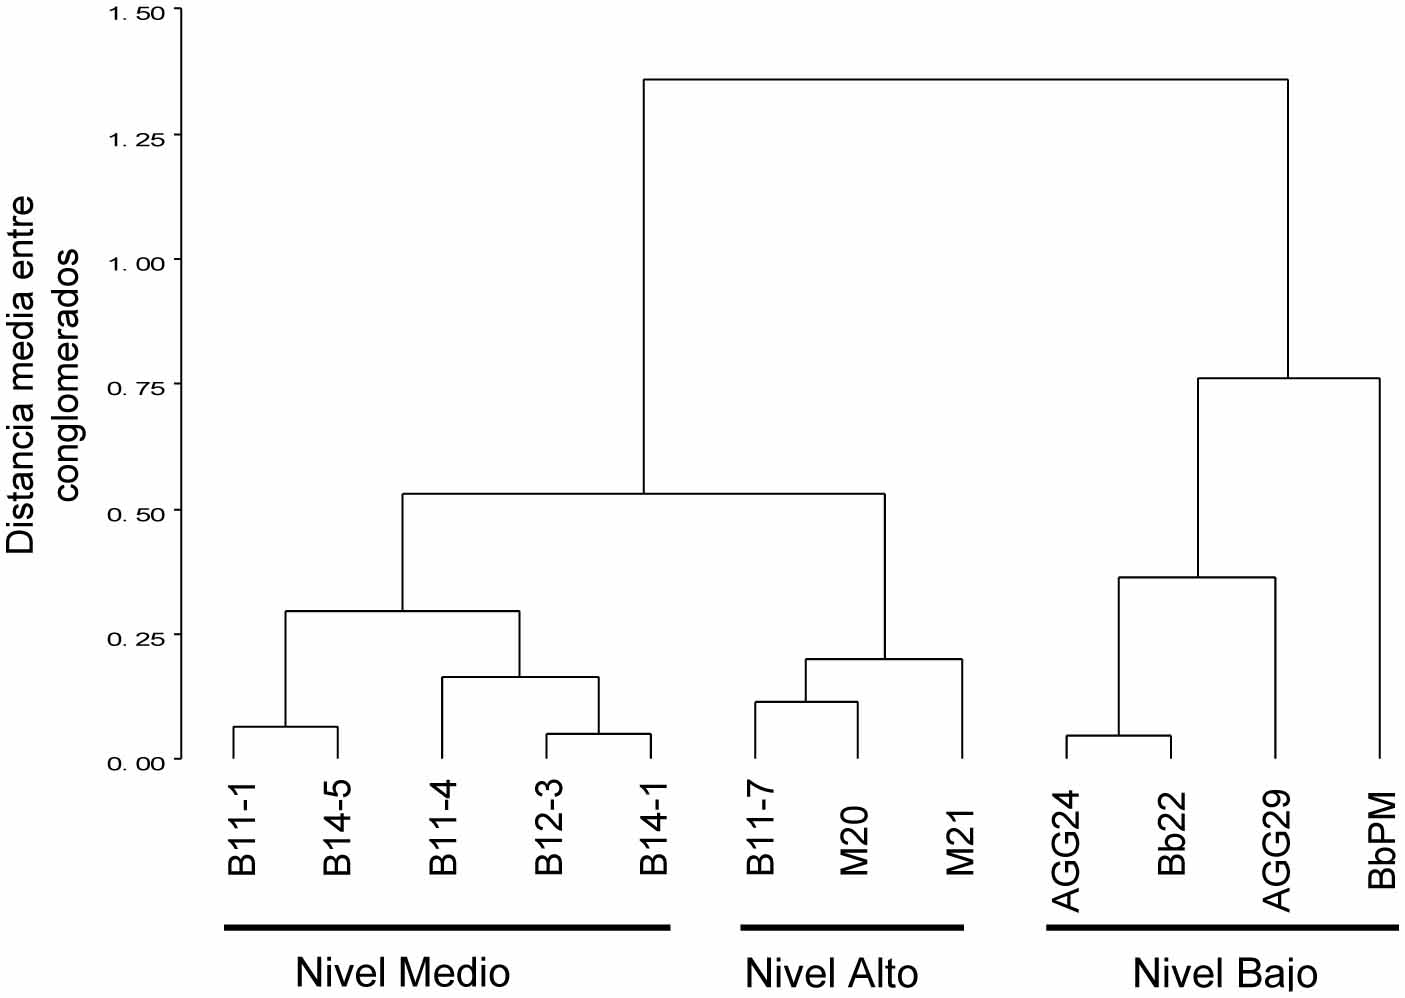
\includegraphics{images/clu.jpg}
\caption{\label{fig:"R2"}}
\end{figure}

A partir del dendrograma se puede apreciar un número apropiado de clúster.

\hypertarget{grafico-de-codo}{%
\subsection{Gráfico de codo}\label{grafico-de-codo}}

Este método considera el porcentaje de varianza explicado en función del número de conglomerados: Se debe elegir un número de clústeres que optimice el modelado, de modo que la mejora sea insignificante si se intenta añadir otro clúster. En otros términos, si se traza el porcentaje de varianza explicado por los clústeres contra el número de clústeres, los primeros clústeres añadirán mucha información (explican mucha varianza), pero en algún momento la ganancia marginal producto de añadir clústeres adicionales caerá, mostrando un ángulo en el gráfico. El número de grupos se elige justo hasta este punto, de ahí el ``criterio del codo''. Este ``codo'' no siempre puede ser identificado inequívocamente. La siguiente imagen nos proporciona una muestra de un gráfico de codo:

\begin{figure}
\centering
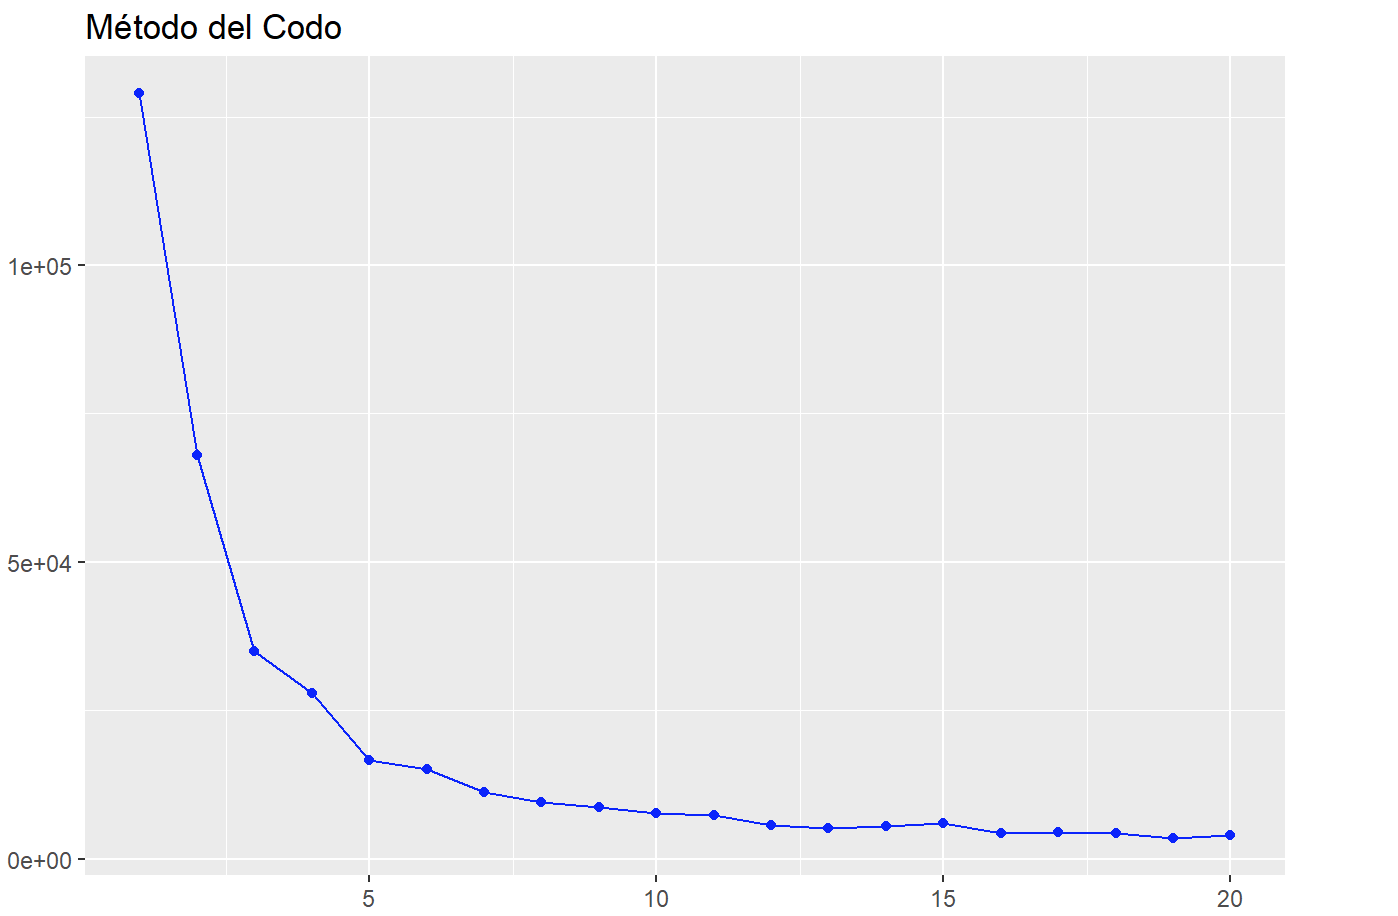
\includegraphics{images/clu1.png}
\caption{\label{fig:"R2"}}
\end{figure}

\hypertarget{analisis-de-cluster-en-r}{%
\section{\texorpdfstring{Análisis de clúster en \emph{R}}{Análisis de clúster en R}}\label{analisis-de-cluster-en-r}}

\hypertarget{metodo-no-jerarquico}{%
\subsection{Método no jerárquico}\label{metodo-no-jerarquico}}

Veremos el método llamado \emph{K-medias} que en resumidas palabras agrupa un número de clústeres pre-definidos a partir de los valores medios de cada clúster. Usaremos el conjunto de datos \emph{iris} con información sobre tres variedades morfológicas de la especie iris, el cual viene por defecto en \emph{R}, también la función \emph{kmeans()} la cual requiere dos parámetros: el conjunto de datos y el número de clústeres a crear.

Lo primero que haremos es calcular un diagrama de codo para poder tener una primera impresión del número de grupos a utilizar, esto lo haremos con el siguiente código:

\begin{figure}
\centering
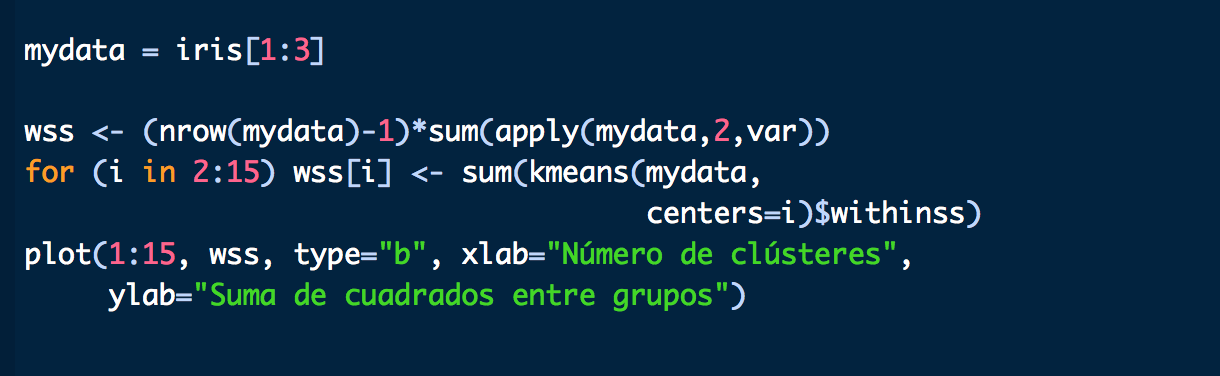
\includegraphics{images/clu7.png}
\caption{\label{fig:"R2"}}
\end{figure}

Obteniendo la siguiente imagen:

\begin{figure}
\centering
\includegraphics{images/clu6.png}
\caption{\label{fig:"R2"}}
\end{figure}

A partir de este gráfico podemos intuir que el número de clústeres adecuados es 3, luego para construir los grupos usaremos el siguiente código:

\begin{figure}
\centering
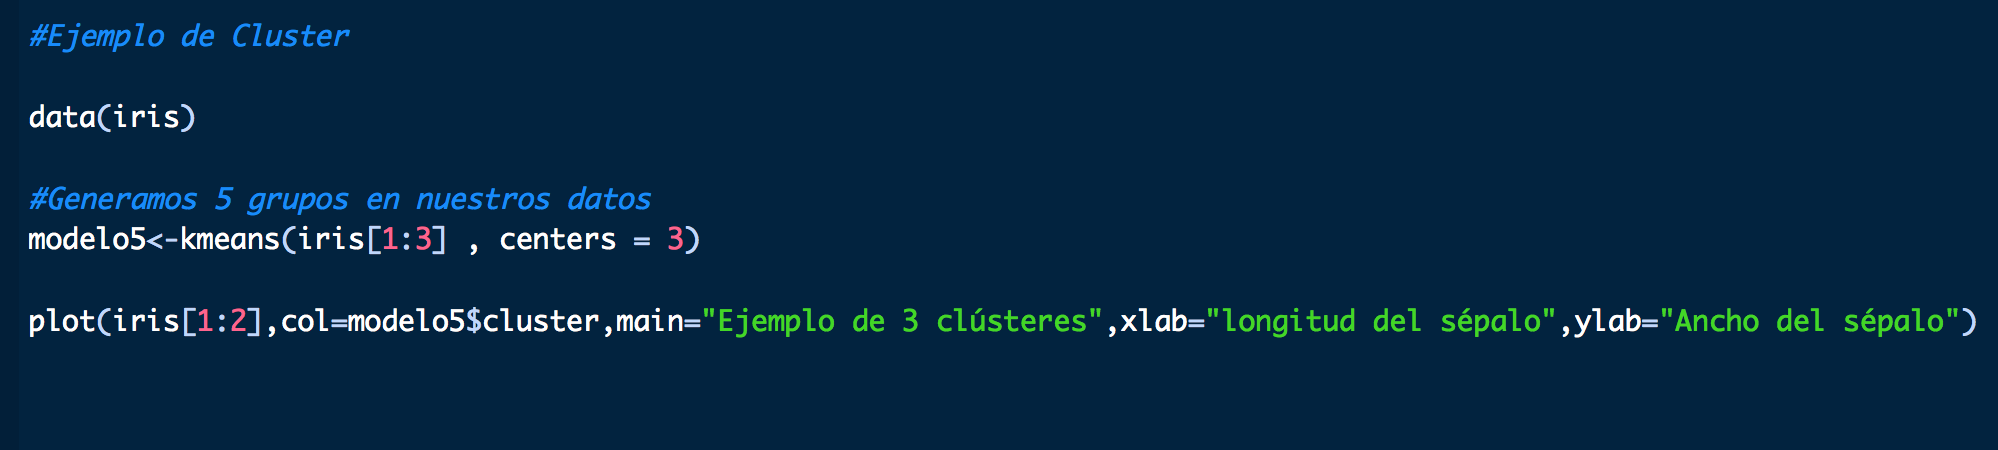
\includegraphics{images/clu2.png}
\caption{\label{fig:"R2"}}
\end{figure}

Para tener una visión gráfica de los clústeres hacemos proyecciones en pares de variables, obteniendo el siguiente gráfico:

\begin{figure}
\centering
\includegraphics{images/clu4.png}
\caption{\label{fig:"R2"}}
\end{figure}

\hypertarget{metodo-jerarquico}{%
\subsection{Método jerárquico}\label{metodo-jerarquico}}

Para construir los grupos, primero debemos crear las distancias entre observaciones, esto lo haremos con la función \emph{dist()}. Esta función tiene como parámetros el conjunto de datos y la manera en cómo se medirán los datos, en nuestro caso con la distancia euclídea. Luego con la función \emph{hclust()} creamos el proceso de agrupación entre individuos, ésta función necesita dos parámetros: las distancias calculadas y el método de agrupación entre los individuos. En nuestro caso usaremos el método ``\emph{complete}''. A continuación realizaremos el gráfico de dendrograma. Veamos esto en el siguiente código:

\begin{figure}
\centering
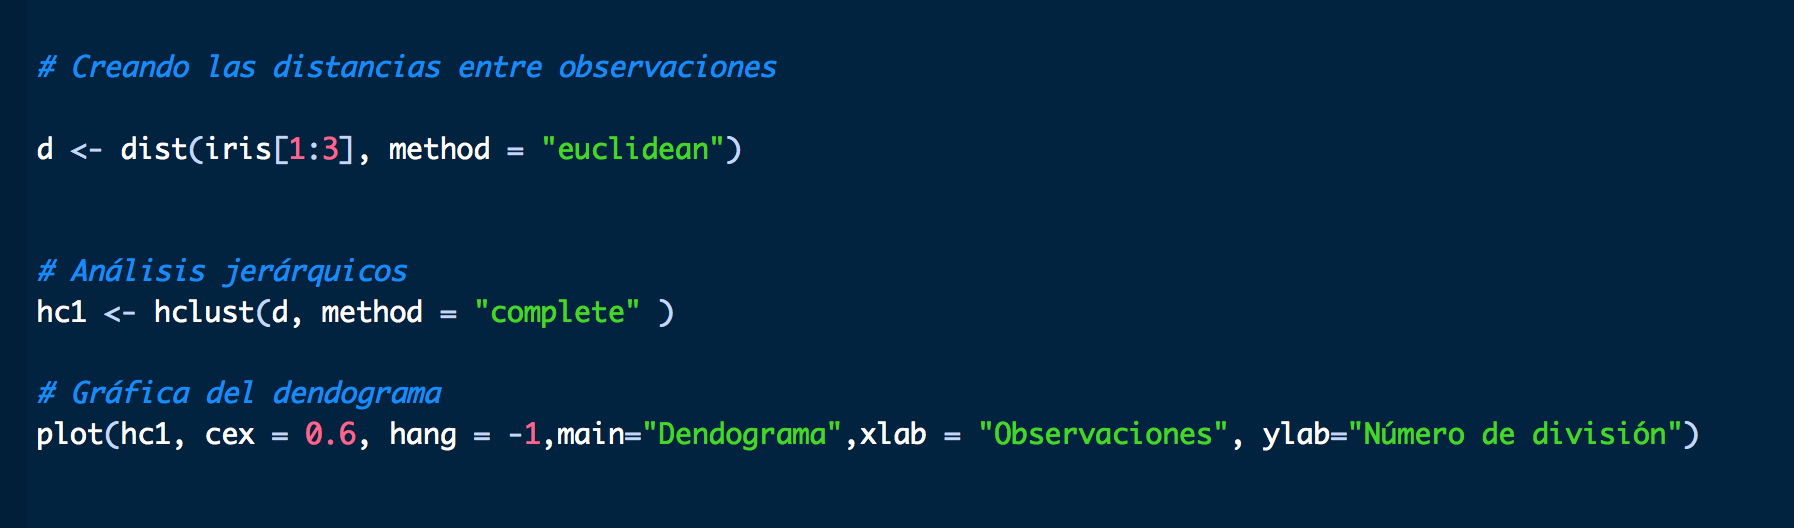
\includegraphics{images/clu9.png}
\caption{\label{fig:"R2"}}
\end{figure}

\begin{figure}
\centering
\includegraphics{images/clu8.png}
\caption{\label{fig:"R2"}}
\end{figure}

Con este dendrograma podemos apreciar una posible separación de la variable de entre 3 o 4 grupos. Para obtener estos grupos, usaremos la función \emph{cutree()} la cual recibe como parámetros el modelo y el número de grupos a escoger, a continuación se muestra este procedimiento:

\begin{figure}
\centering
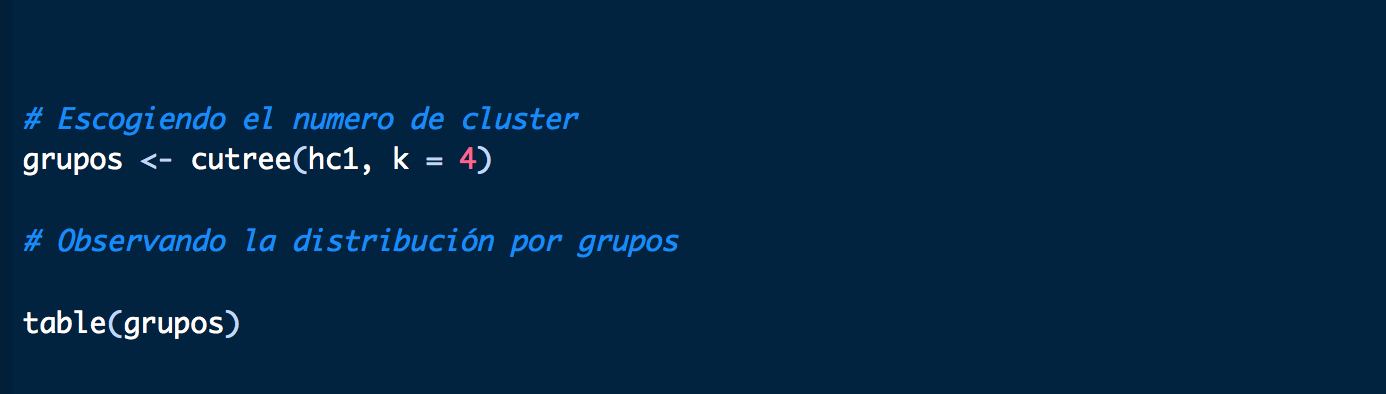
\includegraphics{images/clu10.png}
\caption{\label{fig:"R2"}}
\end{figure}

\hypertarget{analisis-de-cluster-en-python}{%
\section{\texorpdfstring{Análisis de clúster en \emph{Python}}{Análisis de clúster en Python}}\label{analisis-de-cluster-en-python}}

\hypertarget{metodo-no-jerarquico-1}{%
\subsection{Método no jerárquico}\label{metodo-no-jerarquico-1}}

Realizaremos la construcción de los grupos usando el método \emph{kmeans} con el mismo conjunto datos. No describiremos en detalle las librerías a utilizar, solo describiremos su uso general, utilizando la librería \emph{sklearn} para crear el modelo y \emph{seaborn}, \emph{matplotlib} y \emph{mpl\_toolkits} para la parte gráfica.

\begin{figure}
\centering
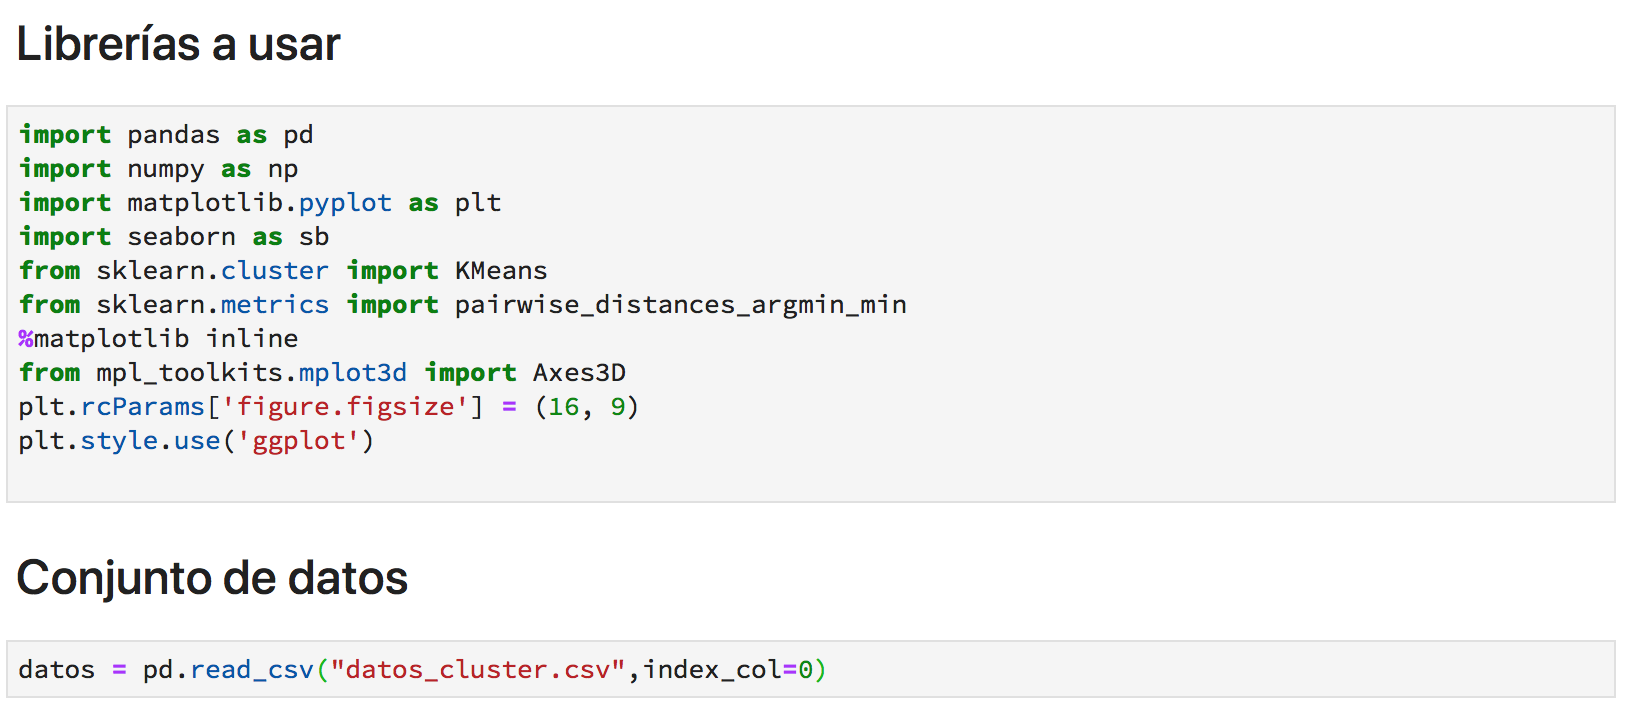
\includegraphics{images/clu11.png}
\caption{\label{fig:"R2"}}
\end{figure}

Ahora construiremos el gráfico de codos para poder determinar el número apropiado de clústeres. Usaremos la función \emph{Kmeans} de la librería \emph{sklearn} para construir los modelos por número de clústeres. Seguidamente se muestra el siguiente código para este propósito.

\begin{figure}
\centering
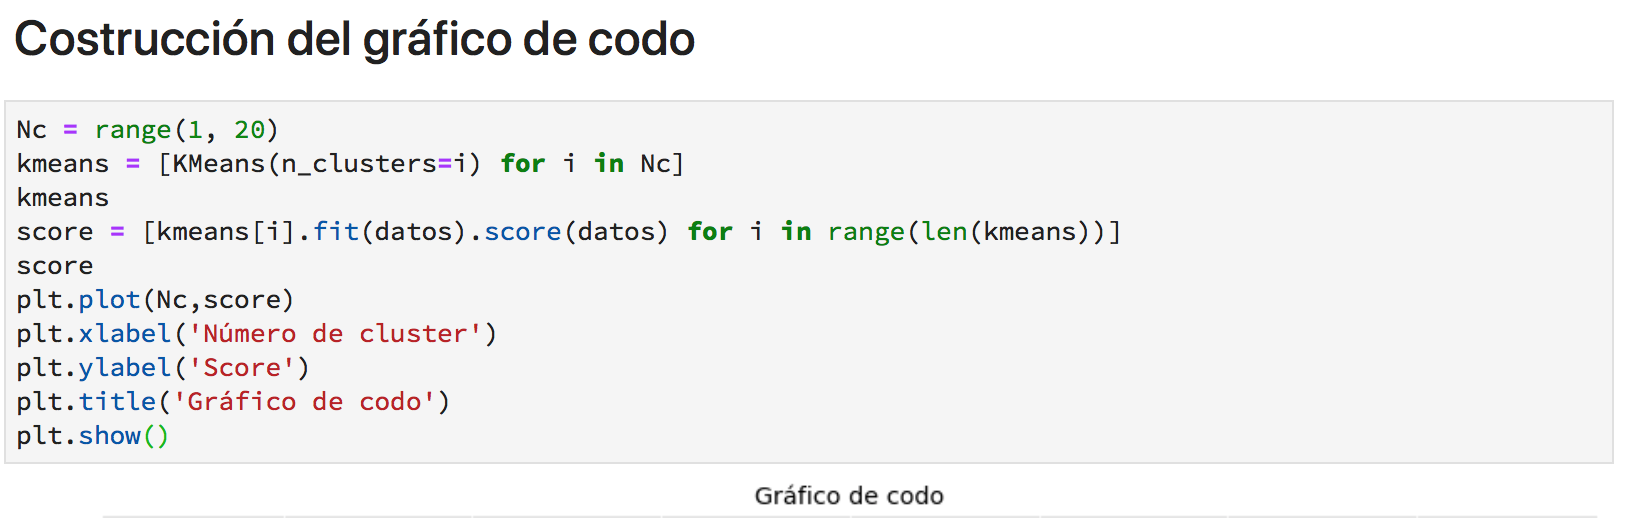
\includegraphics{images/clu12.png}
\caption{\label{fig:"R2"}}
\end{figure}

Obteniendo el siguiente resultado:

\begin{figure}
\centering
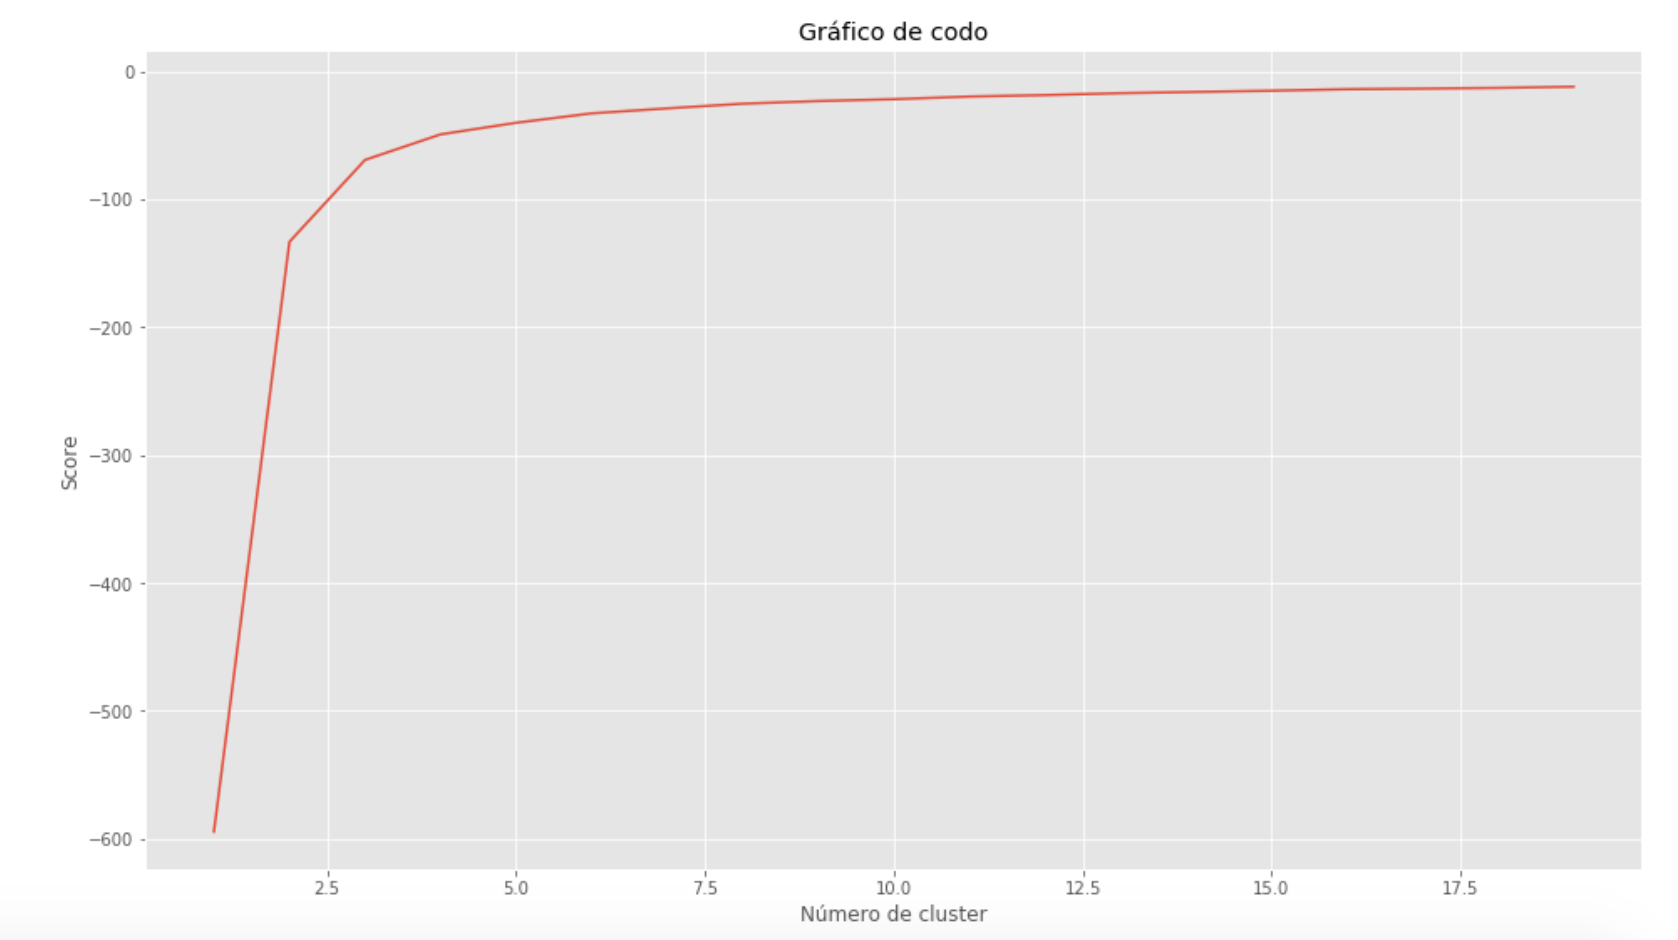
\includegraphics{images/clu13.png}
\caption{\label{fig:"R2"}}
\end{figure}

A partir de este gráfico creamos unos número de tres grupos, con la función \emph{kmean().} Con \emph{.predicts()} identificamos el grupo al cual pertenece cada observación.

\begin{figure}
\centering
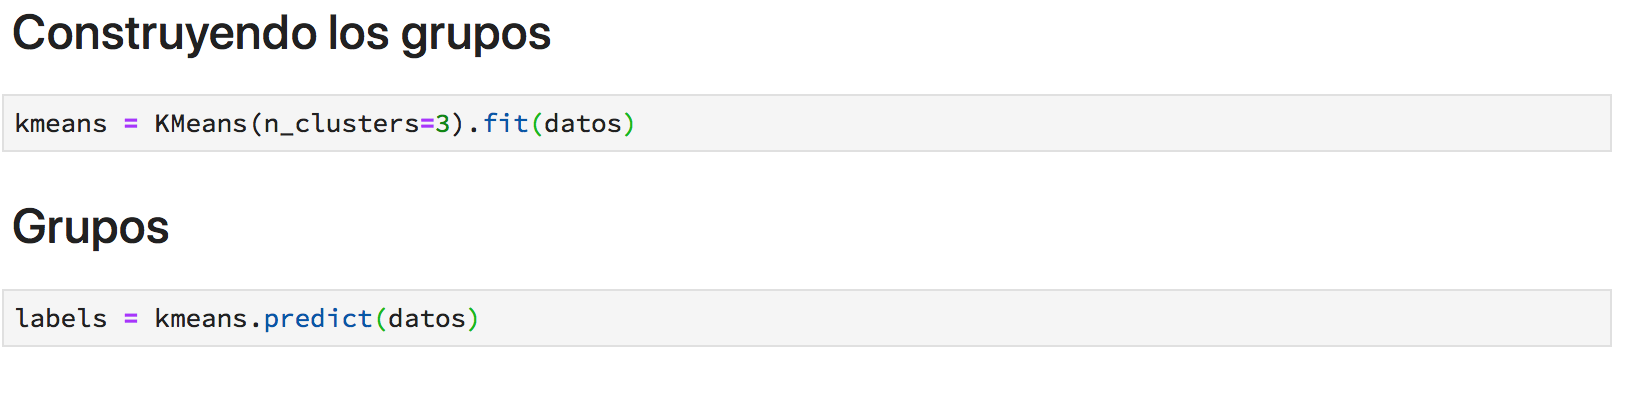
\includegraphics{images/clu14.png}
\caption{\label{fig:"R2"}}
\end{figure}

\hypertarget{metodo-jerarquico-1}{%
\subsection{Método jerárquico}\label{metodo-jerarquico-1}}

Para el cálculo de los grupos usaremos el mismo conjunto de datos, una vez cargados construimos el dendrograma, para lo cual usaremos la función \emph{.dendrogram()} de la librería \emph{scipy}. En este ejemplo usaremos el método de \emph{ward}. A continuación mostramos el código:

\begin{figure}
\centering
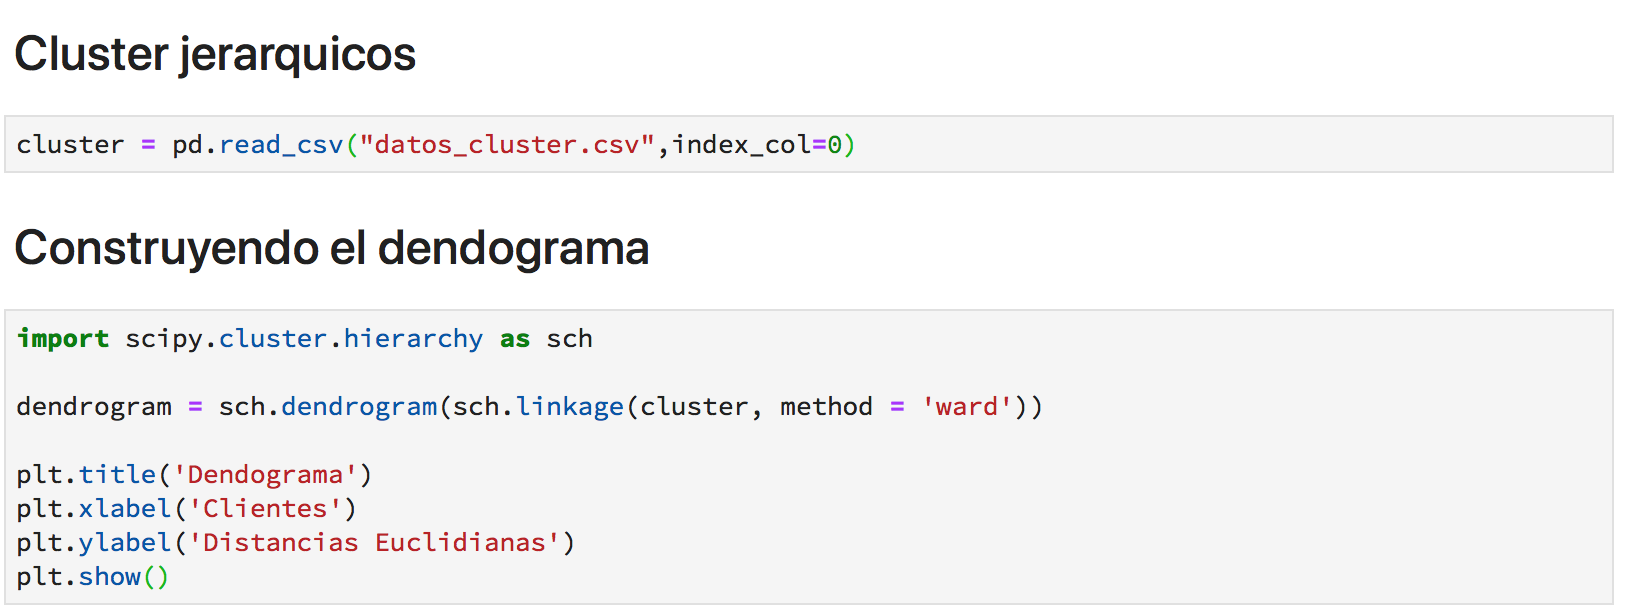
\includegraphics{images/clu15.png}
\caption{\label{fig:"R2"}}
\end{figure}

Este código nos da como resultado :

\begin{figure}
\centering
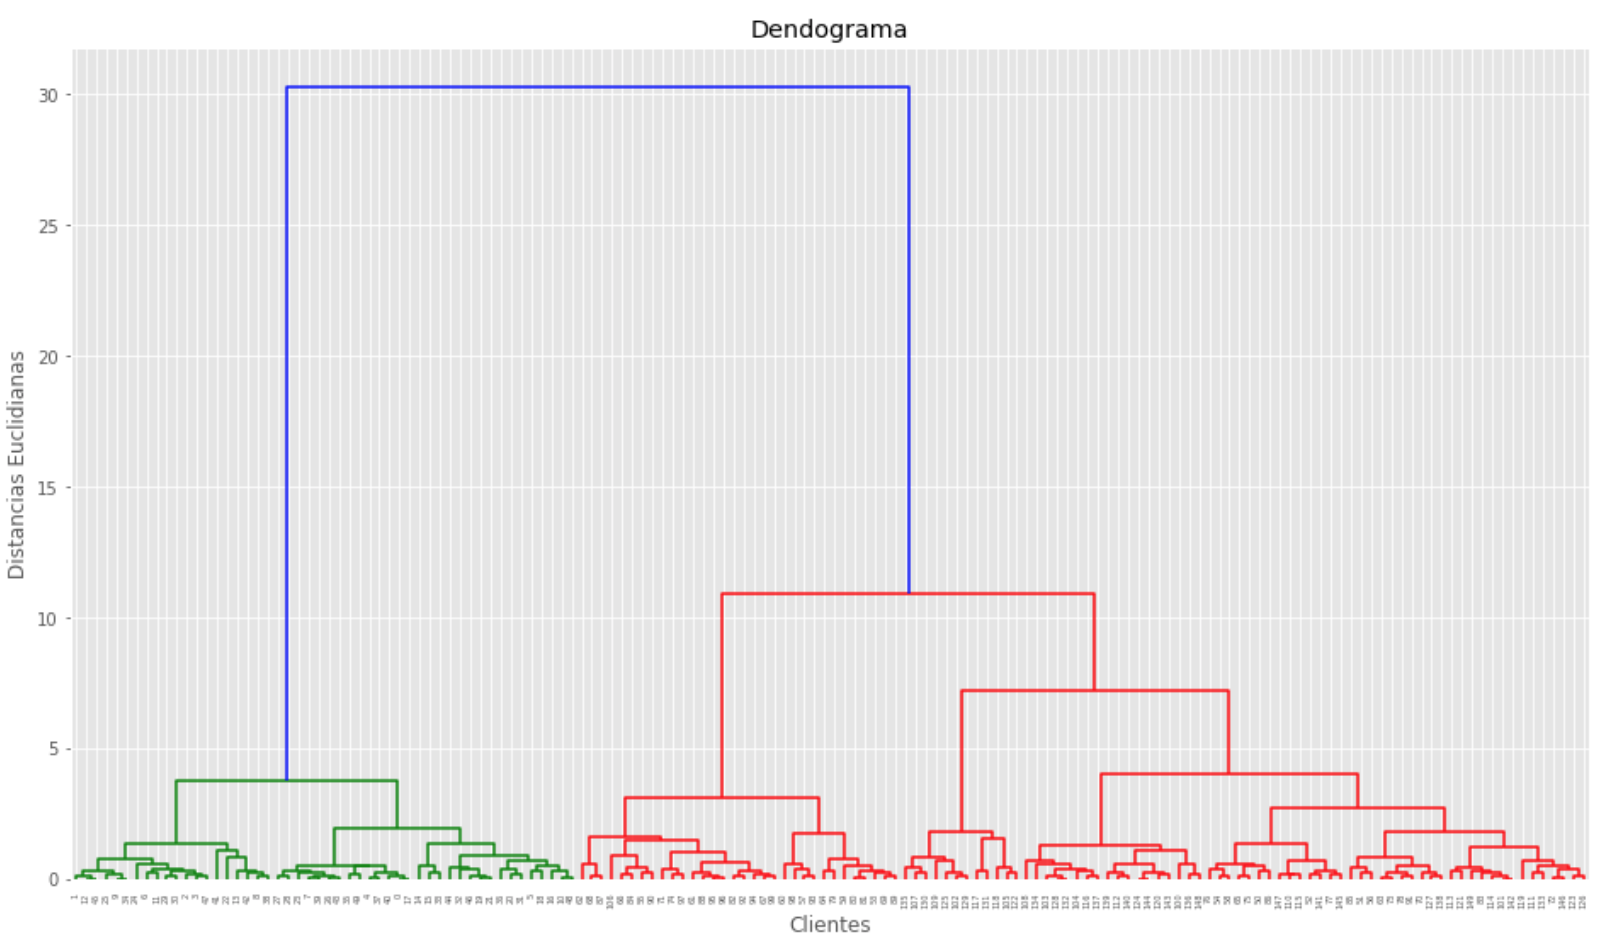
\includegraphics{images/clu16.png}
\caption{\label{fig:"R2"}}
\end{figure}

Al observar el dendrograma observamos la existencia de tres grupos posibles. Para obtenerlos usaremos la función \emph{AgglomerativeClustering()} de la librería \emph{sklear} y finalmente \emph{.fit\_predict()} para obtener los grupos. El procedimiento a seguir se presenta a continuación:

\begin{figure}
\centering
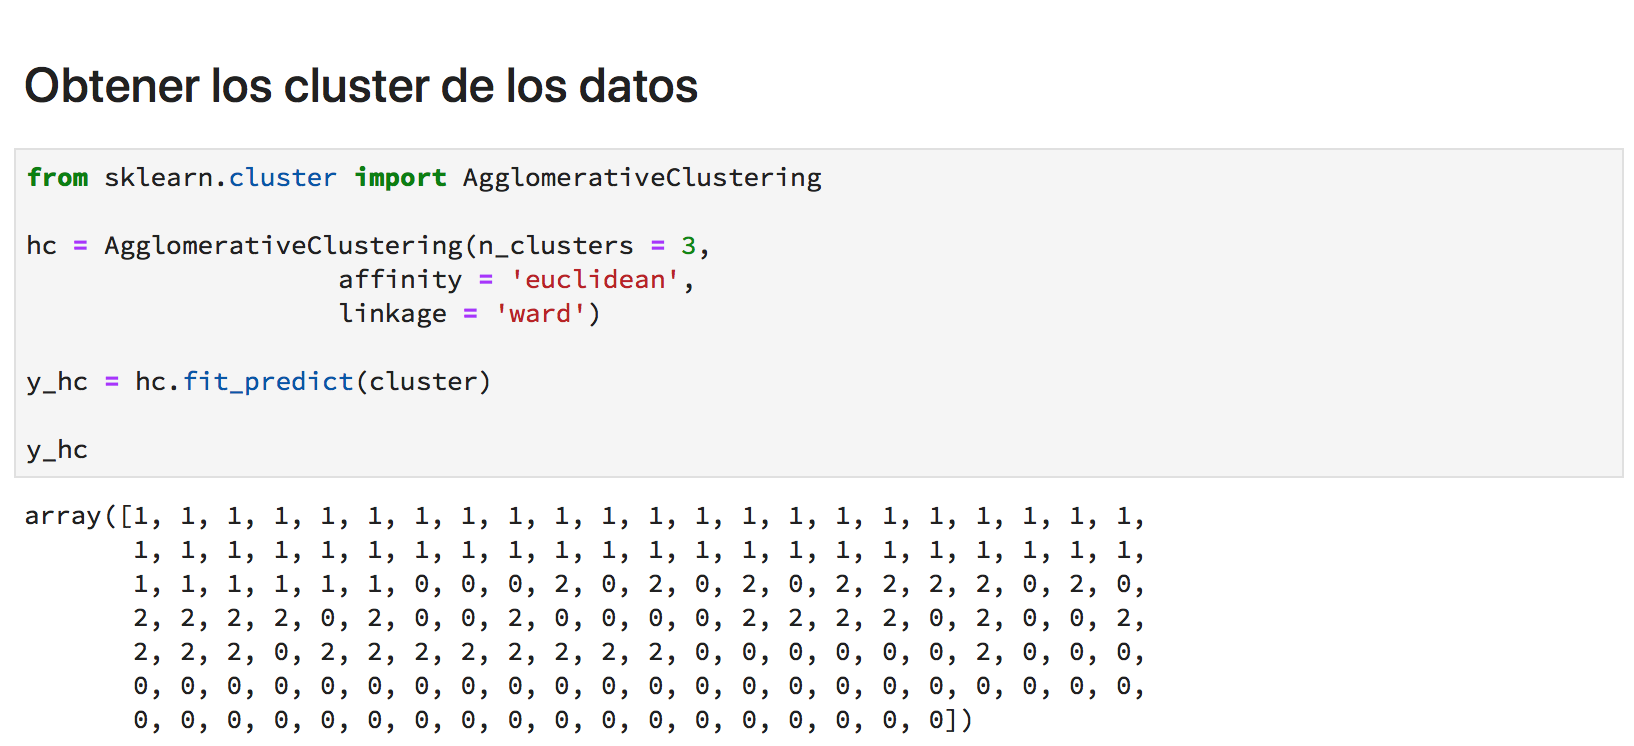
\includegraphics{images/clu17.png}
\caption{\label{fig:"R2"}}
\end{figure}

\hypertarget{analisis-de-componentes-principales}{%
\chapter{Análisis de Componentes Principales}\label{analisis-de-componentes-principales}}

El análisis de componentes principales o PCA por sus siglas en inglés (Principal component analysis), es un método concebido para la reducción de variables que conforman un conjunto de datos. La idea fundamental detrás de la matemática en la que se fundamenta, es crear a través de las variables, un nuevo grupo de variables que tengan muy poca correlación entre sí, de modo que con una cantidad reducida de ellas se pueda explicar la mayor cantidad de varianza del conjunto de datos. Cada variable nueva es llamada componente, en el cual el orden representa la cantidad de varianza explicada, de modo que el nivel de varianza explicada decrece entre mayor sea el orden de la componente a utilizar. Ésta es la clave a la hora de reducir variables, pues en general se escoge un nivel de componentes que explique una cantidad considerable de varianza, por ejemplo, el 80\%.

\hypertarget{correlacion-o-covarianza}{%
\section{Correlación o Covarianza:}\label{correlacion-o-covarianza}}

A la hora de calcular las componentes principales debemos especificar la matriz a utilizar para dichos cálculos, es decir, la matriz de correlación o la matriz de covarianza. El criterio general para dicha escogencia es el siguiente:

\begin{itemize}
\item
  Matriz de correlación: Cuando los datos no son dimensionalmente homogéneos o el orden de magnitud de las variables medidas no es el mismo.
\item
  Matriz de covarianza: Cuando los datos son dimensionalmente homogéneos y presentan valores medios similares.
  En general, se suelen normalizar los datos, es decir, dividir por su varianza y trasladar su valor medio al origen, en este punto se suele usar en la mayoría de los casos la matriz de covarianza.
\end{itemize}

\hypertarget{supuestos-estadisticos}{%
\section{Supuestos estadísticos}\label{supuestos-estadisticos}}

Este análisis exige verificar ciertos supuestos estadísticos:

\begin{itemize}
\item
  Se asume que los datos observados siguen cierta linealidad a través de cierta base de \(\mathbb{R}^n\). Por ejemplo, debemos asegurarnos de que las variables estén lo menos correlacionadas entre sí.
\item
  El \emph{PCA} utiliza los vectores propios de la matriz de covarianzas o correlación y sólo encuentra las direcciones de ejes en el espacio de variables considerando que los datos se distribuyen de manera normal.
\end{itemize}

\hypertarget{pca-en-r}{%
\section{\texorpdfstring{\emph{PCA} en \emph{R}}{PCA en R}}\label{pca-en-r}}

\hypertarget{librerias-y-datos}{%
\subsection{Librerías y datos}\label{librerias-y-datos}}

Usaremos la base de datos \emph{USArrests} la cual viene por defecto en \emph{R} y contiene información acerca de ciertos índices delictivos en EEUU.

Al cargar los datos calcularemos las medias y varianzas de las variables para saber si es necesario normalizar los datos. Para ello empleamos el siguiente código:

\begin{figure}
\centering
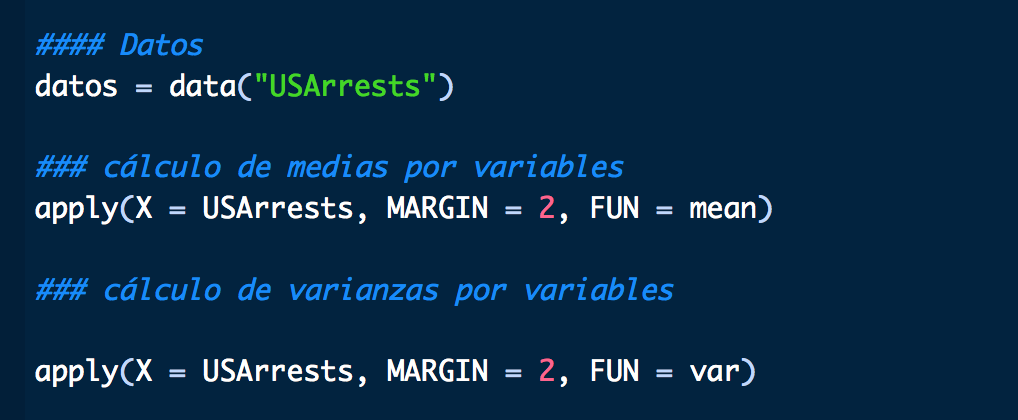
\includegraphics{images/pca1.png}
\caption{\label{fig:"R2"}}
\end{figure}

El primer resultado es la media por variable, observándose considerables diferencias

\begin{figure}
\centering

\includegraphics{images/pca3.png}
\caption{\label{fig:"R2"}}
\end{figure}

De igual manera a continuación podemos observar considerables diferencias en las varianzas entre las variables:

\begin{figure}
\centering
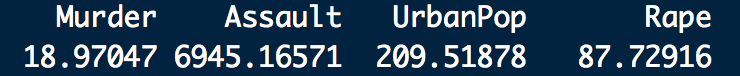
\includegraphics{images/pca2.png}
\caption{\label{fig:"R2"}}
\end{figure}

\hypertarget{calculo-de-componentes}{%
\subsection{Cálculo de componentes}\label{calculo-de-componentes}}

Ahora, con la función \emph{prcomp()} calculamos las componentes principales. Esta función recibe como parámetros los datos y la variable \emph{scale}, la cual de ser \emph{TRUE} normaliza los datos y de ser \emph{FALSE} los deja en su forma original. Una vez hecho lo anterior podemos a través del atributo \emph{rotation} ver los datos en función de las nuevas componentes.

\begin{figure}
\centering
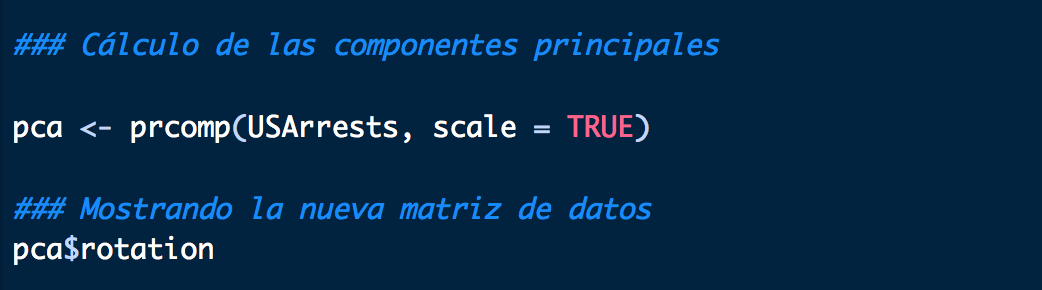
\includegraphics{images/pca4.png}
\caption{\label{fig:"R2"}}
\end{figure}

\begin{figure}
\centering
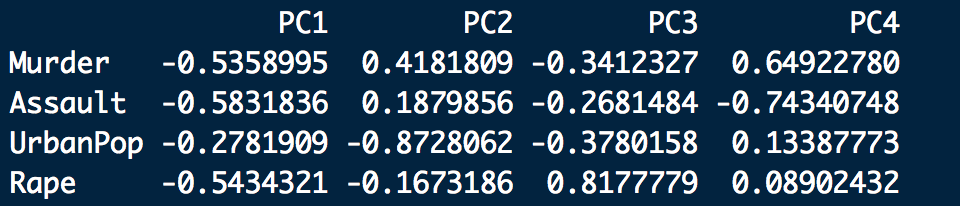
\includegraphics{images/pca5.png}
\caption{\label{fig:"R2"}}
\end{figure}

\hypertarget{funciones-graficas}{%
\subsection{Funciones gráficas}\label{funciones-graficas}}

Ahora para escoger el número de componentes utilizaremos el gráfico de codo. Para ello debemos calcular previamente la varianza por componente. Además, usaremos el paquete \(ggplot\) para obtener una gráfica más elegante. A continuación se muestra este proceso:

\begin{figure}
\centering
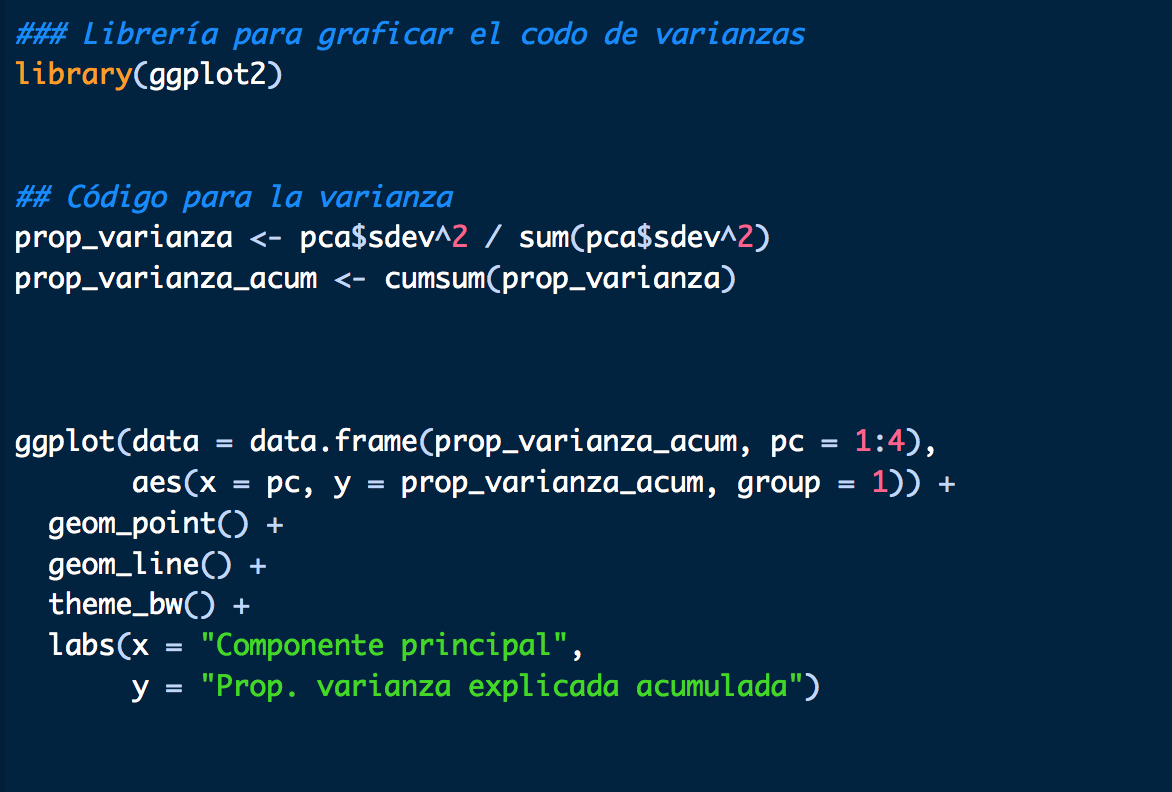
\includegraphics{images/pca6.png}
\caption{\label{fig:"R2"}}
\end{figure}

\begin{figure}
\centering
\includegraphics{images/pca7.png}
\caption{\label{fig:"R2"}}
\end{figure}

Con el gráfico anterior podemos intuir que con tres componentes obtendremos una gran parte de la varianza explicada.

\hypertarget{pca-en-python}{%
\section{\texorpdfstring{\emph{PCA} en \emph{Python}}{PCA en Python}}\label{pca-en-python}}

\hypertarget{librerias-y-datos-1}{%
\subsection{Librerías y datos}\label{librerias-y-datos-1}}

Procederemos a construir el modelo en \emph{Python}, primero cargaremos las librerías y datos a usar, usaremos \emph{sklearn} para constriur el modelo y los mismos datos de la sección anterior

\begin{figure}
\centering
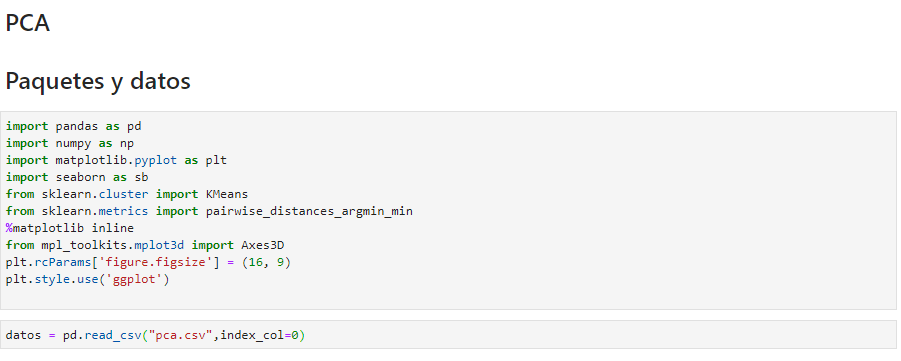
\includegraphics{images/pca8.png}
\caption{\label{fig:"R2"}}
\end{figure}

\hypertarget{calculo-de-componentes-1}{%
\subsection{Cálculo de componentes}\label{calculo-de-componentes-1}}

Procedemos a ver la estructura de los datos, usando las funciones \emph{.mean()} y \emph{.var()} de \emph{Pandas} para calcular la media y varianza de cada variable del conjunto de datos.

\begin{figure}
\centering
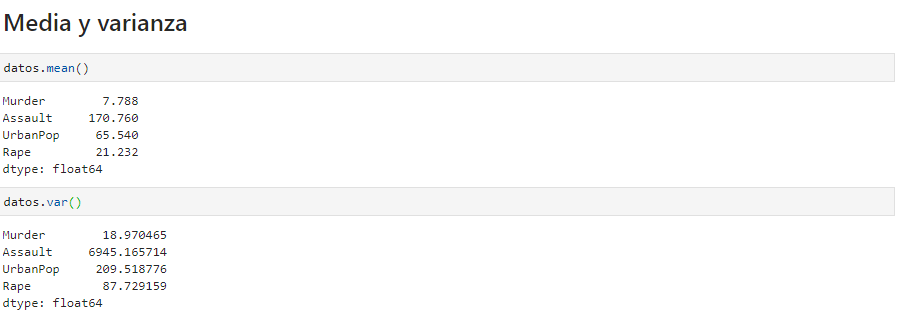
\includegraphics{images/pca9.png}
\caption{\label{fig:"R2"}}
\end{figure}

Observamos que los datos tienen escalas muy diferentes, por lo que procedemos a realizar la normalización de los datos, usando la función \emph{scale()} de \emph{Sklear}. Una vez tenemos los datos con la misma escala, usamos las funciones \emph{PCA()} y \emph{.fit()} para construir el modelo. Finalizamos usando la función \emph{.transform()} para convertir los datos originales a las nuevas componentes calculadas.

\begin{figure}
\centering
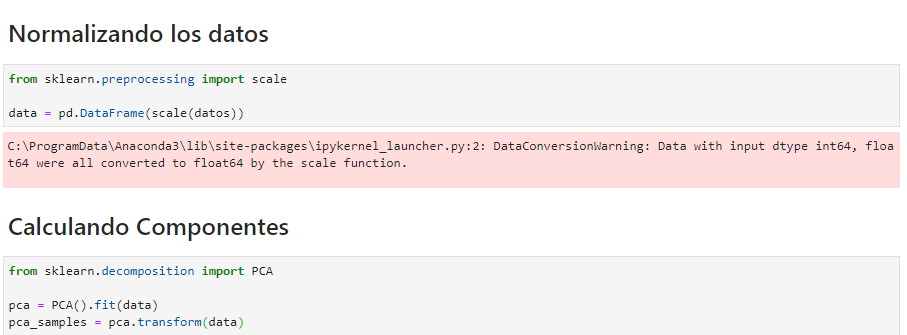
\includegraphics{images/pca10.png}
\caption{\label{fig:"R2"}}
\end{figure}

\hypertarget{funciones-graficas-1}{%
\subsection{Funciones Gráficas}\label{funciones-graficas-1}}

Como este curso no es de programación, anexaremos directamente el siguiente código sin mayores detalles, con el proposito de realizar las gráficas correspondientes del modelo:

\begin{figure}
\centering
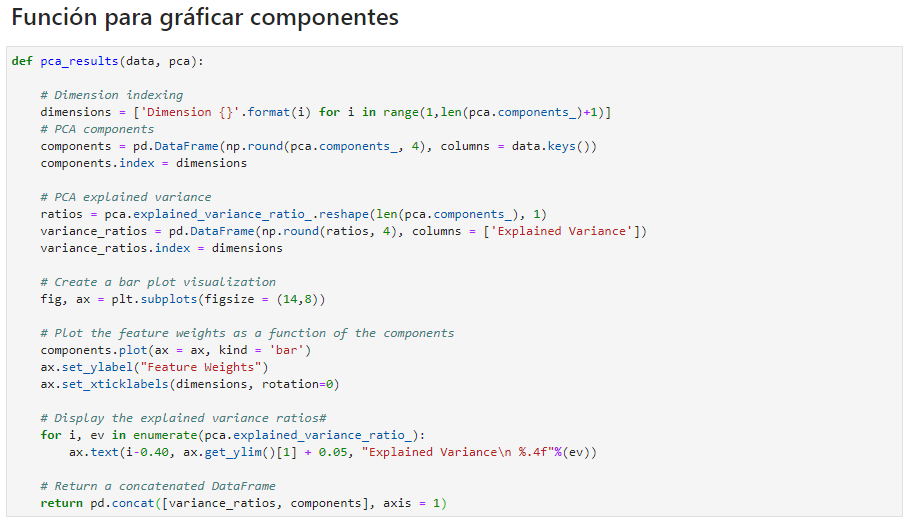
\includegraphics{images/pca11.png}
\caption{\label{fig:"R2"}}
\end{figure}

A continuación anexamos el gráfico de codo:

\begin{figure}
\centering
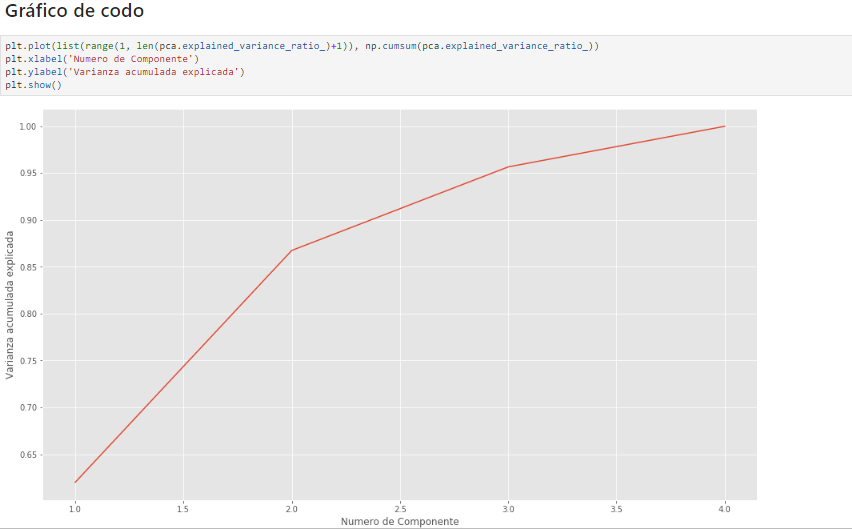
\includegraphics{images/pca13.png}
\caption{\label{fig:"R2"}}
\end{figure}

Con el gráfico de codo podemos apreciar que con \(2\) o \(3\) componentes tenemos una gran cantidad de varianza explicada.

\hypertarget{arboles-de-decision-y-bosques-aleatorios}{%
\chapter{Árboles de decisión y bosques aleatorios}\label{arboles-de-decision-y-bosques-aleatorios}}

\hypertarget{arboles-de-decision}{%
\section{Árboles de decisión}\label{arboles-de-decision}}

Los árboles de decisión son una herramienta muy útil a la hora de elegir entre varias
alternativas, cuando estas son escalonadas, es decir, que los resultados (positivos
o negativos) dependen de una decisión tomada anteriormente. Independientemente del área en que sean utilizados, los árboles de decisión facilitan la visualización y el análisis de las probabilidades de los resultados entre diferentes opciones, mejorando la capacidad de las empresas e individuos para realizar una mejor elección.

Un árbol de decisión es, para quien va a tomar la decisión, un modelo esquemático de las alternativas disponibles y de las posibles consecuencias de cada una. El nombre de la herramienta proviene de la forma que adopta el modelo, el cual semeja un árbol. El modelo está conformado por múltiples nodos cuadrados que representan puntos de decisión. De estos puntos surgen ramas (que deben leerse de izquierda a derecha), las cuales representan las distintas alternativas. Las ramas que provienen de los nodos circulares o causales representan los eventos. A continuación presentamos un ejemplo gráfico de un árbol de decisión:

\begin{figure}
\centering
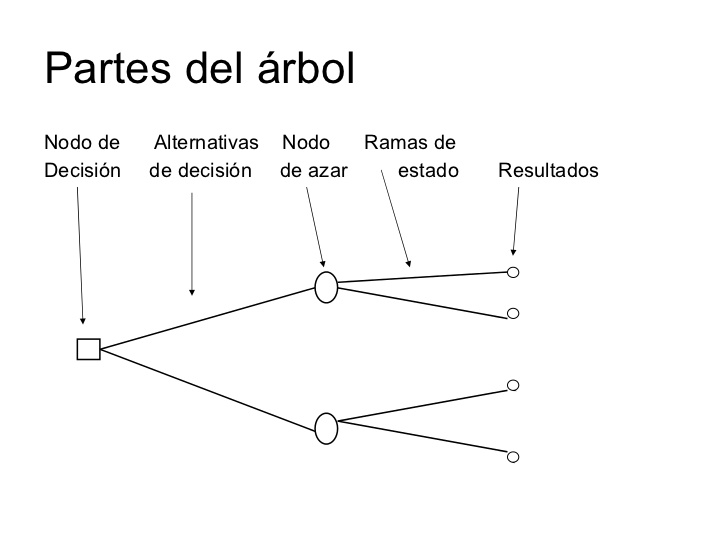
\includegraphics{images/arb1.jpg}
\caption{\label{fig:"R2"}}
\end{figure}

\hypertarget{arboles-de-decision-en-r}{%
\subsection{\texorpdfstring{Árboles de decisión en \emph{R}}{Árboles de decisión en R}}\label{arboles-de-decision-en-r}}

Para realizar la construcción de árboles de decisión usaremos la librería \emph{C50}, junto con la función \emph{C5.0()} con una sintaxis similar a la de la regresión lineal, es decir, ingresamos la variable a predecir seguida de las variables independientes. El segundo parámetro son los datos que se usarán. A continuación se muestra este proceso:

\begin{figure}
\centering
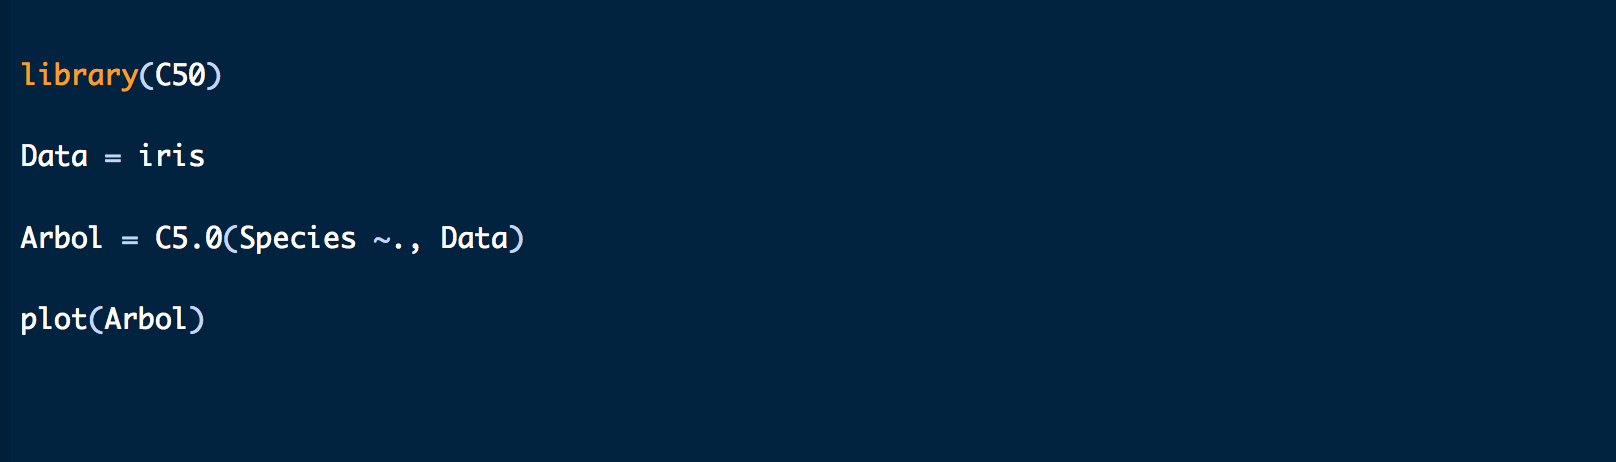
\includegraphics{images/arb3.png}
\caption{\label{fig:"R2"}}
\end{figure}

Al usar la función \emph{plot()} obtenemos la gráfica del árbol de decisión calculado.

\begin{figure}
\centering
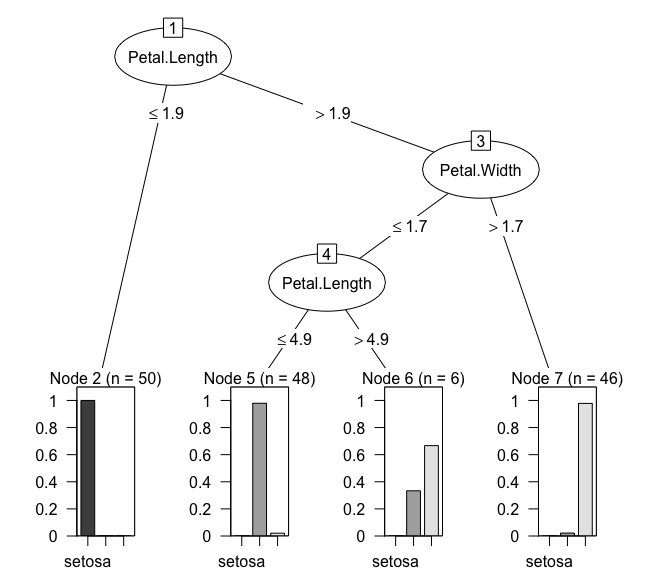
\includegraphics{images/Arb2.png}
\caption{\label{fig:"R2"}}
\end{figure}

Para hacer predicciones, usaremos la función \emph{predict()} la cual necesita como argumentos el nombre del modelo y los datos a predecir.

Para ello construimos unos posibles datos para predecir los resultsdos del modelo \emph{``Arbol''}, como se muestra en el siguiente ejemplo:

\begin{figure}
\centering
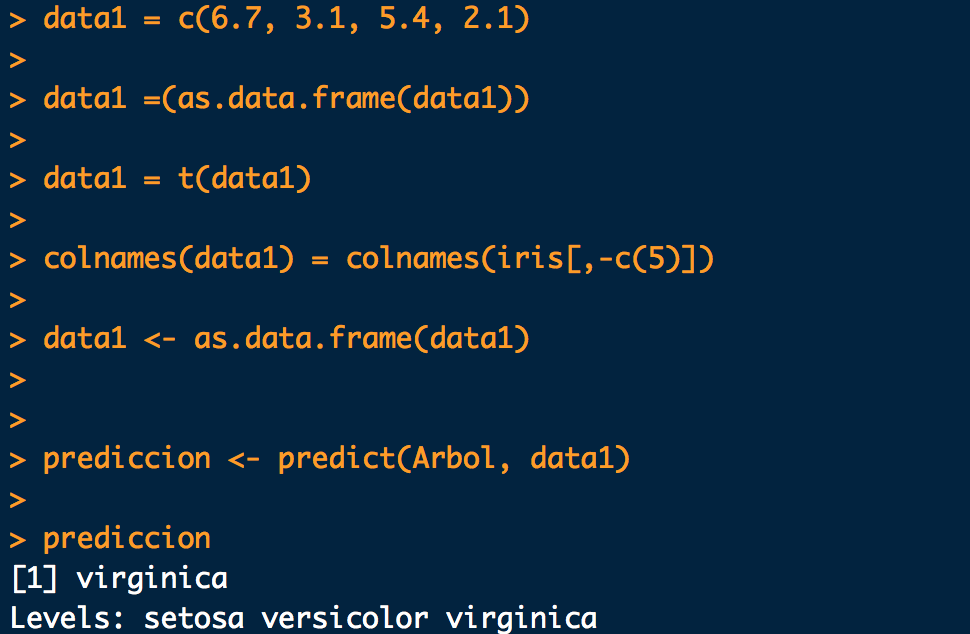
\includegraphics{images/arb4.png}
\caption{\label{fig:"R2"}}
\end{figure}

\hypertarget{arboles-de-decision-en-python}{%
\subsection{\texorpdfstring{Árboles de decisión en \emph{Python}}{Árboles de decisión en Python}}\label{arboles-de-decision-en-python}}

Usaremos la librería \emph{sklearn} y los datos \emph{iris}. Se debe separar la variable a predecir de la variable independiente antes de realizar la construcción del modelo.

\begin{figure}
\centering
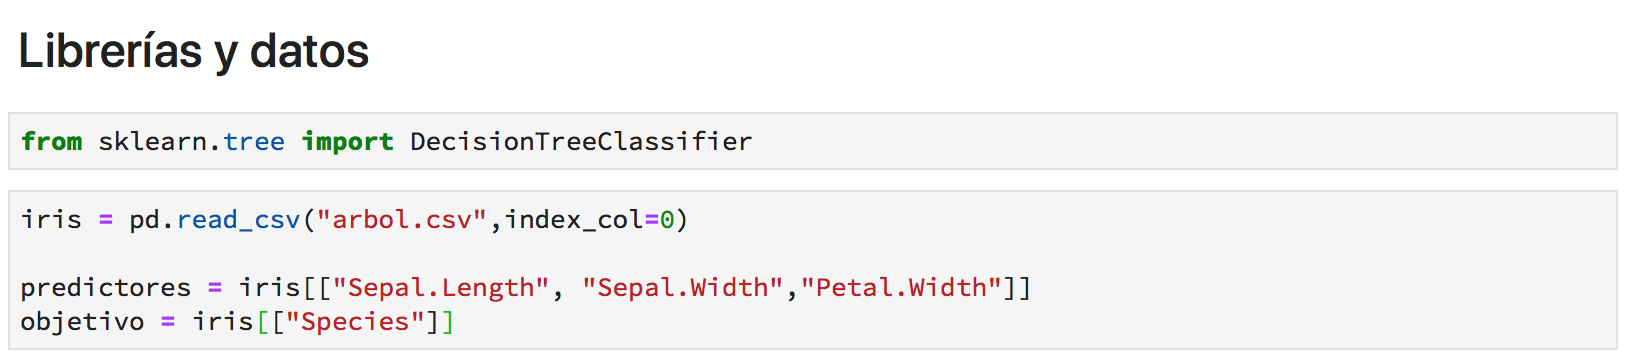
\includegraphics{images/arb5.png}
\caption{\label{fig:"R2"}}
\end{figure}

Construimos el modelo usando usando la función \emph{DecisionTreeClassifier()} y luego lo entrenamos usando usando la función \emph{.fit()} agregando como parámetros la variable independiente y las variables independientes.

\begin{figure}
\centering
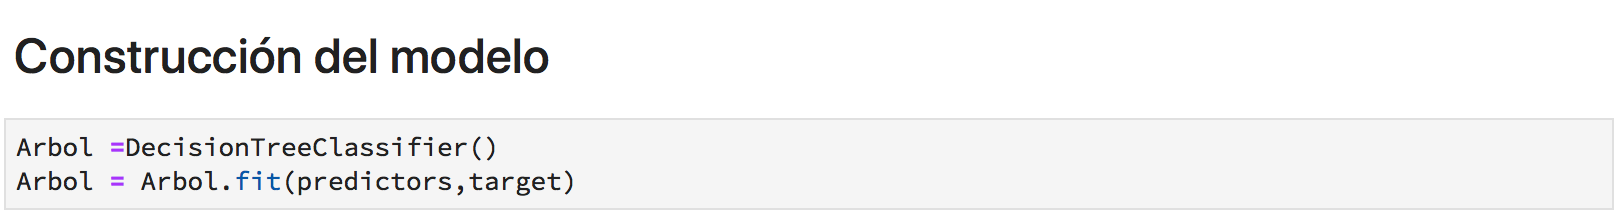
\includegraphics{images/arb6.png}
\caption{\label{fig:"R2"}}
\end{figure}

Para realizar predicciones usamos la función \emph{.predict()}

\begin{figure}
\centering
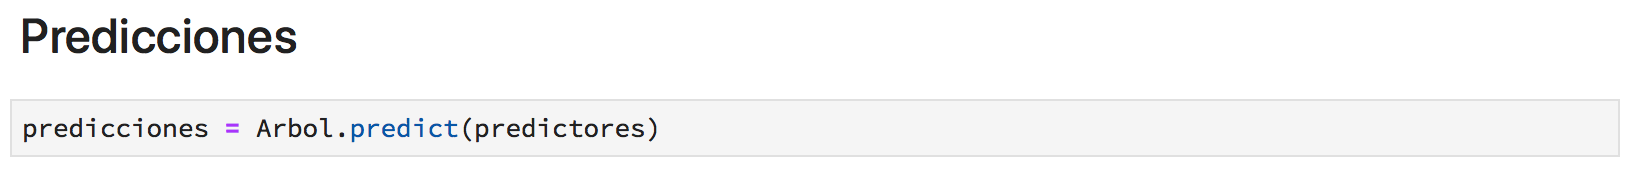
\includegraphics{images/arb7.png}
\caption{\label{fig:"R2"}}
\end{figure}

\hypertarget{bosques-aleatorios}{%
\section{Bosques aleatorios}\label{bosques-aleatorios}}

Bosques aleatorios es una herramienta que combina árboles de decisión, seleccionando de manera aleatoria una cantidad de variables con las cuales se construye cada uno de los árboles individuales, y se realizan predicciones con estas variables que posteriormente serán ponderadas a través del cálculo de la clase más votada de los árboles que se generaron, para finalmente hacer la predicción. El método promedia una colección de árboles no correlacionados, o decorrrelacionados, y dónde cada árbol depende de los valores de un vector aleatorio de la muestra de manera independiente y con la misma distribución de todos los árboles en el bosque. La generalización del error para los bosques converge a un límite en cuanto el número de árboles en el bosque sea grande. El error de generalización de un bosque de árboles de clasificación depende de la fuerza de los árboles individuales en el bosque y la correlación entre ellos.

\hypertarget{bosques-aleatorios-en-r}{%
\section{\texorpdfstring{Bosques aleatorios en \emph{R}}{Bosques aleatorios en R}}\label{bosques-aleatorios-en-r}}

Para realizar bosques aleatorios en \emph{R} usaremos la librería \emph{randomForest} la cual facilita la sintaxis necesaria para construir el modelo. Los datos corresponden a la base de datos \emph{iris} y se debe separar la variable independiente de las dependientes para luego usar la función \emph{randomForest()} para construir el modelo. Ésta función necesita como parámetros las variables independientes y la variable dependiente junto al número de árboles a promediar. Anexamos el código para este proceso:

\begin{figure}
\centering
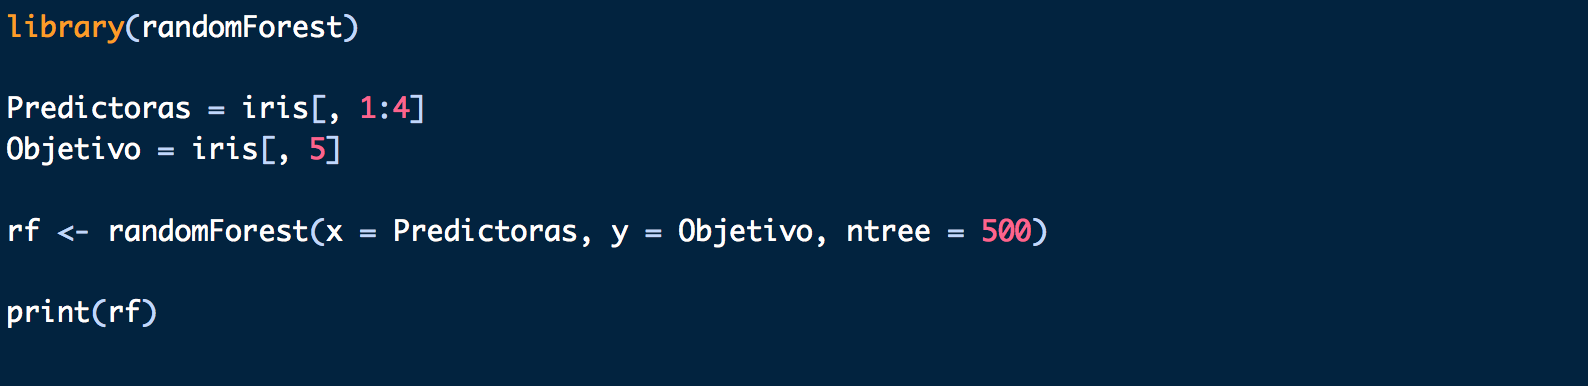
\includegraphics{images/arb8.png}
\caption{\label{fig:"R2"}}
\end{figure}

Al realizar el \emph{print} del modelo obtenemos:

\begin{figure}
\centering
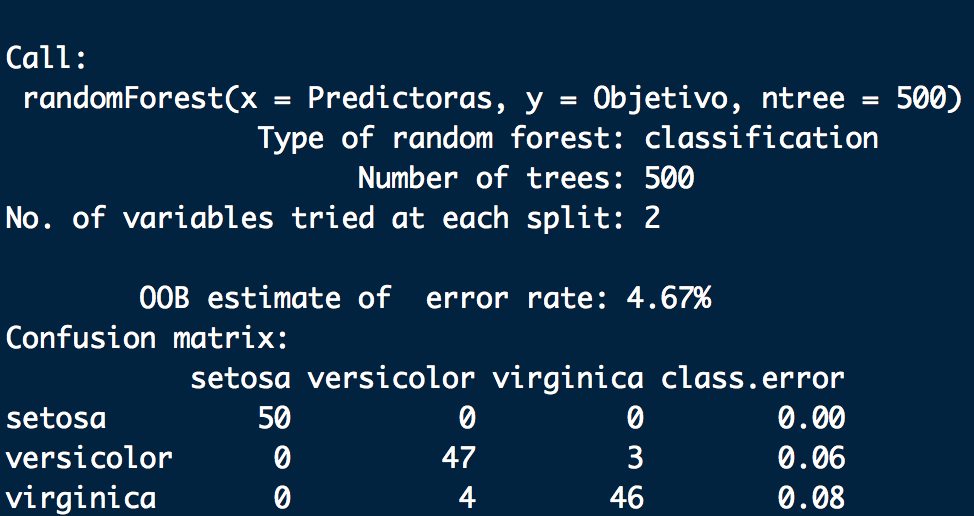
\includegraphics{images/arb9.png}
\caption{\label{fig:"R2"}}
\end{figure}

Aquí obtenemos la información sobre cómo se construyó el modelo y la clasificación de los datos. En el ejemplo notamos que el modelo es muy preciso. Las predicciones la hacemos de la manera habitual, usando la función \emph{predict()} incorporando los parámetros correspondientes al nombre del modelo y al conjunto de nuevos datos:

\begin{figure}
\centering
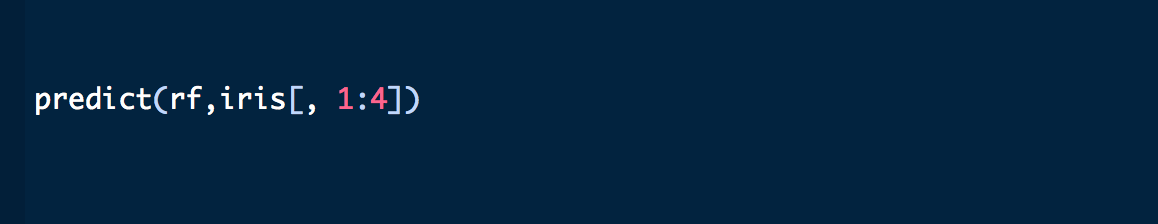
\includegraphics{images/arb10.png}
\caption{\label{fig:"R2"}}
\end{figure}

\hypertarget{bosques-aleatorios-en-python}{%
\section{\texorpdfstring{Bosques aleatorios en \emph{Python}}{Bosques aleatorios en Python}}\label{bosques-aleatorios-en-python}}

Usaremos de igual manera la librería \emph{sklearn}, a modo de conocimiento cargaremos los datos \emph{iris} desde \emph{sklearçn}, pero tendremos que hacerles unas modificaciones previas, de la siguiente forma:
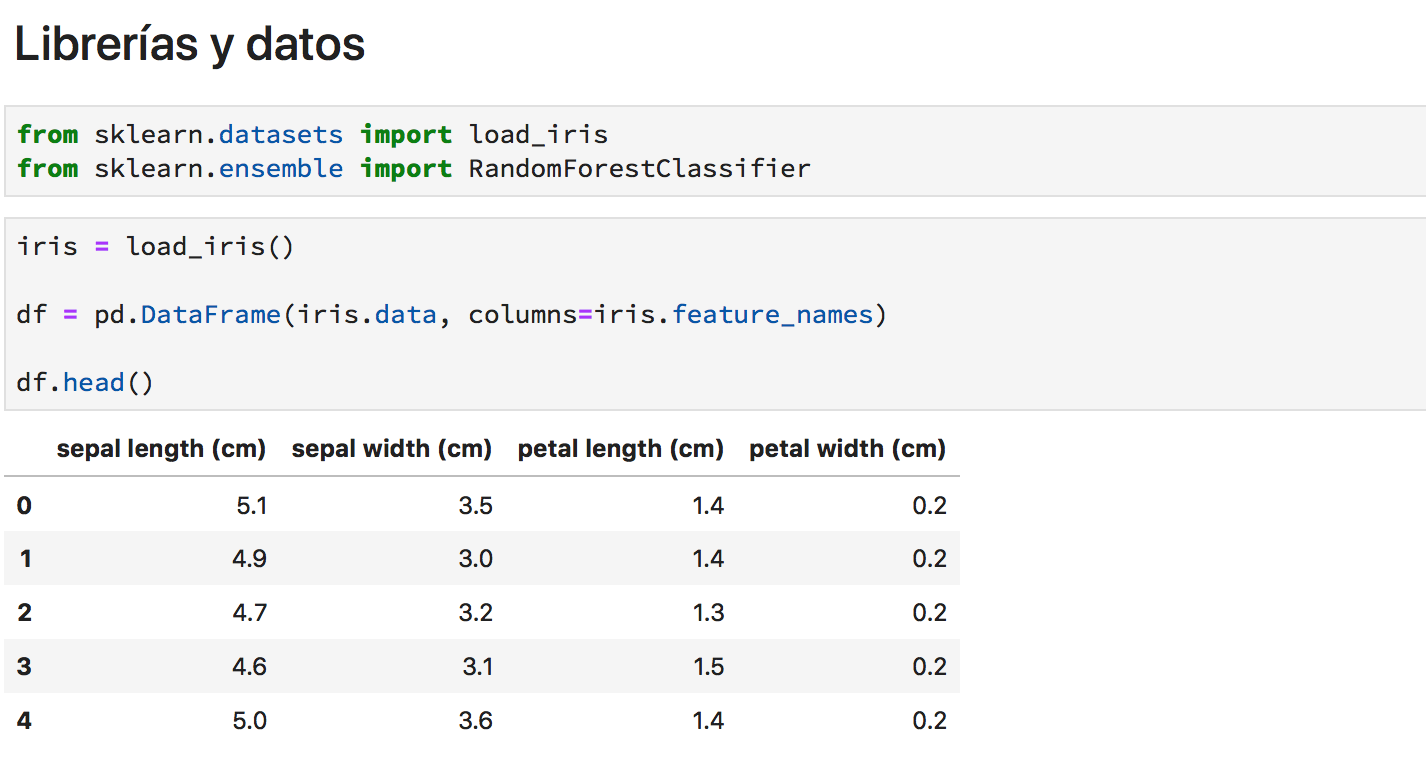
\includegraphics{images/bos5.png}

Debemos separar las variables independientes, en otra variable que llamaremos \emph{predictores}. Como los datos carecen de la variable \emph{species} la agregaremos de la siguiente forma:

\begin{figure}
\centering
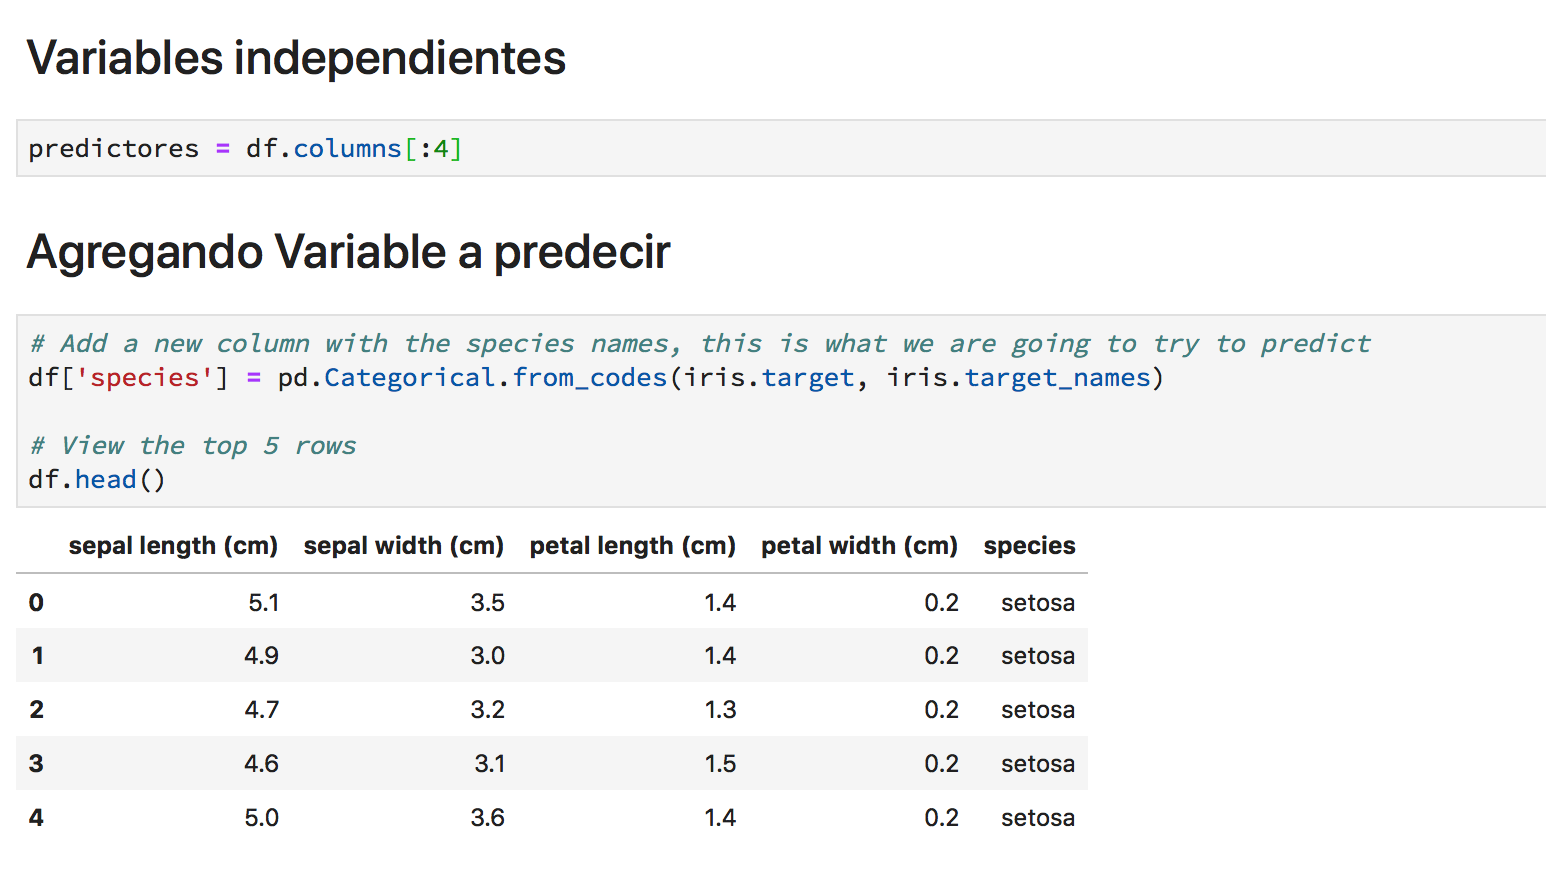
\includegraphics{images/bos1.png}
\caption{\label{fig:"R2"}}
\end{figure}

Antes de construir el modelo, aseguramos que la variable sea del tipo numérico con la función \emph{factorize}:

\begin{figure}
\centering
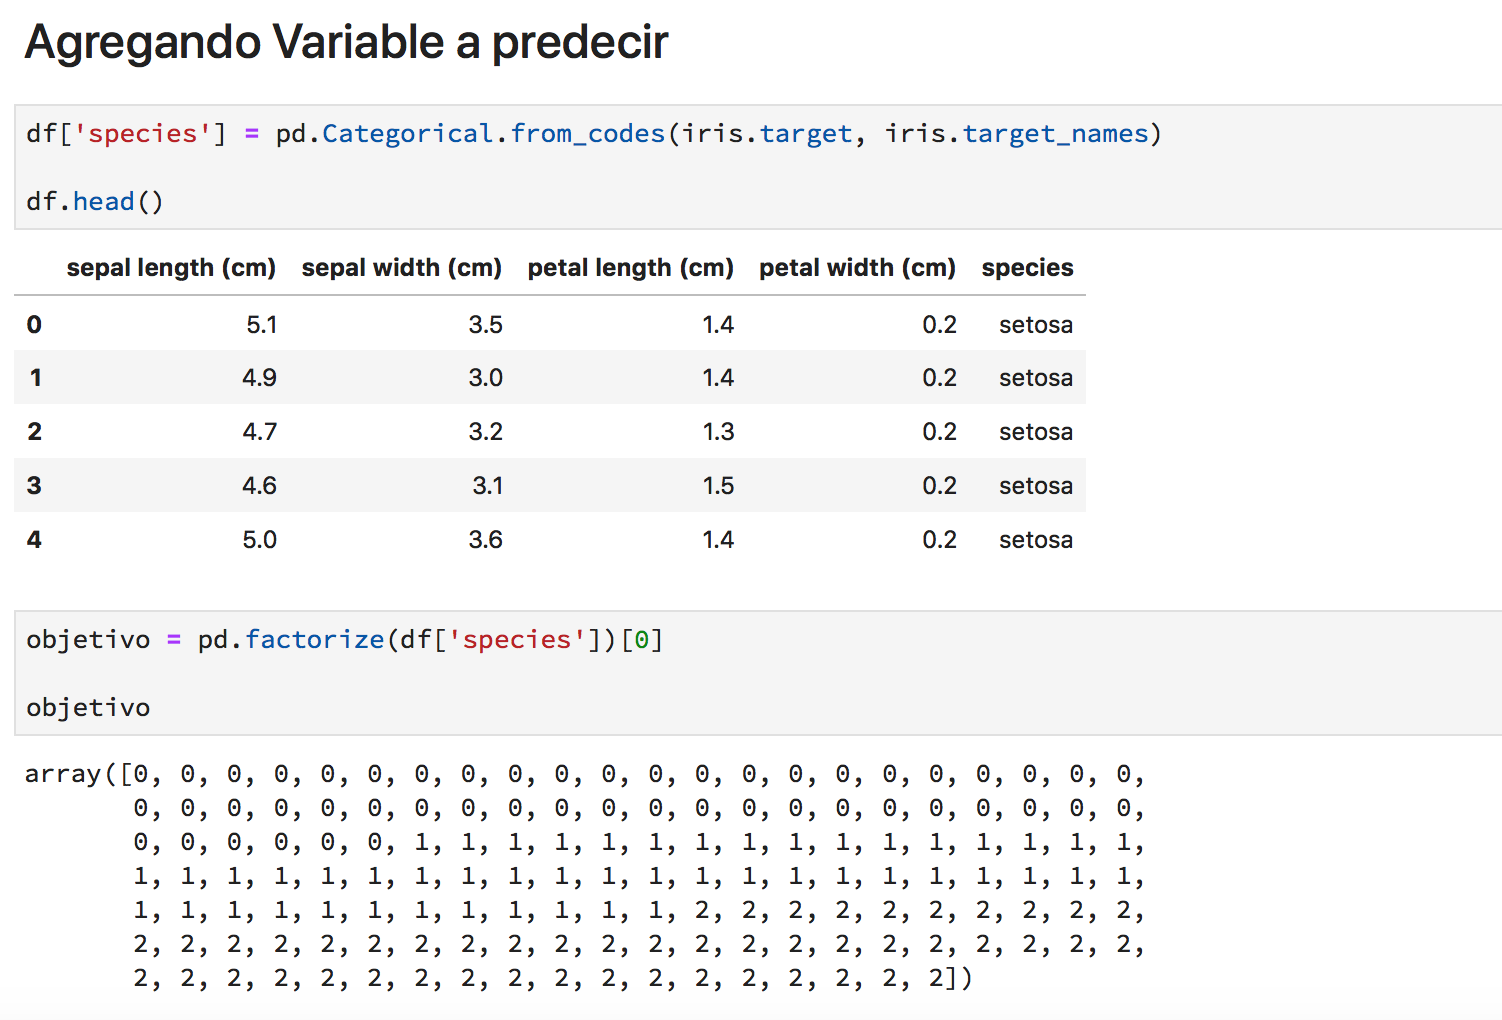
\includegraphics{images/bos2.png}
\caption{\label{fig:"R2"}}
\end{figure}

Para crear el modelo usamos la función \emph{RandomForestClasifier()} y \emph{.fit()} para entrenar el modelo.
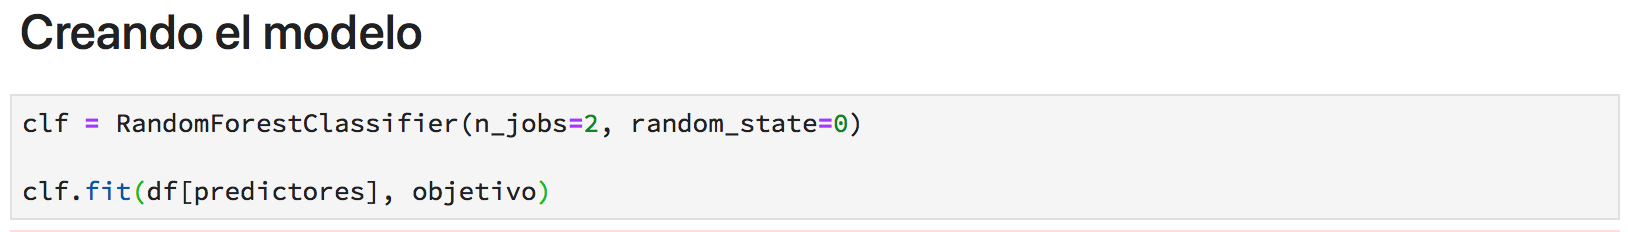
\includegraphics{images/bos3.png}

Finalmente, con \emph{.predict()} realizamos predicciones con nuestro modelo.

\begin{figure}
\centering
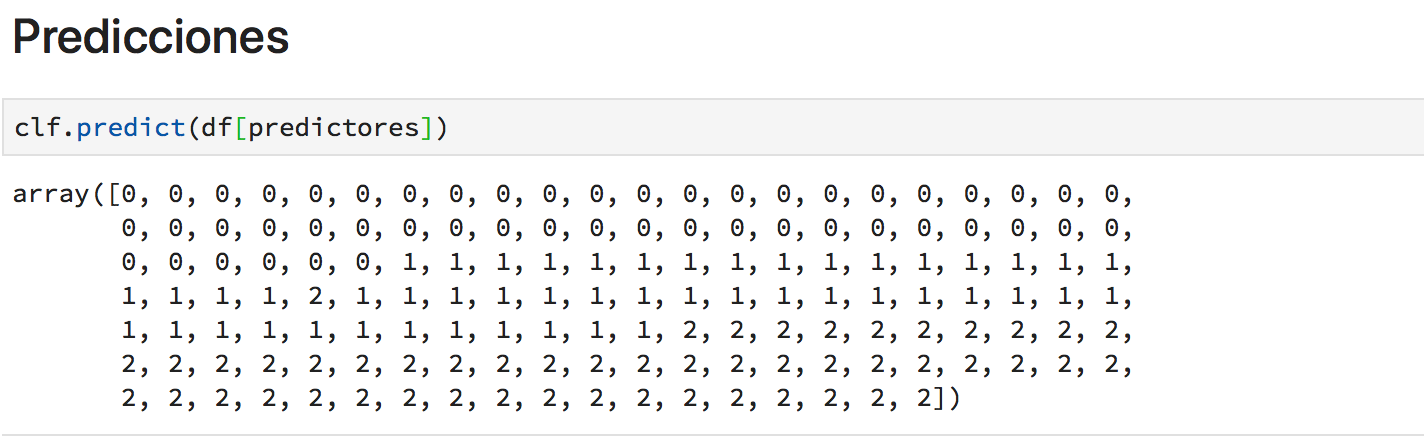
\includegraphics{images/bos4.png}
\caption{\label{fig:"R2"}}
\end{figure}

\cleardoublepage

\hypertarget{appendix-apendice}{%
\appendix \addcontentsline{toc}{chapter}{\appendixname}}


\hypertarget{herramientas-de-software}{%
\chapter{Herramientas de software}\label{herramientas-de-software}}

Para aquellos que no están familiarizados con los paquetes de software necesarios para usar R Markdown, damos una breve introducción sobre la instalación y mantenimiento de estos paquetes.

\hypertarget{r-y-paquetes-de-r}{%
\section{\texorpdfstring{\emph{R} y paquetes de \emph{R}}{R y paquetes de R}}\label{r-y-paquetes-de-r}}

\emph{R} puede descargarse e instalarse desde cualquier réplica de CRAN (Comprehensive R Archive Network), por ejemplo de \url{https://cran.rstudio.com} . Tenga en cuenta que existirán algunas nuevas versiones de \emph{R} cada año, y es posible que desee actualizar \emph{R} de vez en cuando.

Para instalar el paquete \emph{bookdown}, puede escribir en R:

\begin{Shaded}
\begin{Highlighting}[]
\KeywordTok{install.packages}\NormalTok{(}\StringTok{"bookdown"}\NormalTok{)}
\end{Highlighting}
\end{Shaded}

De esta manera se instalan todos los paquetes \emph{R} requeridos. También puede elegir instalar todos los paquetes opcionales, si no le importa demasiado si estos paquetes serán usados realmente para compilar su libro (como \textbf{htmlwidgets}):

\begin{Shaded}
\begin{Highlighting}[]
\KeywordTok{install.packages}\NormalTok{(}\StringTok{"bookdown"}\NormalTok{, }\DataTypeTok{dependencies =} \OtherTok{TRUE}\NormalTok{)}
\end{Highlighting}
\end{Shaded}

Si quiere probar la versión de desarrollo de \textbf{bookdown} en \emph{GitHub}, primero tiene que instalar \textbf{devtools}:

\begin{Shaded}
\begin{Highlighting}[]
\ControlFlowTok{if}\NormalTok{ (}\OperatorTok{!}\KeywordTok{requireNamespace}\NormalTok{(}\StringTok{'devtools'}\NormalTok{)) }\KeywordTok{install.packages}\NormalTok{(}\StringTok{'devtools'}\NormalTok{)}
\NormalTok{devtools}\OperatorTok{::}\KeywordTok{install_github}\NormalTok{(}\StringTok{'rstudio/bookdown'}\NormalTok{)}
\end{Highlighting}
\end{Shaded}

Los paquetes \emph{R} también se actualizan constantemente en \emph{CRAN} o \emph{GitHub}, por lo que es posible que desee actualizarlos de vez en cuando:

\begin{Shaded}
\begin{Highlighting}[]
\KeywordTok{update.packages}\NormalTok{(}\DataTypeTok{ask =} \OtherTok{FALSE}\NormalTok{)}
\end{Highlighting}
\end{Shaded}

Aunque no es necesario, el IDE de RStudio puede hacer muchas cosas mucho más fáciles cuando se trabaja en proyectos relacionados con R. El IDE de RStudio se puede descargar desde \url{https://www.rstudio.com}

\hypertarget{pandoc}{%
\section{Pandoc}\label{pandoc}}

Un documento R Markdown (\emph{.Rmd}) es primero compilado a Markdown (\emph{.md}) a través del paquete \emph{knitr}, y luego \emph{Markdown} es compilado a otros formatos de salida (como \emph{LaTeX} o \emph{HTML}) a través de \emph{Pandoc}. Este proceso está automatizado a través del paquete \emph{rmarkdown}. No es necesario instalar \emph{knitr} o \emph{rmarkdown} por separado, ya que son los paquetes requeridos de \emph{bookdown} y se instalarán automáticamente cuando instale \emph{bookdown}. Sin embargo, \emph{Pandoc} no es un paquete \emph{R}, por lo que no se instalará automáticamente cuando instale \emph{bookdown}. Puede seguir las instrucciones de instalación en la página principal de Pandoc (\url{http://pandoc.org}) para instalar \emph{Pandoc}, pero si utiliza el \emph{IDE} de \emph{RStudio}, no necesita instalar \emph{Pandoc} por separado, porque \emph{RStudio} incluye una copia de Pandoc. El número de versión de \emph{Pandoc} se puede obtener a través de:

\begin{Shaded}
\begin{Highlighting}[]
\NormalTok{rmarkdown}\OperatorTok{::}\KeywordTok{pandoc_version}\NormalTok{()}
\CommentTok{## [1] '2.3.1'}
\end{Highlighting}
\end{Shaded}

Si encuentra esta versión demasiado baja y hay características de \emph{Pandoc} sólo en una versión posterior, puede instalar la versión posterior de \emph{Pandoc}, y \emph{rmarkdown} llamará a la versión más reciente en lugar de su versión incorporada.

\hypertarget{latex}{%
\section{LaTeX}\label{latex}}

\emph{LaTeX} es necesario sólo si desea convertir su libro a \emph{PDF}. La elección típica de la distribución \emph{LaTeX} depende de su sistema operativo. Los usuarios de \emph{Windows} pueden considerar \emph{MiKTeX} (\url{http://miktex.org}), los usuarios de \emph{Mac OS X} pueden instalar \emph{MacTeX} (\url{http://www.tug.org/mactex/}), y los usuarios de \emph{Linux} pueden instalar \emph{TeXLive} (\url{http://www.tug.org/texlive}). Visite \url{https://www.latex-project.org/get/} para obtener más información sobre LaTeX y su instalación.

La mayoría de las distribuciones \emph{LaTeX} ofrecen un paquete mínimo/básico y un paquete completo. Puede instalar el paquete básico si tiene poco espacio de disco y sabe cómo instalar los paquetes \emph{LaTeX} más tarde. El paquete completo es a menudo significativamente más grande en tamaño, ya que contiene todos los paquetes de \emph{LaTeX}, y es poco probable que se encuentre con el problema de que le falten paquetes en \emph{LaTeX}.

Los mensajes de error de \emph{LaTeX} pueden ser oscuros para los principiantes, pero puede encontrar soluciones buscando el mensaje de error en línea (tiene buenas posibilidades de terminar en \emph{StackExchange}). De hecho, el código \emph{LaTeX} convertido a partir de \emph{R Markdown} debería ser lo suficientemente seguro y no debería tener problemas frecuentes con \emph{LaTeX} a menos que haya introducido contenido \emph{LaTeX} en bruto en sus documentos \emph{Rmd}. El problema más común de \emph{LaTeX} debería ser la falta de paquetes \emph{LaTeX}, y el error puede parecerse a esto:

\begin{Shaded}
\begin{Highlighting}[]
\NormalTok{! LaTeX Error: File `titling.sty' not found.}

\NormalTok{Type X to quit or <RETURN> to proceed,}
\NormalTok{or enter new name. (Default extension: sty)}

\NormalTok{Enter file name: }
\NormalTok{! Emergency stop.}
\NormalTok{<read *> }
         
\NormalTok{l.107 ^^M}

\NormalTok{pandoc: Error producing PDF}
\NormalTok{Error: pandoc document conversion failed with error 43}
\NormalTok{Execution halted}
\end{Highlighting}
\end{Shaded}

Esto significa que usó un paquete que contiene \emph{titling.sty}, pero no fue instalado. Los nombres de los paquetes \emph{LaTeX} suelen ser los mismos que los de los archivos \emph{.sty}, por lo que en este caso, puede intentar instalar el paquete de titulación. Tanto \emph{MiKTeX} como \emph{MacTeX} proporcionan una interfaz gráfica de usuario para gestionar paquetes. Puede encontrar el administrador de paquetes de \emph{MiKTeX} en el menú de inicio, y el administrador de paquetes de \emph{MacTeX} en la aplicación \emph{``TeX Live Utility''}. Escriba el nombre del paquete o el nombre del archivo para buscar el paquete e instalarlo. \emph{TeXLive} puede ser un poco más complicado: si usa los paquetes \emph{TeXLive} preconstruidos de su distribución de \emph{Linux}, necesita buscar en el repositorio de paquetes y sus palabras clave pueden coincidir con otros paquetes que no sean de \emph{LaTeX}. A veces resulta frustrante usar las colecciones de paquetes predefinidas en \emph{Linux}, y es mucho más fácil instalar \emph{TeXLive} desde el código fuente, en cuyo caso puede administrar paquetes usando el comando \emph{tlmgr}. Por ejemplo, puede buscar \emph{titling.sty} desde el repositorio de paquetes de \emph{TeXLive}:

\begin{Shaded}
\begin{Highlighting}[]
\ExtensionTok{tlmgr}\NormalTok{ search --global --file titling.sty}
\CommentTok{# titling:}
\CommentTok{#    texmf-dist/tex/latex/titling/titling.sty}
\end{Highlighting}
\end{Shaded}

Una vez que haya averiguado el nombre del paquete, puede instalarlo por medio de:

\begin{Shaded}
\begin{Highlighting}[]
\ExtensionTok{tlmgr}\NormalTok{ install titling  # may require sudo}
\end{Highlighting}
\end{Shaded}

Las distribuciones y paquetes de \emph{LaTeX} también se actualizan de vez en cuando, y puede considerar actualizarlos especialmente cuando tenga problemas con \emph{LaTeX}. Puede encontrar la versión de su distribución LaTeX por:

\begin{Shaded}
\begin{Highlighting}[]
\KeywordTok{system}\NormalTok{(}\StringTok{'pdflatex --version'}\NormalTok{)}
\CommentTok{## pdfTeX 3.14159265-2.6-1.40.19 (TeX Live 2018)}
\CommentTok{## kpathsea version 6.3.0}
\CommentTok{## Copyright 2018 Han The Thanh (pdfTeX) et al.}
\CommentTok{## There is NO warranty.  Redistribution of this software is}
\CommentTok{## covered by the terms of both the pdfTeX copyright and}
\CommentTok{## the Lesser GNU General Public License.}
\CommentTok{## For more information about these matters, see the file}
\CommentTok{## named COPYING and the pdfTeX source.}
\CommentTok{## Primary author of pdfTeX: Han The Thanh (pdfTeX) et al.}
\CommentTok{## Compiled with libpng 1.6.34; using libpng 1.6.34}
\CommentTok{## Compiled with zlib 1.2.11; using zlib 1.2.11}
\CommentTok{## Compiled with xpdf version 4.00}
\end{Highlighting}
\end{Shaded}

\bibliography{book.bib,packages.bib}

\backmatter
\printindex

\end{document}
